\documentclass[11pt,aspectratio=169,usenames,dvipsnames]{beamer}
%\beamerdefaultoverlayspecification{<+->}
\usefonttheme[onlymath]{serif}
%\usetheme{Madrid}
%\usetheme{metropolis}

\usetheme{Madrid}
\usetheme[subsectionpage=progressbar]{metropolis} 

\usepackage[utf8]{inputenc}
\usepackage{amsmath,bbding}
\usepackage{amsfonts}
\usepackage{amssymb}
\usepackage{subfig}
\usepackage{colortbl}
\usepackage{xcolor}
\definecolor{myorange}{HTML}{f07e26}
% \usepackage{tabularx}

%\author{\textbf{Mostafa Sadeghi}\\
%Perception team, INRIA Grenoble Rh\^one-Alpes, France\\}
%%\title{Deep Latent Variable Generative Models: Application to Audio-visual Speech Enhancement}
%
%\title{Unsupervised Audio-visual Speech Enhancement based on Variational Autoencoders}
%
%%\addtobeamertemplate{navigation symbols}{}{%
%%\usebeamerfont{footline}%
%%\usebeamercolor[fg]{footline}%
%%\hspace{1em}%
%%\insertframenumber/\inserttotalframenumber
%%}

% logos for the first frame
\titlegraphic{%
	%  \includegraphics[width=.2\textwidth]{example-image-a}\hfill
	%  \includegraphics[width=.2\textwidth]{example-image-b}\hfill
	\includegraphics[width=.2\textwidth]{logos/inriaLogo} \hfill \includegraphics[width=.12\textwidth]{logos/logo-uga.png} \hfill \includegraphics[width=.07\textwidth]{logos/logo-ljk.png} \hfill \includegraphics[scale=0.23]{logos/miaiLogo}  %\includegraphics[scale=0.13]{logo_gipsa-lab.png}
}

% first frame
\makeatletter

\setbeamertemplate{title page}{
	\begin{minipage}[b][\paperheight]{\textwidth}
		\centering
		\vfill%
		\ifx\inserttitle\@empty\else\usebeamertemplate*{title}\fi
		\ifx\insertsubtitle\@empty\else\usebeamertemplate*{subtitle}\fi
		\usebeamertemplate*{title separator}
		\ifx\beamer@shortauthor\@empty\else\usebeamertemplate*{author}\fi
		\ifx\insertinstitute\@empty\else\usebeamertemplate*{institute}\fi
		\vfill
		\ifx\inserttitlegraphic\@empty\else\inserttitlegraphic\fi
		\vspace*{0.25cm}
	\end{minipage}
}
\setbeamertemplate{title}{
	%  \raggedright%
	\linespread{1.0}%
	\inserttitle% 
	\par%
	\vspace*{0.5em}
}
\setbeamertemplate{subtitle}{
	%  \raggedright%
	\insertsubtitle%
	\par%
	\vspace*{0.5em}
}
\makeatother

\setbeamerfont{title}{size=\Large}
\setbeamerfont{author}{size=\small}
\setbeamerfont{institute}{size=\scriptsize}

\title{Probabilistic generative models for audio-visual processing}
\author{Xavier Alameda-Pineda}

\institute{
RobotLearn team, Inria at University Grenoble-Alpes,\\ Jean-Kuntzman CNRS Laboratory, Multidisciplinary Institute of Artificial Intelligence
}

\newcommand{\E}{\mathbb{E}}
\usepackage{multimedia}
\usepackage{animate}
\usepackage{hyperref}
\usepackage{tikz}
\usepackage{math}
\usepackage{makecell}
\usepackage{booktabs}
\usepackage{multirow}

%\setbeamertemplate{navigation symbols}{}
%\setbeamertemplate{footline}[page number]{}s
\makeatletter
\let\save@measuring@true\measuring@true
\def\measuring@true{%
  \save@measuring@true
  \def\beamer@sortzero##1{\beamer@ifnextcharospec{\beamer@sortzeroread{##1}}{}}%
  \def\beamer@sortzeroread##1<##2>{}%
  \def\beamer@finalnospec{}%
}
\makeatother
\newcommand{\bs}{\boldsymbol}
\date{March 19, 2020}
%\DeclareMathOperator*{\argmax}{arg\max}

\usepackage[many]{tcolorbox}   

\newtcolorbox{mybox2}[1]{%
	tikznode boxed title,
	enhanced,
	arc=3mm,
	interior style={white},
	attach boxed title to top center= {yshift=-\tcboxedtitleheight/2},
	%    fonttitle=\bfseries,
	colbacktitle=white,
	coltitle=black,
	boxed title style={size=normal,colframe=white,boxrule=0pt}, 
	left=1mm, 
	right=1mm, 
	top=3mm, 
	bottom=2mm, 
	nobeforeafter,
	boxrule=.2mm,
	title={#1}
}

\newcommand\blfootnote[1]{%
	\begingroup
	\renewcommand\thefootnote{}\footnote{\scriptsize #1}%
	\addtocounter{footnote}{-1}%
	\endgroup
}

\setbeamertemplate{footline}{
	\usebeamercolor[fg]{page number in head}%
	\usebeamerfont{page number in head}%
	\begin{flushright}
	\insertframenumber$\quad$
	\end{flushright}\vspace{-2mm}
}

\newcommand{\argmax}{\operatornamewithlimits{argmax}}
\newcommand{\argmin}{\operatornamewithlimits{argmin}}

% \usepackage{tikz}
\usepackage{xstring}

\usetikzlibrary{bayesnet,calc}
\usetikzlibrary{shapes.geometric}
\tikzset{  net/.style={draw,trapezium,trapezium angle=75,shape border rotate=270} }
\tikzset{  rnn/.style={draw,rectangle} }
\usetikzlibrary{fit,positioning}
\newcommand{\drawNodes}[2]{}
\newcommand{\denselyConnectNodes}[2]{}

\newcommand{\mylz}{{\color{red}z}}
\newcommand{\myox}{{\color{green}x}}
\newcommand{\myls}{{\color{red}s}}
\newcommand{\myos}{{\color{green}s}}
\newcommand{\myov}{{\color{green}v}}

\usepackage{neuralnetwork}


\begin{document}

%%%%%%%%%%%%%%%%%%%%%%%%%%%%%%%%%%%%%%%%%%%%%%%%%%%%%%%%%%%%%%%%%%%%%%%%%%%%
\begin{frame}[noframenumbering,plain]
\titlepage
\end{frame}



%%%%%%%%%%%%%%%%%%%%%%%%%%%%%%%%%%%%%%%%%%%%%%%%%%%%%%%%%%%%%%%%%%%%%%%%%%%%
\begin{frame}{Why unsupervised learning?}
Imagine a system for \{person tracking, speech denoising, body pose estimation, ...\} in: 
\begin{figure}
 \includegraphics[width=0.3\textwidth]{images/26WAITING-jumbo.jpg}
 \hspace{2mm}
 \includegraphics[width=0.3\textwidth]{images/socialgathering.jpg}
 \hspace{2mm}
 \includegraphics[width=0.3\textwidth]{images/waitingroom.jpg}\vspace{-8mm}
\end{figure}
{\tiny [Images under Creative Commons license]}

We would like to avoid re-annotating for every new environment $\rightarrow$ Interest in unsupervised learning (and/or unsupervised domain adaptation).
\end{frame}

%%%%%%%%%%%%%%%%%%%%%%%%%%%%%%%%%%%%%%%%%%%%%%%%%%%%%%%%%%%%%%%%%%%%%%%%%%%%
\begin{frame}{And probabilistic learning?}
 Probabilistic generative models aim to learn a (parametric) \emph{distribution} $p_{\bs{\theta}}(\bs{x})$ that approximates the complex data distribution $ p_{\text{\tiny{data}}}(\bs{x})$:
\begin{figure}
\centering
    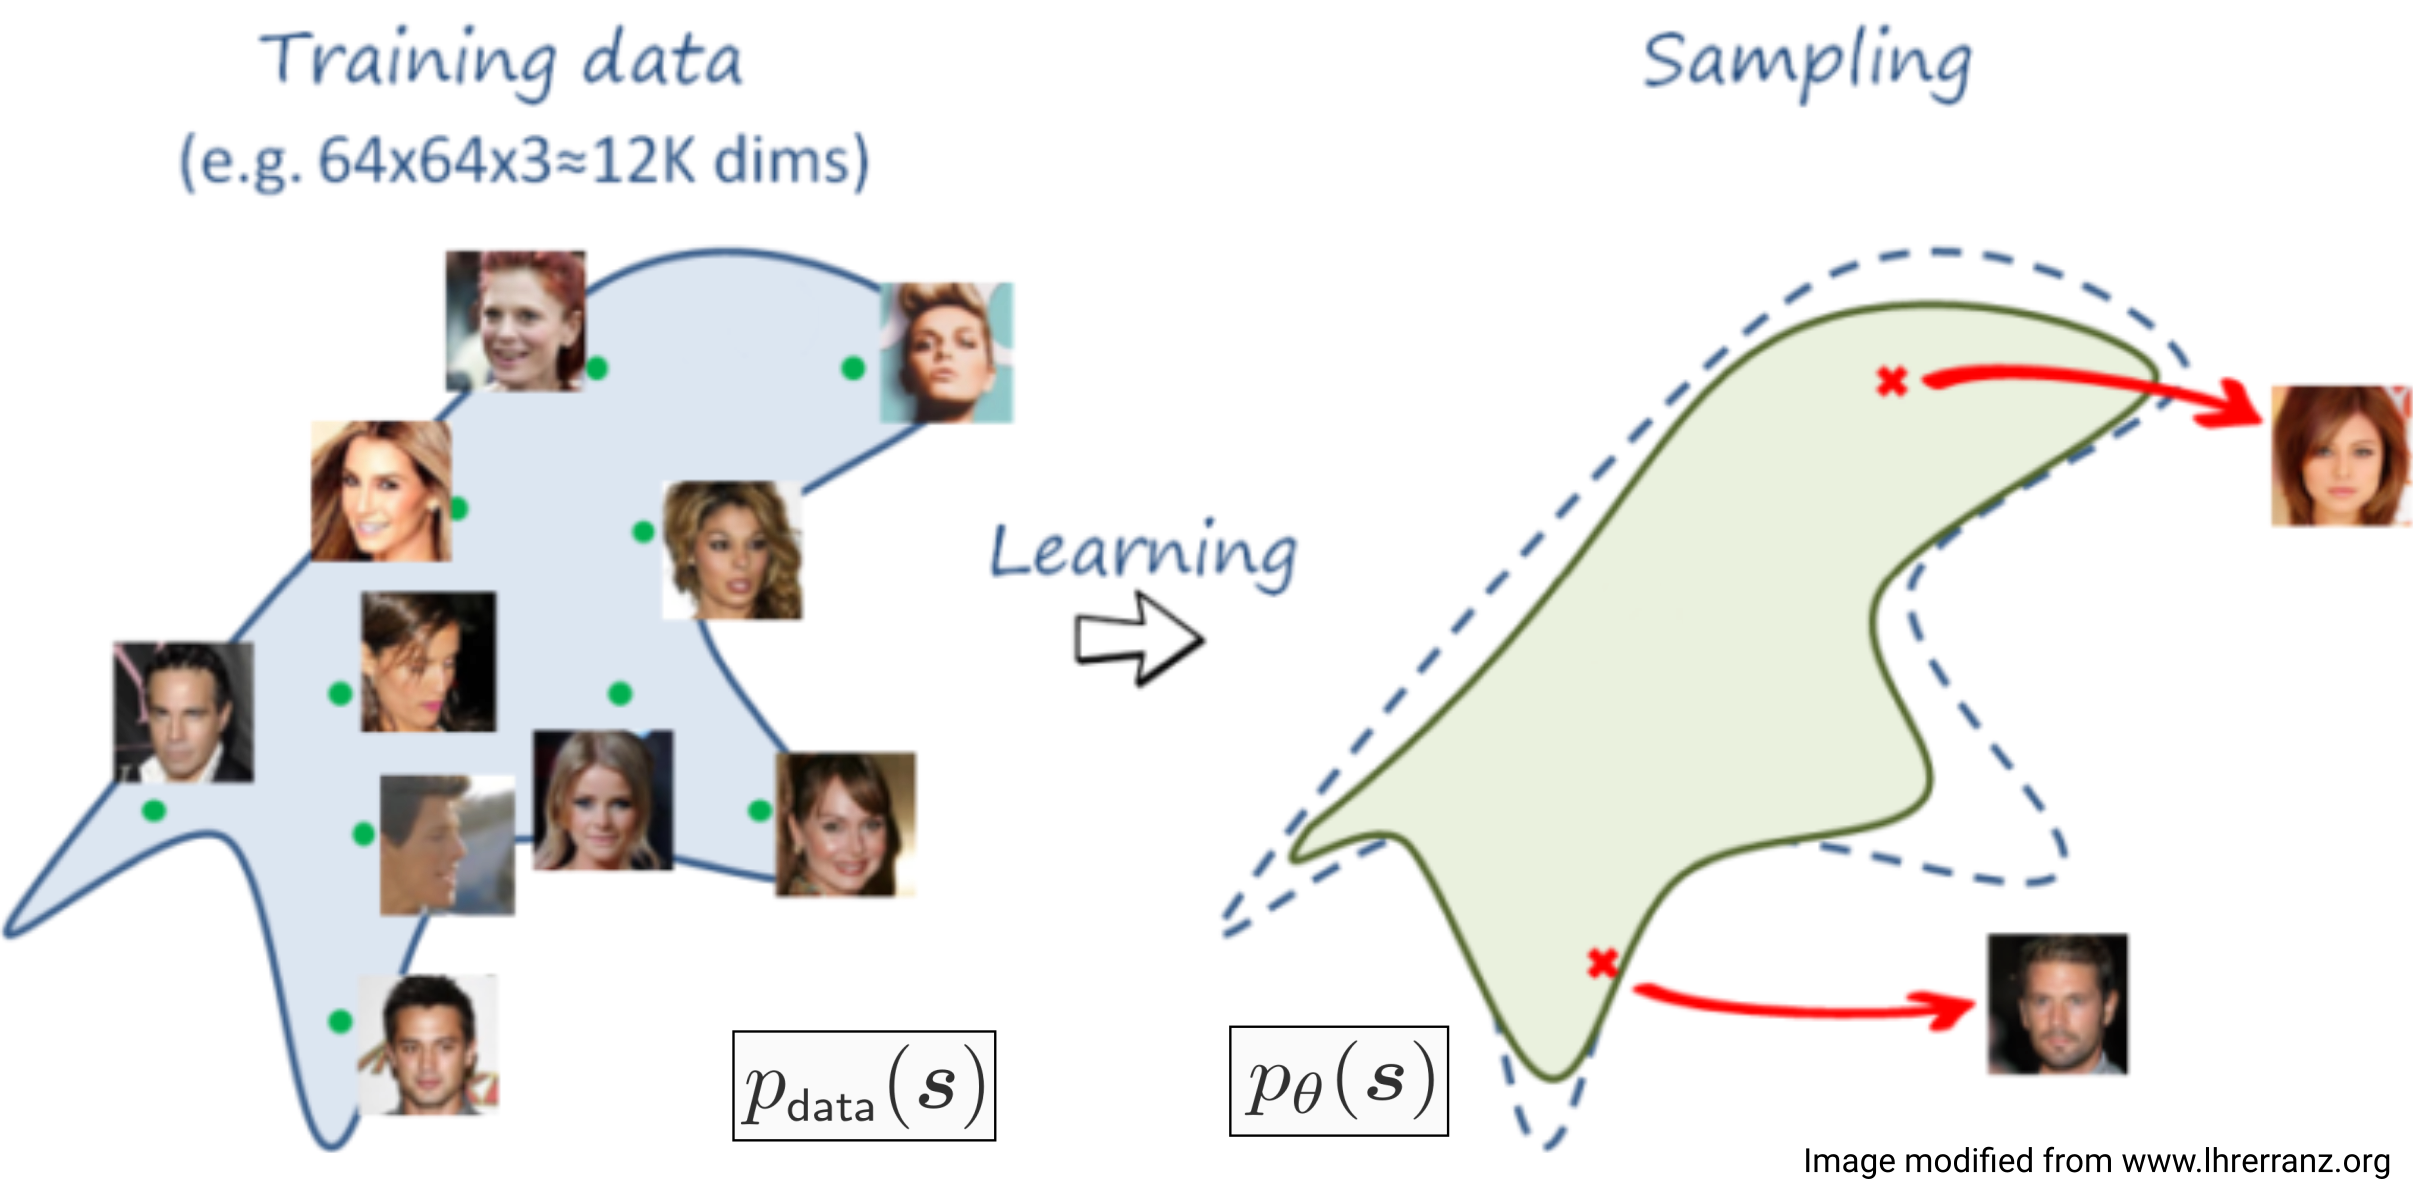
\includegraphics[scale=0.45]{images/generative-model-mod.png}
\end{figure}

% Probabilistic models are interesting because:
\begin{itemize}
 \item Once learned, we can (ideally) sample new data.
 \item We can jointly learn them with other probabilistic models using \textit{maximum likelihood}.
\end{itemize}
\end{frame}

%%%%%%%%%%%%%%%%%%%%%%%%%%%%%%%%%%%%%%%%%%%%%%%%%%%%%%%%%%%%%%%%%%%%%%%%%%%%
\begin{frame}{The Kullback-Leibler divergence and the ML formulation}
The Kullback-Leilbler (KL) divergence between two distributions writes:
\begin{equation*}
 {\color{myorange} \underbrace{D_{\text{KL}}(p(\bs{x})\|q(\bs{x})) = -\E_{p(\bs{x})}\left[\log\frac{q(\bs{x})}{p(\bs{x})}\right]}_{\text{Need your help!}} } = -\int_{\cal X} p(\bs{x})\log\frac{q(\bs{x})}{p(\bs{x})}\textrm{d}\bs{x} \left\{\begin{array}{l} \geq 0 \\ \neq D_{\text{KL}}(q(\bs{x})\|p(\bs{x})) \end{array}\right.
\end{equation*}
$D_{\text{KL}}(p(\bs{x})\|q(\bs{x})) = 0 \Leftrightarrow p(\bs{x})=q(\bs{x})$.\vspace{10mm}\\

\pause
Given a training set $\{\bs{x}_i\}_{i=1}^N, \bs{x}_i\sim p_{\text{\tiny{data}}}(\bs{x})$, ML minimizes the KL divergence:
\begin{align*}
\bs{\theta}^*=&\argmin_{\bs{\theta}}~ D_{\text{KL}}\Big(p_{\text{\tiny{data}}}(\bs{x}) \parallel p_{\bs{\theta}}(\bs{x})\Big)=\argmin_{\bs{\theta}}~-\E_{p_{\text{\tiny{data}}}}\Big[ \log \frac{p_{\bs{\theta}}(\bs{x})}{p_{\text{\tiny{data}}}(\bs{x})}\Big]\\
=& \argmax_{\bs{\theta}}~\E_{p_{\text{\tiny{data}}}}\Big[ \log {p_{\bs{\theta}}(\bs{x})}\Big]
\approx \boxed{\argmax_{\bs{\theta}}~{\frac{1}{N}\sum_{i=1}^N \log {p_{\bs{\theta}}(\bs{x}_i)}}}
\end{align*}
\end{frame}

%%%%%%%%%%%%%%%%%%%%%%%%%%%%%%%%%%%%%%%%%%%%%%%%%%%%%%%%%%%%%%%%%%%%%%%%%%%%
\begin{frame}{Interest of Latent Variables}
\begin{itemize}
 \item Speech enhancement: noisy speech (observation), clean speech (latent variable)
%  $\rightarrow$ Get rid of noise heard together with speech.
 \item Person tracking: detections (observation), person positions (latent variable)
%  $\rightarrow$ Track occluded persons, filter over time.
 \item Representation learning: raw data (observation), representation (latent variable)
%  $\rightarrow$ Compute an optimal compact representation of the raw data.
\end{itemize}\pause

Let $\bs{z}$ denote the latent variable:
\[
\begin{cases}
\bs{z}\sim p_{\bs{\theta}}(\bs{z})\\
\bs{x}|\bs{z}\sim p_{\bs{\theta}}(\bs{x}|\bs{z})
\end{cases}\rightarrow~ {\color{myorange}p_{\bs{\theta}}(\bs{x})=\int p_{\bs{\theta}}(\bs{x}, \bs{z}) \textrm{d}\bs{z}} = \int p_{\bs{\theta}}(\bs{x}|\bs{z})p_{\bs{\theta}}(\bs{z}) \textrm{d}\bs{z}\]

\pause
\textbf{New samples:} Draw $ \hat{\bs{z}} \sim p_{\bs{\theta}}(\bs{z}) $, then draw a new sample $ \hat{\bs{x}} \sim p_{\bs{\theta}}(\bs{x}|\hat{\bs{z}}) $.

\textbf{Learning:} How to estimate $\bs{\theta}$ with the ML formulation?

\textbf{Inference:} How to get the most likely latent $p_{\bs{\theta}}(\bs{z}
|\bs{x})$?
\end{frame}

%
% %%%%%%%%%%%%%%%%%%%%%%%%%%%%%%%%%%%%%%%%%%%%%%%%%%%%%%%%%%%%%%%%%%%%%%%%%%%%
% \begin{frame}{Lecture Organisation}
% \begin{itemize}
%  \item Lecture 1: Probabilistic learning with latent variables, GMM and the exact EM algorithm, probabilistic PCA and VAE.
%  \item Lecture 2: The variational EM algoritm, mixtures of VAEs, application to audio-visual speech enhancement.
%  \item Lecture 3: Dynamical variational autoencoders, application to speech enhancement.
% \end{itemize}
%
% Connections to other lectures:
% \begin{itemize}
%  \item Matthias Bauer: from PPCA/VAE to diffusion models.
%  \item Steve Kroon: normalising flows and their use with VAEs.
% \end{itemize}
%
%  \alert{I am fully available for discussing/chatting with y'all!}
% \end{frame}
%
% %%%%%%%%%%%%%%%%%%%%%%%%%%%%%%%%%%%%%%%%%%%%%%%%%%%%%%%%%%%%%%%%%%%%%%%%%%%%
% \begin{frame}{Disclaimer}
%  We will be discussing the fundamentals of probabilistic learning, and a series of advanced models and combinations.\vspace{3mm}\\
%
%  There will be (at least in my courses) a non-negligeable amount of equations:
%  \begin{itemize}
%   \item The \textit{details} of these equations are not important.
%   \item The general principle on how to get them and their interpretation are.
%   \item These should help you (i) interpret the resuts of existing models and (ii) derive your own models.
%  \end{itemize}
%
% \end{frame}

% %%%%%%%%%%%%%%%%%%%%%%%%%%%%%%%%%%%%%%%%%%%%%%%%%%%%%%%%%%%%%%%%%%%%%%%%%%%%
% \begin{frame}[noframenumbering]{Lecture's Outline}
% \textcolor{red}{\Huge TODO}%\tableofcontents
% \end{frame}


%%%%%%%%%%%%%%%%%%%%%%%%%%%%%%%%%%%%%%%%%%%%%%%%%%%%%%%%%%%%%%%%%%%%%%%%%%%%
%%%%%%%%%%%%%%%%%%%%%%%%%%%%%%%%%%%%%%%%%%%%%%%%%%%%%%%%%%%%%%%%%%%%%%%%%%%%
% \section{}
{\setbeamercolor{background canvas}{bg=mDarkTeal}
\setbeamercolor{background canvas}{fg=white}
\begin{frame}
 \centering
 \color{white}\large\bf From shallow GMMs to deep VAEs
\end{frame}}


\begin{frame}{Simple example: clustering}
    Definition: find groups of data points without labels.
    \begin{figure}
     \centering
     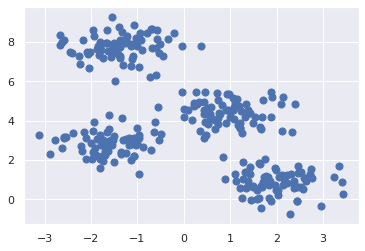
\includegraphics[width=0.45\textwidth]{images/clustering}
     \hspace{5mm}
     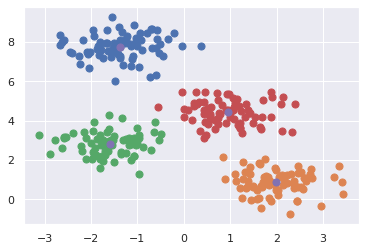
\includegraphics[width=0.45\textwidth]{images/clustering_done}
    \end{figure}
\end{frame}

% %%%%%%%%%%%%%%%%%%%%%%%%%%%%%%%%%%%%%%%%%%%%%%%%%%%%%%%%%%%%%%%%%%%%%%%%%%%%
% \begin{frame}{Very intuitive algorithm}
%     Very simple algorithm (called the $K$-means algorithm):
% %     \begin{columns}
% %      \begin{column}{0.55\textwidth}
%         \begin{enumerate}
%         \item Initialise randomly $K$ centroids.
%         \item Assign each data point to the closes centroid.
%         \item Recompute centroids from the assignments.
%         \item Iterate the past two steps.
%         \end{enumerate}
% %      \end{column}
% %      \begin{column}{0.45\textwidth}
% % %         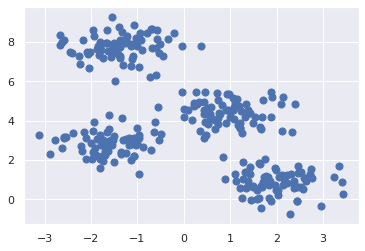
\includegraphics[width=1\textwidth]{images/clustering}
% % %         \movie[showcontrols]{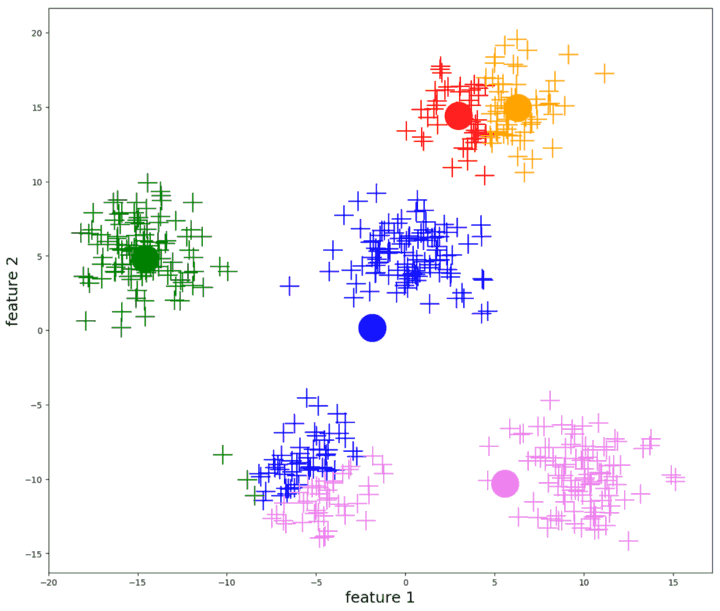
\includegraphics[width=\textwidth]{images/kmeans-clustering.png}}{images/kmeans-clustering.gif}
% %           \animategraphics[loop,autoplay,width=\textwidth]{1}{images/kmeans-clustering-}{0}{5}
% %      \end{column}
% %
% %     \end{columns}
%     \begin{figure}
%       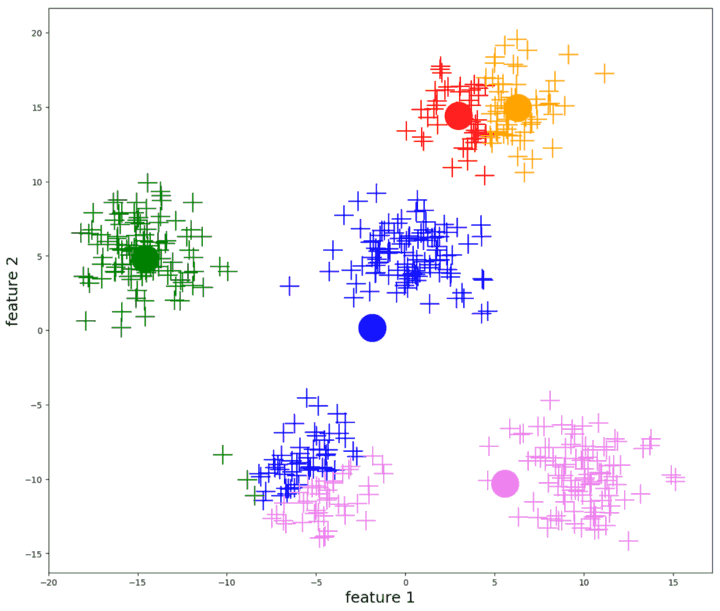
\includegraphics[width=0.2\textwidth]{images/kmeans-clustering-0}%
%       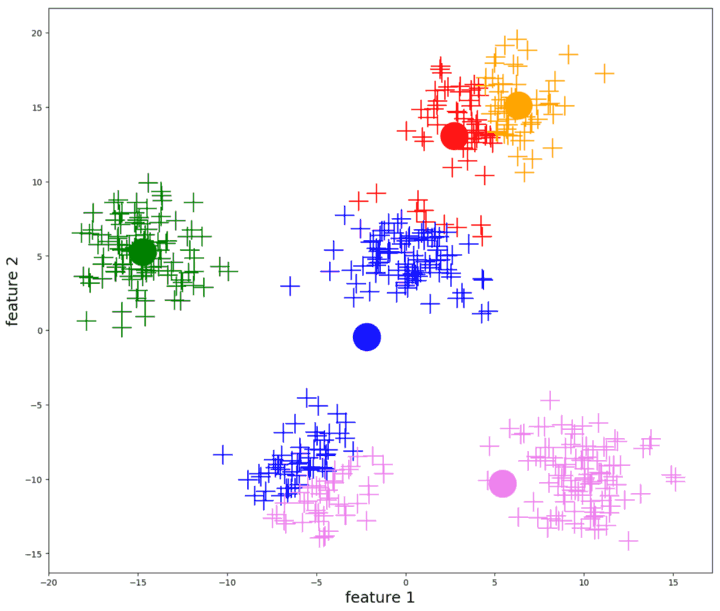
\includegraphics[width=0.2\textwidth]{images/kmeans-clustering-1}%
%       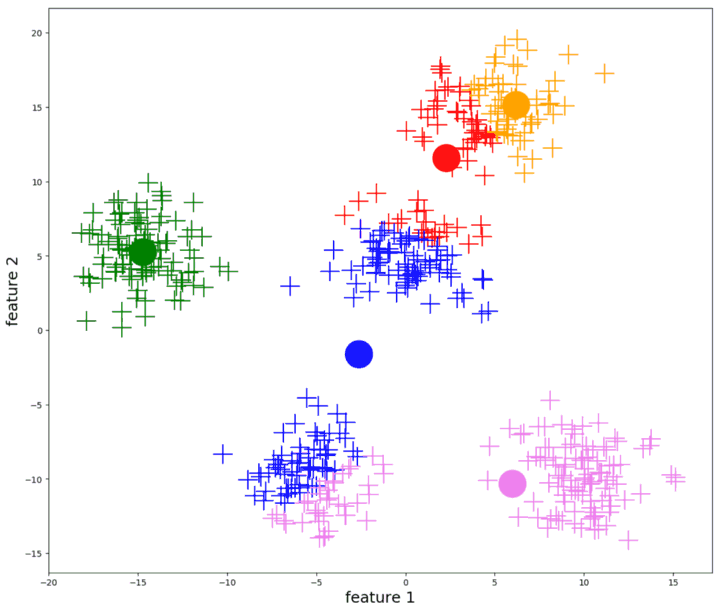
\includegraphics[width=0.2\textwidth]{images/kmeans-clustering-2}%
%       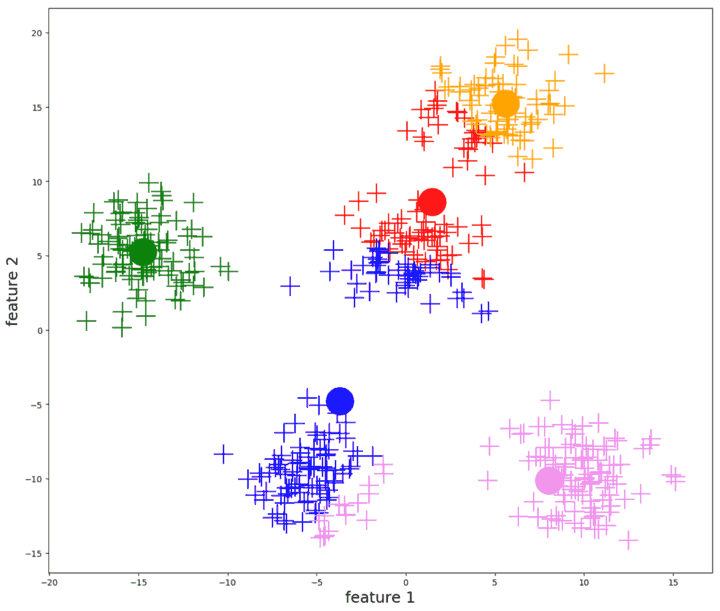
\includegraphics[width=0.2\textwidth]{images/kmeans-clustering-3}%
%       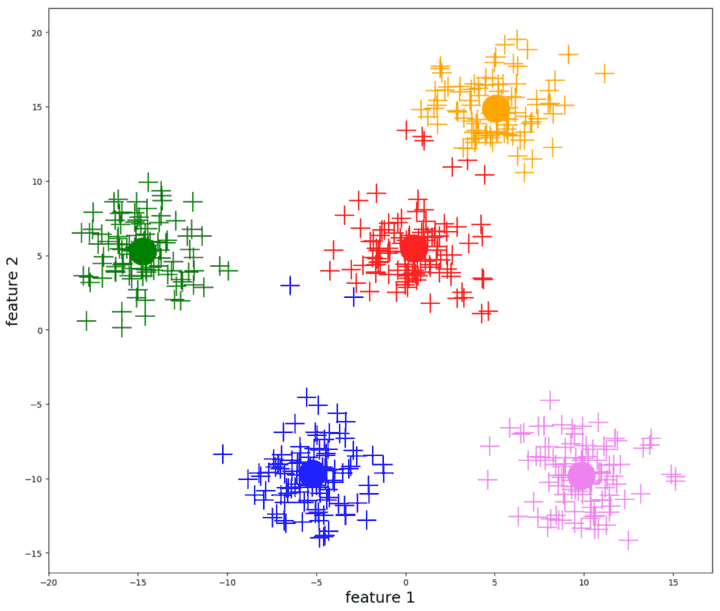
\includegraphics[width=0.2\textwidth]{images/kmeans-clustering-4}\vspace{-8mm}
%     \end{figure}
%     {\tiny [Images from \url{https://ai.plainenglish.io/}]}
%
%
% \end{frame}
%
% %%%%%%%%%%%%%%%%%%%%%%%%%%%%%%%%%%%%%%%%%%%%%%%%%%%%%%%%%%%%%%%%%%%%%%%%%%%%
% \begin{frame}{Important points of $K$-means}
%  The point-to-cluster assignment variable is unknown (latent, $\bs{z}$), and must be infered with the centroids (parameters of the model).
%
%
% %  \begin{block}{}
%   The assignment criterion is the Euclidean distance $\Rightarrow$ groups are spherical and equally populated a priori.
% %  \end{block}
%
%  \begin{figure}
%   \centering
%        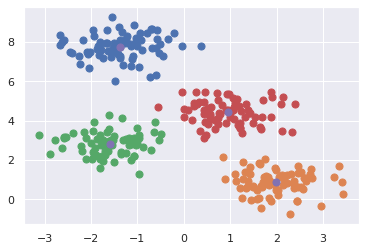
\includegraphics[width=0.45\textwidth]{images/clustering_done}
%      \hspace{5mm}
%      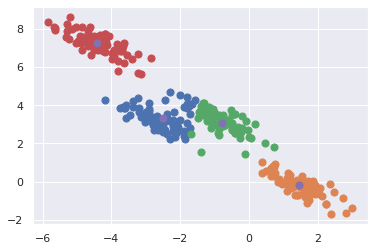
\includegraphics[width=0.45\textwidth]{images/clustering_fail}
%  \end{figure}
% \end{frame}


%%%%%%%%%%%%%%%%%%%%%%%%%%%%%%%%%%%%%%%%%%%%%%%%%%%%%%%%%%%%%%%%%%%%%%%%%%%%
\begin{frame}{The Gaussian Mixture Model (GMM)}
Definition:
\begin{itemize}
 \item For each $\bs{x}_n$ there is a latent variable $\bs{z}_n$ taking values from 1 to $K$: $\bs{z}_n\in\{1,\ldots,K\}$.\pause
 \item Its prior probability is defined as: $p(\bs{z}_n=k)=\pi_k\geq0$, with $\sum_{k=1}^K \pi_k = 1$.\pause
 \item Given $z_n$, the data point is modeled as a multivariate Gaussian:\vspace{-2mm}
 \[p(\bs{x}_n|\bs{z}_n=k) = \mathcal{N}(\bs{x}_n;\bs{\mu}_k,\bs{\Sigma}_k) \]
\end{itemize}
% \vspace{3mm}
Advantages:
 \begin{enumerate}
  \item Having $\pi_1,\ldots,\pi_K$ means that groups can be differently populated.
  \item The shape of the groups is modeled by $\bs{\Sigma}_k$.
  \item The parameters are: {\color{orange}$\bs{\theta}=\{\pi_k,\bs{\mu}_k,\bs{\Sigma}_k\}_{k=1}^K$}.
 \end{enumerate}
\end{frame}

%%%%%%%%%%%%%%%%%%%%%%%%%%%%%%%%%%%%%%%%%%%%%%%%%%%%%%%%%%%%%%%%%%%%%%%%%%%%
\begin{frame}{Maximum likelihood for GMM}
 Let's compute $p(\bs{x}_n)$
 \[ p(\bs{x}_n) = \sum_{k=1}^K p(\bs{x}_n,\bs{z}_n=k) = \sum_{k=1}^K \pi_k\mathcal{N}(\bs{x}_n;\bs{\mu}_k,\bs{\Sigma}_k).\]
 The log-likelihood:
 \[\mathcal{L}(\bs{\theta}|\bs{X}) = \sum_{n=1}^N \log  \sum_{k=1}^K \pi_k\mathcal{N}(\bs{x}_n;\bs{\mu}_k,\bs{\Sigma}_k),\]
 
 Computing directly ML by $\displaystyle\frac{\partial\mathcal{L}}{\partial\pi_k}=0$, $\displaystyle\frac{\partial\mathcal{L}}{\partial\bs{\mu}_k}=0$ or $\displaystyle\frac{\partial\mathcal{L}}{\partial\bs{\Sigma}_k}=0$ is very difficult.
\end{frame}

%%%%%%%%%%%%%%%%%%%%%%%%%%%%%%%%%%%%%%%%%%%%%%%%%%%%%%%%%%%%%%%%%%%%%%%%%%%%
%%%%%%%%%%%%%%%%%%%%%%%%%%%%%%%%%%%%%%%%%%%%%%%%%%%%%%%%%%%%%%%%%%%%%%%%%%%%
% \section{EM for GMM and beyond}

%%%%%%%%%%%%%%%%%%%%%%%%%%%%%%%%%%%%%%%%%%%%%%%%%%%%%%%%%%%%%%%%%%%%%%%%%%%%
\begin{frame}{(Expected complete-data) log-likelihood}
 We have seen that $\log p(\bs{x})$ does not work well with derivatives. However, $\log p(\bs{x},\bs{z})$ does!\vspace{3mm}\\
 
 \textbf{Problem}: $\bs{z}$ is not observed, thus $\sum_n\log p(\bs{x}_n,\bs{z}_n)$ is a random variable.\vspace{6mm}\\
 \pause

 Given an initial value of the parameters, $\bs{\theta}^0$, let's take the expectation w.r.t.\ the posterior distribution $p(\bs{z}|\bs{x},\bs{\theta}^0)$ {\footnotesize [we will justify this choice later on]}:
 \[\color{myorange}\mathcal{Q}(\bs{\theta},\bs{\theta}^0) = \sum_n \mathbb{E}_{p(\bs{z}_n|\bs{x}_n;\bs{\theta}^0)} \log p(\bs{x}_n,\bs{z}_n;\bs{\theta})\]
 
 This function is called: \textit{expected complete-data log-likelihood}, and is the main mathematical object when working with EM algorithms.
\end{frame}

%%%%%%%%%%%%%%%%%%%%%%%%%%%%%%%%%%%%%%%%%%%%%%%%%%%%%%%%%%%%%%%%%%%%%%%%%%%%
\begin{frame}{The EM algorithm for GMM}
 Given $\bs{\theta}^0$, we use the \textit{expected complete-data log-likelihood} $\mathcal{Q}$. For iteration $r=1,\ldots,R$:\vspace{2mm}
 \begin{enumerate}
  \item Expectation [E-step]:
  \[ \mathcal{Q}(\bs{\theta},\bs{\theta}^{r-1}) = \mathbb{E}_{p(\bs{z}|\bs{x};\bs{\theta}^{r-1})} \log p(\bs{x},\bs{z};\bs{\theta})\]\vspace{-5mm}
  \item Maximisation [M-step]: 
  \[ \bs{\theta}^r = \arg\max_{\bs{\theta}} \mathcal{Q}(\bs{\theta},\bs{\theta}^{r-1})\]
 \end{enumerate}
 {\footnotesize (observations $\bs{x}=\{\bs{x}_n\}_{n=1}^N$, latent variables $\bs{z}=\{\bs{z}_n\}_{n=1}^N$, parameters $\bs{\theta}=\{\pi_k,\bs{\mu}_k,\bs{\Sigma}_k\}_{k=1}^K$)}%\pause\vspace{4mm}
 
%   We can look back to $K$-means:
%  \begin{enumerate}
%   \item Infer latent variables (assignment) given the parameters (centroids) [E-step].
%   \item Estimate the parameters (centroids) given the assignments [M-step].
%  \end{enumerate}
\end{frame}

%%%%%%%%%%%%%%%%%%%%%%%%%%%%%%%%%%%%%%%%%%%%%%%%%%%%%%%%%%%%%%%%%%%%%%%%%%%%
\begin{frame}{The EM algorithm for GMM (II)}
\textbf{E-step} The posterior distribution writes:
\begin{equation*}
 p(\bs{z}_n=k|\bs{x}_n;\bs{\theta}^0) = \frac{p(\bs{z}_n=k;\bs{\theta}^0)p(\bs{x}_n|\bs{z}_n=k;\bs{\theta}^0)}{\sum_\ell p(\bs{z}_n=\ell;\bs{\theta}^0)p(\bs{x}_n|\bs{z}_n=\ell;\bs{\theta}^0)} =  \frac{\pi_k^0\mathcal{N}(\bs{x}_n;\bs{\mu}_k^0,\bs{\Sigma}_k^0)}{\sum_{\ell}\pi_\ell^0\mathcal{N}(\bs{x}_n;\bs{\mu}_\ell^0,\bs{\Sigma}_\ell^0)} = \eta_{nk}
\end{equation*}\pause

The expected complete-data log-likelihood writes:
\begin{equation*}
 \mathcal{Q}(\bs{\theta},\bs{\theta}^0) = \sum_{n=1}^N\sum_{k=1}^K \eta_{nk} \log \pi_k\mathcal{N}(\bs{x}_n;\bs{\mu}_k,\bs{\Sigma}_k)
\end{equation*}\pause

\textbf{M-step} The optimal value for $\bs{\mu}_k$ writes:
  \[\bs{\mu}_k^*=\frac{1}{\sum_{n=1}^N \eta_{nk}}\sum_{n=1}^N\eta_{nk}\bs{x}_n\]
\end{frame}

%%%%%%%%%%%%%%%%%%%%%%%%%%%%%%%%%%%%%%%%%%%%%%%%%%%%%%%%%%%%%%%%%%%%%%%%%%%%
\begin{frame}{But why does the EM work?}
 The main mathematical object in EM is $\mathcal{Q}$ {\footnotesize (The expected complete-data log-likelihood)}.\vspace{4mm}\\
 
 What is the relationship with the log-likelihood? Let's take any distribution of $\bs{z}$, $q(\bs{z})$:
%  \begin{align*}
% \log p(\bs{x})&= \mathbb{E}_{q(\bs{z})}\Big[\log p(\bs{x})\Big]\\
% &= \mathbb{E}_{q(\bs{z})}\Big[\log p(\bs{x})\frac{p(\bs{z}|\bs{x})q(\bs{z})}{p(\bs{z}|\bs{x})q(\bs{z})}\Big]\\
% &= \underbrace{\mathbb{E}_{q(\bs{z})}\Big[\log \frac{p(\bs{x})p(\bs{z}|\bs{x})}{q(\bs{z})}\Big]}_{\text{M-step - }\mathcal{Q}} +  \underbrace{D_{\text{KL}}\Big(q(\bs{z})\Big\lVert p(\bs{z}|\bs{x})\Big)}_{\text{E-step - KL}}
% \end{align*}
\begin{equation*}
\color{myorange} \log p(\bs{x}) = \underbrace{\mathbb{E}_{q(\bs{z})}\Big[\log \frac{p(\bs{x})p(\bs{z}|\bs{x})}{q(\bs{z})}\Big]}_{\text{M-step - }\mathcal{Q}} +  \underbrace{D_{\text{KL}}\Big(q(\bs{z})\Big\lVert p(\bs{z}|\bs{x})\Big)}_{\text{E-step - KL}}
\end{equation*}\pause
%
% \end{frame}
%
% %%%%%%%%%%%%%%%%%%%%%%%%%%%%%%%%%%%%%%%%%%%%%%%%%%%%%%%%%%%%%%%%%%%%%%%%%%%%
% \begin{frame}{But why does the EM work? (II)}
%  \begin{align*}
% \log p(\bs{x};\bs{\theta}) &= \underbrace{\mathbb{E}_{q(\bs{z})}\Big[\log \frac{p(\bs{x})p(\bs{z}|\bs{x})}{q(\bs{z})}\Big]}_{\text{M-step - }\mathcal{Q}} +  \underbrace{D_{\text{KL}}\Big(q(\bs{z})\Big\lVert p(\bs{z}|\bs{x})\Big)}_{\text{E-step - KL}}
% \end{align*}
Another interpretation. Given $\bs{\theta}^0$:
\begin{enumerate}
 \item Set $q(\bs{z})=p(\bs{z}|\bs{x};\bs{\theta}^0)$, minimise KL (thus maximize $\mathcal{Q}$) w.r.t.\ $q(\bs{z})$. The E-step reduces the distance between log-likelihood and $\mathcal{Q}$.
 \item Maximize $\mathcal{Q}$ w.r.t.\ $\bs{\theta}$:\vspace{-3mm}
 \[ \mathcal{Q}(\bs{\theta},\bs{\theta}^0) = \mathbf{E}_{q(\bs{z})} \Big[\log \frac{p(\bs{x},\bs{z};\bs{\theta})}{q(\bs{z})}\Big].\]
 The M-step pushes $\mathcal{Q}$ and therefore pushes the log-likelihood.
\end{enumerate}
\end{frame}

%%%%%%%%%%%%%%%%%%%%%%%%%%%%%%%%%%%%%%%%%%%%%%%%%%%%%%%%%%%%%%%%%%%%%%%%%%%%
\begin{frame}{The Exact EM}
 \begin{align*}
\log p(\bs{x};\bs{\theta}) &= \underbrace{\mathbb{E}_{q(\bs{z})}\Big[\log \frac{p(\bs{x})p(\bs{z}|\bs{x})}{q(\bs{z})}\Big]}_{\text{M-step - }\mathcal{Q}} +  \underbrace{D_{\text{KL}}\Big(q(\bs{z})\Big\lVert p(\bs{z}|\bs{x})\Big)}_{\text{E-step - KL}}
\end{align*}
Given $\bs{\theta}^0$:
\begin{enumerate}
 \item Set $q(\bs{z})=p(\bs{z}|\bs{x};\bs{\theta}^0)$, and compute $\mathcal{Q}(\bs{\theta},\bs{\theta}^0)$.
 \item Maximize $\mathcal{Q}(\bs{\theta},\bs{\theta}^0)$ w.r.t.\ $\bs{\theta}$.
\end{enumerate}\pause
Several potential issues:
\begin{itemize}
 \item The posterior distribution does not exist/is not computationally tractable.
 \item The expectation cannot be taken analytically.
 \item The maximization w.r.t.\ $\bs{\theta}$ does not have close-form solution.
\end{itemize}

\end{frame}


%%%%%%%%%%%%%%%%%%%%%%%%%%%%%%%%%%%%%%%%%%%%%%%%%%%%%%%%%%%%%%%%%%%%%%%%%%%%
%%%%%%%%%%%%%%%%%%%%%%%%%%%%%%%%%%%%%%%%%%%%%%%%%%%%%%%%%%%%%%%%%%%%%%%%%%%%
% \section{Probabilistic PCA and VAE}

%%%%%%%%%%%%%%%%%%%%%%%%%%%%%%%%%%%%%%%%%%%%%%%%%%%%%%%%%%%%%%%%%%%%%%%%%%%%
\begin{frame}{What about continuous latent variables?}
  \begin{columns}
   \begin{column}{0.5\textwidth}
     E.g.: extract a representation ($\bs{z}$) of each ($\bs{x}$).\vspace{3mm}
     
     Linear model (PPCA) ($D\ll F$):
      \[
  p(\bs{z}) = \mathcal{N}(\bs{z};\bs{0},\bs{I}), \quad \bs{z}\in\mathbb{R}^D.
 \]\vspace{-8mm}
 \[
  p(\bs{x}|\bs{z}) = \mathcal{N}(\bs{x};\bs{A}\bs{z}+\bs{b},\nu\bs{I}), \quad \bs{x}\in\mathbb{R}^F.
 \]

 \only<2->{Non-linear model (same $p(\bs{z})$):
 \[p_{\bs{\theta}}(\bs{x}|\bs{z})=\mathcal{N}\Big(\bs{x};\bs{\mu}_{\bs{\theta}}(\bs{z}),\bs{\Sigma}_{\bs{\theta}}(\bs{z})\Big)\]}
%  Posterior distribution $\leftrightarrow$ data projection:
% \[
% p(\bs{z}_n|\bs{x}_n;\bs{\theta}^0)=\mathcal{N}(\bs{z}_n;\bs{W}\bs{x}_n+\bs{c},\bs{\Omega}),
% \]
% {\footnotesize ($\bs{W}$ and $\bs{\Omega}$ depend on $\bs{\theta}^0$)}
   \end{column}
   \begin{column}{0.45\textwidth}
      \only<1>{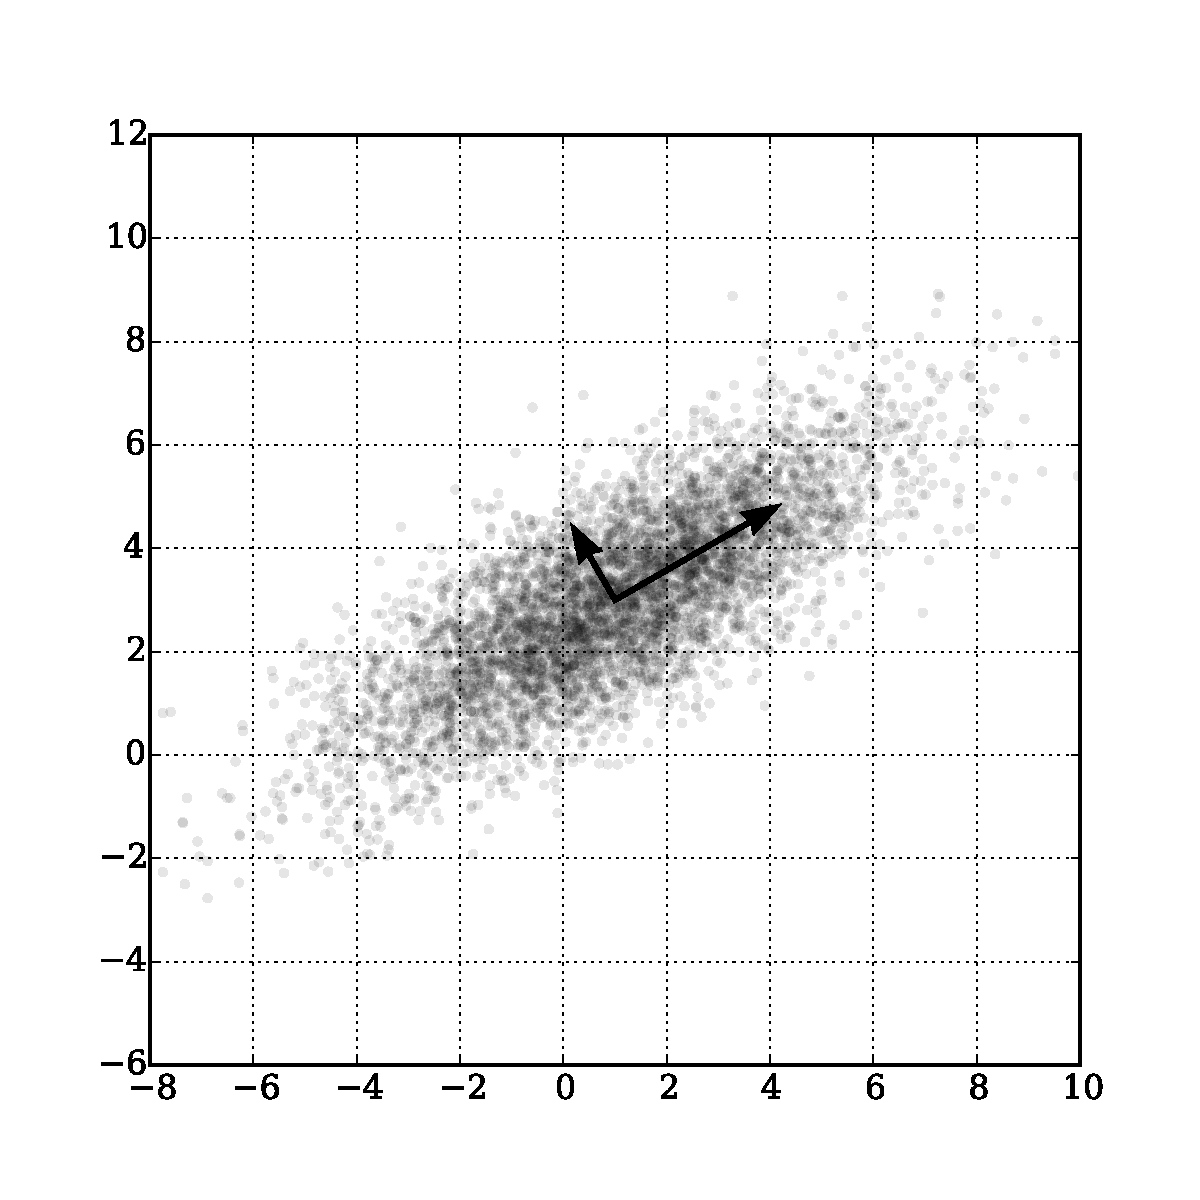
\includegraphics[width=\textwidth]{images/GaussianScatterPCA.pdf}\vspace{-3mm}
      {\tiny [Image from Wikimedia Commons]}}%
      \only<2->{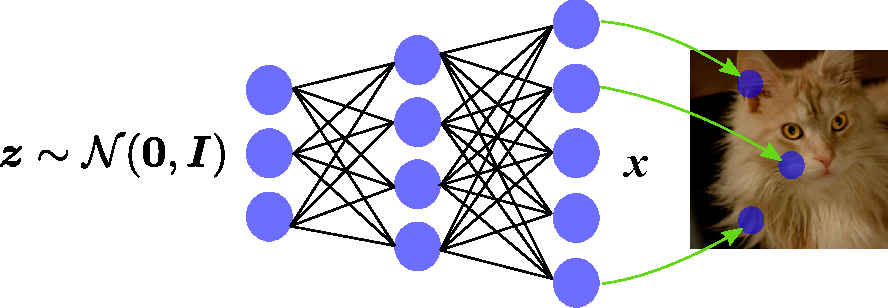
\includegraphics[width=\textwidth]{images/gen_model.pdf}}
   \end{column}
  \end{columns}
  \vspace{-8mm}
\end{frame}

% %%%%%%%%%%%%%%%%%%%%%%%%%%%%%%%%%%%%%%%%%%%%%%%%%%%%%%%%%%%%%%%%%%%%%%%%%%%%
% \begin{frame}{Comments on PPCA - Toward VAE}
% \begin{itemize}
%  \item It is possible to derive an exact EM algorithm $\rightarrow$ local convergence guaranteed.
%  \item Can only model linear dependencies $\rightarrow$ limited expressivity.
% \end{itemize}
%
% Non-linear Gaussian model: $ p_{\bs{\theta}}(\bs{x}|\bs{z})=\mathcal{N}\Big(\bs{x};\bs{\mu}_{\bs{\theta}}(\bs{z}),\bs{\Sigma}_{\bs{\theta}}(\bs{z})\Big) $
% 	\begin{itemize}
% 		\item $ \bs{\mu}_{\bs{\theta}}(.), \bs{\Sigma}_{\bs{\theta}}(.) $: Non-linear functions implemented as deep nets
% 		\item Parameter estimation is challenging, but much more expressive
% 	\end{itemize}
% \begin{figure}
% 	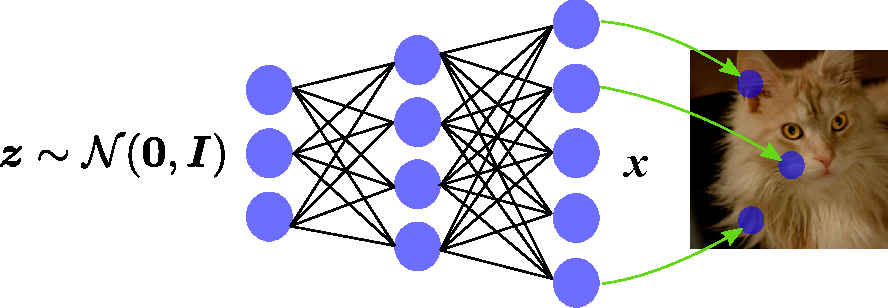
\includegraphics[scale=0.45]{images/gen_model.pdf}
% \end{figure}
%
% The non-linear Gaussian model can be optimised via the variational autoencoder (VAE).
% \end{frame}
%
% %%%%%%%%%%%%%%%%%%%%%%%%%%%%%%%%%%%%%%%%%%%%%%%%%%%%%%%%%%%%%%
% \begin{frame}{Formalising the generative model (I)}
%   How can we ensure that $\bs{\Sigma}_{\bs{\theta}}(\bs{z})$ is a covariance matrix?
%   \begin{itemize}
%    \item The covariance matrix is assumed to be diagonal:
%    \begin{equation*}\bs{\Sigma}_{\bs{\theta}}(\bs{z}) = \left(\begin{array}{cccc}
%    \nu_{\bs{\theta},1}(\bs{z}) & 0 & \cdots & 0 \\
%    0 & \nu_{\bs{\theta},2}(\bs{z}) & \cdots & 0 \\
%    \vdots & \vdots & \ddots & \vdots \\
%    0 & 0 & \cdots & \nu_{\bs{\theta},F}(\bs{z})
%    \end{array}\right)\end{equation*}
%    Reduces complexity and memory, but also expressivity.
%    \item We estimate the log-variance: $\eta_{\bs{\theta},f}(\bs{z}) = \log \nu_{\bs{\theta},f}(\bs{z})$:
%    \begin{equation*}\bs{\Sigma}_{\bs{\theta}}(\bs{z}) = \textrm{diag}_f \left(\exp \left(\eta_{\bs{\theta},f}(\bs{z})\right)\right)\end{equation*}
%    The values of $\eta_{\bs{\theta},f}(\bs{z})$ can be positive or negative.
%   \end{itemize}
%
%
% \end{frame}
%
% %%%%%%%%%%%%%%%%%%%%%%%%%%%%%%%%%%%%%%%%%%%%%%%%%%%%%%%%%%%%%%
% \begin{frame}{Formalising the generative model (II)}
%   In terms of probabilistic dependencies, they are the same as PPCA:\vspace{3mm}\\
%   \begin{tikzpicture}[->]
%    \node[latent,draw] (z)  {$\bs{z}$};
%    \node[latent,draw,right=of z] (x) {$\bs{x}$};
%    \edge{z} {x};
%   \end{tikzpicture}
%
%   But we can also draw the non-lineariry:\vspace{3mm}\\
%   \begin{tikzpicture}[->]
%    \node[latent,draw] (z)  {$\bs{z}$};
%    \node[net,draw,trapezium angle=85,right=of z] (dec) {$\bs{f}_{\bs{\theta}}(\bs{z})=[\bs{\mu}_{\bs{\theta}}(\bs{z}),\bs{\Sigma}_{\bs{\theta}}(\bs{z})]$};
%    \node[latent,draw,right=of dec] (x) {$\bs{x}$};
%    \edge[dashed] {z} {dec};
%    \edge{dec} {x};
%   \end{tikzpicture}\vspace{3mm}
%
%   The dependency of the parameters w.r.t.\ $\bs{z}$ is \textbf{deterministic}.\vspace{3mm}
%
%   Denoted by $\bs{f}_{\bs{\theta}}(\bs{z}):\mathbb{R}^{D}\rightarrow\mathbb{R}^{2F}$, this non-linearity is implemented with a deep network, with parameters (weights and biases) $\bs{\theta}$.
%
% \end{frame}


%%%%%%%%%%%%%%%%%%%%%%%%%%%%%%%%%%%%%%%%%%%%%%%%%%%%%%%%%%%%%%
\begin{frame}{The posterior distribution}
 If $p_{\bs{\theta}}(\bs{x}|\bs{z})$ is non-linear, $p_{\bs{\theta}}(\bs{z}|\bs{x})$ cannot be computed analytically, it needs to be approximated.\vspace{3mm}\\
 
 The idea is to find the \textcolor{myorange}{best candidate within a family of distributions}.\vspace{3mm}\\
 
 \begin{figure}
  \centering
  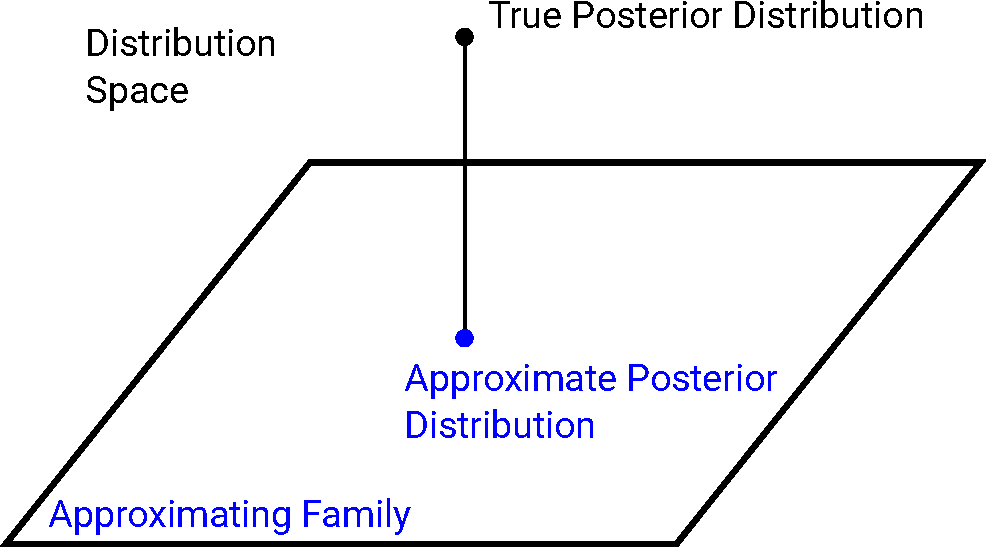
\includegraphics[width=0.56\textwidth]{images/distribution_projection.pdf}
 \end{figure}

\end{frame}
%
% %%%%%%%%%%%%%%%%%%%%%%%%%%%%%%%%%%%%%%%%%%%%%%%%%%%%%%%%%%%%%%
% \begin{frame}{Approximating the posterior distribution}
%
%  The posterior distribution will be approximated with \textbf{another} feed-forward network parametrised with $\bs{\phi}$:
%  \begin{equation*}
%  p(\bs{z}|\bs{x})\approx q(\bs{z}|\bs{x}) = \mathcal{N}(\bs{z};\tilde{\bs{\mu}}_{\bs{\phi}}(\bs{x}),\tilde{\bs{\Sigma}}_{\bs{\phi}}(\bs{x}))
%  \end{equation*}
%
%  The approximating family is composed of all the distributions that can be expressed as above, for a certain value of $\bs{\phi}$.
%  \begin{equation*}
%  \mathcal{G} = \{ \bs{g}_{\bs{\phi}}:\mathbb{R}^{F}\rightarrow\mathbb{R}^{2D};\bs{\phi}\in\bs{\Phi} \},
%  \end{equation*}
%  with $\bs{g}_{\bs{\phi}}(\bs{x}) = [\tilde{\bs{\mu}}_{\bs{\phi}}(\bs{x}),\tilde{\bs{\Sigma}}_{\bs{\phi}}(\bs{x})]$.
% \end{frame}

%%%%%%%%%%%%%%%%%%%%%%%%%%%%%%%%%%%%%%%%%%%%%%%%%%%%%%%%%%%%%%
\begin{frame}{Overall architecture}
 If we ``chain'' the posterior (encoder) and the generative (decoder) model:\vspace{3mm}
   \begin{figure}
    \centering
    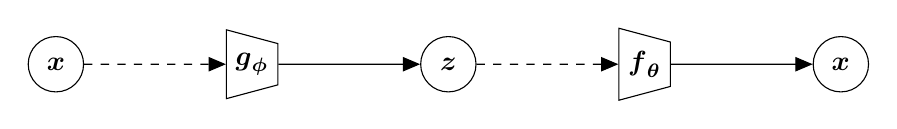
\begin{tikzpicture}[->]
    \node[latent,draw] (xi) {$\bs{x}$};
    \node[net,draw,right=1.8cm of xi] (enc) {$\bs{g}_{\bs{\phi}}$};
    \node[latent,draw,right=1.8cm of enc] (z)  {$\bs{z}$};
    \node[net,draw,right=1.8cm of z] (dec) {$\bs{f}_{\bs{\theta}}$};
    \node[latent,draw,right=1.8cm of dec] (x) {$\bs{x}$};
    \edge[dashed] {xi} {enc};
    \edge{enc} {z};
    \edge[dashed] {z} {dec};
    \edge{dec} {x};
    \end{tikzpicture}\\
    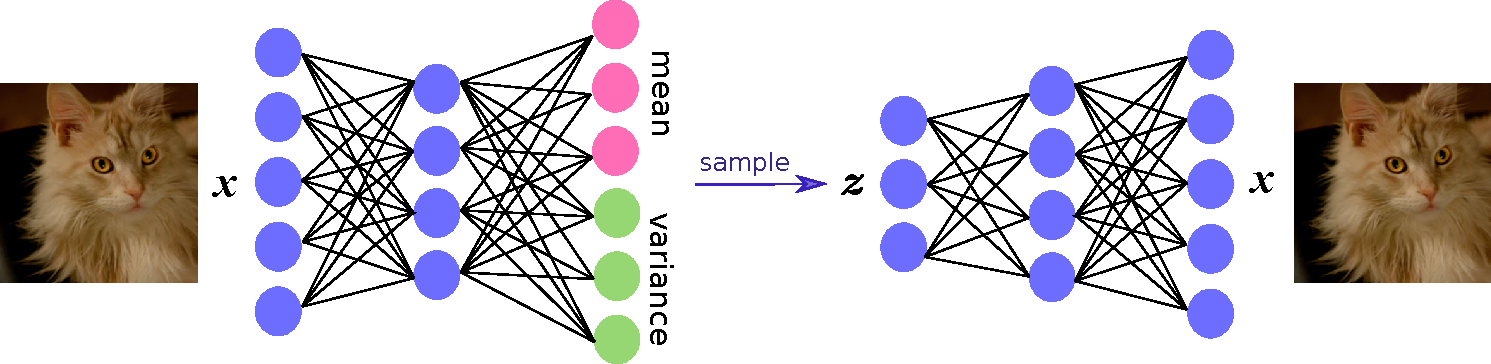
\includegraphics[width=0.8\textwidth]{images/geninf_model.pdf}
   \end{figure}
\begin{center}
 $ p(\bs{z}|\bs{x})\approx q(\bs{z}|\bs{x}) = \mathcal{N}\Big(\bs{z};\tilde{\bs{\mu}}_{\bs{\phi}}(\bs{x}),\tilde{\bs{\Sigma}}_{\bs{\phi}}(\bs{x})\Big) \qquad p_{\bs{\theta}}(\bs{x}|\bs{z}) =\mathcal{N}\Big(\bs{x};\bs{\mu}_{\bs{\theta}}(\bs{z}),\bs{\Sigma}_{\bs{\theta}}(\bs{z})\Big)$
\end{center}



%  This is why we call these architectures \textbf{variational autoencoders} VAE.\vspace{3mm}
 
 But how do we optimise for the parameters $\bs{\theta}$ and $\bs{\phi}$?

\end{frame}

%%%%%%%%%%%%%%%%%%%%%%%%%%%%%%%%%%%%%%%%%%%%%%%%%%%%%%%%%%%%%%
\begin{frame}{Learning - ELBO}
 If we recall the formulation for the EM:
 \begin{align*}
\log p(\bs{x}) &= \mathbb{E}_{q(\bs{z}|\bs{x})}\Big[\log \frac{p(\bs{x},\bs{z})}{q(\bs{z}|\bs{x})}\Big] + {\color{red} D_{\text{KL}}\Big(q(\bs{z}|\bs{x})\Big\lVert p(\bs{z}|\bs{x})\Big)}
\end{align*}\pause
Problem: the second term cannot be computed! But it's positive:
 \begin{align*}
\log p(\bs{x};\bs{\theta},\bs{\phi}) &\; {\color{red}\geq}\; {\color{blue} \mathbb{E}_{q_{\bs{\phi}}(\bs{z}|\bs{x})}\Big[\log \frac{p(\bs{x},\bs{z})}{q_{\bs{\phi}}(\bs{z}|\bs{x})}\Big]} \\
\log p(\bs{x};\bs{\theta},\bs{\phi}) &\; {\color{red}\geq}\; {\color{blue} \underbrace{\mathbb{E}_{q_{\bs{\phi}}(\bs{z}|\bs{x})}\Big[\log p_{\bs{\theta}}(\bs{x}|\bs{z})\Big]}_{\text{Reconstruction}} -  \underbrace{D_{\text{KL}}\Big(q_{\bs{\phi}}(\bs{z}|\bs{x})\Big\lVert p(\bs{z})\Big)}_{\text{Regularisation}}}
\end{align*}
This is known as \textbf{Evidence Lower-BOund or ELBO}: $\mathcal{L}_{\text{ELBO}}(\bs{\theta},\bs{\phi})$.\vspace{3mm}\\
Be VERY careful with these expressions: They look alike, but they are NOT the same.
\end{frame}

%%%%%%%%%%%%%%%%%%%%%%%%%%%%%%%%%%%%%%%%%%%%%%%%%%%%%%%%%%%%%%
\begin{frame}{Learning - Practical comments}
\begin{align*}
\log p(\bs{x}) &\geq \mathbb{E}_{q(\bs{z}|\bs{x})}\Big[\log \frac{p(\bs{x},\bs{z})}{q(\bs{z}|\bs{x})}\Big] = \mathcal{L}_{\text{ELBO}}(\bs{\theta},\bs{\phi})
\end{align*}

\begin{itemize}
\item One needs to sample from $q(\bs{z}|\bs{x})$ to compute the expectation.
\item This sampling needs the ``reparametrisation trick'' to be differentiable.
\item Most libraries solve a minimisation problem $\rightarrow$ we need to provide $-\mathcal{L}_{\text{ELBO}}(\bs{\theta},\bs{\phi})$.
\end{itemize}

\end{frame}

%
% %%%%%%%%%%%%%%%%%%%%%%%%%%%%%%%%%%%%%%%%%%%%%%%%%%%%%%%%%%%%%%
% \begin{frame}{Learning - Sampling}
%  But we still have one problem:
%  \begin{align*}
%   \mathcal{L}_{\text{ELBO}}(\bs{\theta},\bs{\phi}) &= \underbrace{\mathbb{E}_{q_{\bs{\phi}}(\bs{z}|\bs{x})}\Big\{\log p_{\bs{\theta}}(\bs{x}|\bs{z})\Big\}}_{\text{Reconstruction}} -  \underbrace{D_{\text{KL}}\Big(q_{\bs{\phi}}(\bs{z}|\bs{x})\Big\lVert p(\bs{z})\Big)}_{\text{Regularisation}}
% \end{align*}
% To compute the ``reconstruction'' term we need to take the expectation w.r.t.\ $q_{\bs{\phi}}(\bs{z}|\bs{x})$, but recall that:
% \begin{equation*}
%   p_{\bs{\theta}}(\bs{x}|\bs{z}) = \mathcal{N}(\bs{x};\bs{\mu}_{\bs{\theta}}(\bs{z}),\bs{\Sigma}_{\bs{\theta}}(\bs{z})).
% \end{equation*}
% Due to the non-linearity, we cannot compute the reconstruction term in closed form\\ $\rightarrow$ we sample $R$ points $\hat{\bs{z}}^{(1)},\ldots,\hat{\bs{z}}^{(R)}$ from $q_{\bs{\phi}}$:
%  \begin{align*}
%   \mathcal{L}_{\text{ELBO}}(\bs{\theta},\bs{\phi}) &= \underbrace{\frac{1}{R}\sum_{r=1}^R\log p_{\bs{\theta}}(\bs{x}|\hat{\bs{z}}^{(r)})}_{\text{Reconstruction}} -  \underbrace{D_{\text{KL}}\Big(q_{\bs{\phi}}(\bs{z}|\bs{x})\Big\lVert p(\bs{z})\Big)}_{\text{Regularisation}}
% \end{align*}
% \end{frame}
%
% %%%%%%%%%%%%%%%%%%%%%%%%%%%%%%%%%%%%%%%%%%%%%%%%%%%%%%%%%%%%%%
% \begin{frame}{Learning - Gradient ascent?}
%   Let's go back to the architecture:\vspace{-3mm}
% \begin{figure}
%   \centering
%    \begin{tikzpicture}[->]
%    \node[latent,draw] (xi) {$\bs{x}$};
%    \node[net,draw,right=of xi] (enc) {$\bs{g}_{\bs{\phi}}$};
%    \node[latent,draw,right=of enc] (z)  {$\hat{\bs{z}}^{(r)}$};
%    \node[net,draw,right=of z] (dec) {$\bs{f}_{\bs{\theta}}$};
%    \node[latent,draw,right=of dec] (x) {$\bs{x}$};
%    \edge[dashed] {xi} {enc};
%    \edge[dotted,thick,red] {enc} {z};
%    \edge[dashed] {z} {dec};
%    \edge{dec} {x};
%   \end{tikzpicture}
%   \end{figure}\vspace{-3mm}
%
%   Since there is no closed-form solution for the parameters (due to the non-linearity), we will learn the parameters using stochastic gradient ascent (to maximise the ELBO).\vspace{3mm}
%
%   We assume that $\bs{g}_{\bs{\phi}}$ and $\bs{f}_{\bs{\theta}}$ are differentiable (we can compute the gradient).\vspace{3mm}
%
%   The sampling operation ($\hat{\bs{z}}^{(r)}$) from $q_{\bs{\phi}}$ is {\color{red}NOT} differentiable w.r.t.\ $\bs{\phi}$.
% \end{frame}
%
% %%%%%%%%%%%%%%%%%%%%%%%%%%%%%%%%%%%%%%%%%%%%%%%%%%%%%%%%%%%%%%
% \begin{frame}{Learning - Reparametrisation trick}
% %  We use the so-called \textbf{reparametrisation trick}:\vspace{3mm}\\
%   Instead of sampling directly from the posterior ($\hat{\bs{z}}^{(r)}\sim q_{\bs{\phi}}=\mathcal{N}(\tilde{\bs{\mu}}_{\bs{\phi}},\tilde{\bs{\Sigma}}_{\bs{\phi}})$) we sample as follows:
%   \begin{equation*}
%    \bar{\bs{z}}^{(r)} = \tilde{\bs{\Sigma}}_{\bs{\phi}}^{1/2} \bar{\bs{\epsilon}}^{(r)} + \tilde{\bs{\mu}}_{\bs{\phi}} \quad\text{with}\quad \bar{\bs{\epsilon}}^{(r)}\sim \mathcal{N}(\bs{0},\bs{I})
%   \end{equation*}
%
%   $\hat{\bs{z}}^{(r)}$ and $\bar{\bs{z}}^{(r)}$ follow the same distribution, BUT $\bar{\bs{z}}^{(r)}$ is differentiable w.r.t.\ $\bs{\phi}$!!!\vspace{3mm}\\\pause
%
%   This is called the \textbf{reparametrisation trick} and can be used with other distributions.\vspace{-3mm}
%   \begin{figure}
%   \centering
%     \begin{tikzpicture}[->]
%    \node[latent,draw] (xi) {$\bs{x}$};
%    \node[net,draw,right=of xi] (enc) {$\bs{g}_{\bs{\phi}}$};
%    \node[latent,draw,right=of enc] (z)  {$\bar{\bs{z}}^{(r)}$};
%    \node[net,draw,right=of z] (dec) {$\bs{f}_{\bs{\theta}}$};
%    \node[latent,draw,right=of dec] (x) {$\bs{x}$};
%    \node[draw,above=of z,yshift=-4mm] (standard) {$\mathcal{N}(\bs{0},\bs{I})$};
%    \edge[dashed] {xi} {enc};
%    \edge[dashed] {enc} {z};
%    \edge[dotted,thick,red] {standard} {z};
%    \edge[dashed] {z} {dec};
%    \edge{dec} {x};
%   \end{tikzpicture}
%   \end{figure}\vspace{-3mm}
% \end{frame}
%
% %%%%%%%%%%%%%%%%%%%%%%%%%%%%%%%%%%%%%%%%%%%%%%%%%%%%%%%%%%%%%%
% \begin{frame}{Learning - Reparametrisation trick (II)}
%  \begin{figure}
%   \centering
%   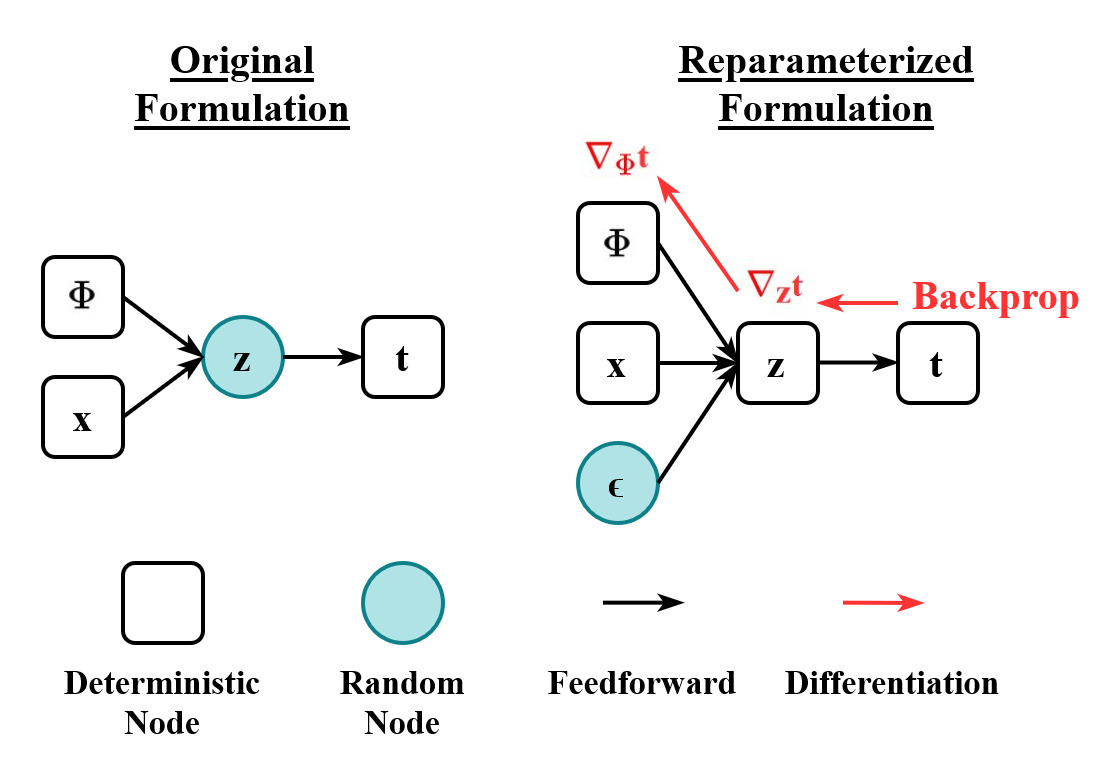
\includegraphics[width=0.5\textwidth]{images/ReparameterizationTrick.jpg}\vspace{-3mm}\\
%   {\tiny [Image from Wikimedia Commons]}
%  \end{figure}
%
% \end{frame}
%
% %%%%%%%%%%%%%%%%%%%%%%%%%%%%%%%%%%%%%%%%%%%%%%%%%%%%%%%%%%%%%%
% \begin{frame}{Training VAE}
%  \textbf{Implementation note}: Most deep learning libraries implement stochastic gradient DESCENT algorithms, but we would like to maximize the ELBO $\rightarrow$ we need to change the sign.\pause
%
%  \textbf{Posterior collapse}: common phenomenon when the posterior $q_{\bs{\phi}}$ gets to close to the standard prior. It can happen for various dimensions of $\bs{z}$ $\rightarrow$ the VAE stops learning.
%  \begin{itemize}
%   \item The KL term dominates the ELBO $\rightarrow$ weight the KL term with $\beta<1$.
%   \item The data can be reduced to less dimensions than $D$ $\rightarrow$ decrease $D$.
%  \end{itemize}
%
% \end{frame}
%
%
% %%%%%%%%%%%%%%%%%%%%%%%%%%%%%%%%%%%%%%%%%%%%%%%%%%%%%%%%%%%%%%%%%%%%%%%%%%%%
% \begin{frame}{VAE: Summary}
% \textbf{Generative model}. Prior:
% 	$p(\bs{z})=\mathcal{N}(\bs{z};\boldsymbol{0},\bs{I})$ and decoder: $p_{\bs{\theta}}(\bs{x}|\bs{z})=\mathcal{N}\Big(\bs{x};\bs{\mu}_{\bs{\theta}}(\bs{z}),\bs{\Sigma}_{\bs{\theta}}(\bs{z})\Big)$.
%
% \textbf{Inference model} (encoder): $p_{\bs{\theta}}(\bs{z}|\bs{x}) \approx q_{\bs{\phi}}(\bs{z}|\bs{x})=\mathcal{N}\Big(\bs{z};\bs{\mu}_{\bs{\phi}}(\bs{x}),\bs{\Sigma}_{\bs{\phi}}(\bs{x})\Big)$
% \begin{figure}
% 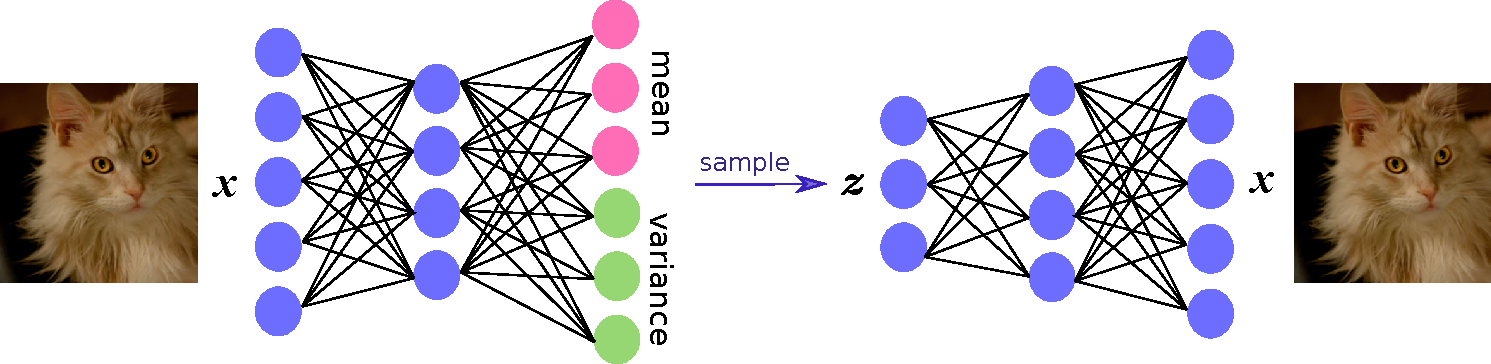
\includegraphics[scale=0.4]{images/geninf_model.pdf}
% \end{figure}
% \textbf{Training criterion} (maximise the evidence lower bound):
%  \begin{align*}
%   \mathcal{L}_{\text{ELBO}}(\bs{\theta},\bs{\phi}) &= \underbrace{\log p_{\bs{\theta}}(\bs{x}|\hat{\bs{z}})}_{\text{Reconstruction}} -  \underbrace{D_{\text{KL}}\Big(q_{\bs{\phi}}(\bs{z}|\bs{x})\Big\lVert p(\bs{z})\Big)}_{\text{Regularisation}}
% \end{align*}
% 	where $\hat{\bs{z}}\sim q_{\bs{\phi}}$ is sampled using the reparametrisation trick.
% \end{frame}

%%%%%%%%%%%%%%%%%%%%%%%%%%%%%%%%%%%%%%%%%%%%%%%%%%%%%%%%%%%%%%%%%%%%%%%%%%%%
\begin{frame}{ML with latent variables: EM vs VAE?}
ML with latent variable ($\bs{z}$) leads to EM\footnote{Dempster, A.P., \textit{et. al.}, (1977), Journal of the Royal Statistical Society.} and VI\footnote{Jordan, M. I., \textit{et. al.}, (1999),. Machine Learning.} build from {\footnotesize($\color{blue}q(\bs{z})$ is an arbitrary distribution)}:
\begin{align*}
\log p(\bs{x}) &= \underbrace{\mathbb{E}_{\color{blue}q(\bs{z})}\Big[\log \frac{p(\bs{x})p(\bs{z}|\bs{x})}{\color{blue}q(\bs{z})}\Big]}_{\text{M-step or VLB}} +  \underbrace{D_{\text{KL}}\Big({\color{blue}q(\bs{z})}\Big\lVert p(\bs{z}|\bs{x})\Big)}_{\text{E-step}}
\end{align*}
\begin{columns}
 \begin{column}{0.31\textwidth}
  \centering
  \underline{Exact EM}\\
  Simple $p(\bs{z}|\bs{x})$ \\
  ${\color{blue}q(\bs{z})}=p(\bs{z}|\bs{x})$\\
  Closed-form!\\
  $D_{\text{KL}} = 0$
 \end{column}\visible<2>{%
 \begin{column}{0.31\textwidth}
 \centering
  \underline{Variational EM}\\
  $p(\bs{z}|\bs{x})$ comp. complex\\
  ${\color{myorange}q([\bs{z}_1,\bs{z}_2]) = q_1(\bs{z}_1)q_2(\bs{z}_2)}$\\
  $q_1,q_2=\argmin D_{\text{KL}}$\\
  $D_{\text{KL}}>0$ but closed form!
 \end{column}}%
  \begin{column}{0.31\textwidth}
 \centering
  \underline{Variational AutoEncoder}\\
  $p(\bs{z}|\bs{x})$ ???\\
  ${\color{blue}q(\bs{z})} = q_{\bs{\phi}}(\bs{z})$\\
  $q_{\bs{\phi}}$ optimises ELBO/VLB\\
  $D_{\text{KL}}>0$ no closed form!
 \end{column}
\end{columns}
\end{frame}

%%%%%%%%%%%%%%%%%%%%%%%%%%%%%%%%%%%%%%%%%%%%%%%%%%%%%%%%%%%%%%%%%%%%%%%%%%%%
%%%%%%%%%%%%%%%%%%%%%%%%%%%%%%%%%%%%%%%%%%%%%%%%%%%%%%%%%%%%%%%%%%%%%%%%%%%%
{\setbeamercolor{background canvas}{bg=mDarkTeal}
\setbeamercolor{background canvas}{fg=white}
\begin{frame}
 \centering
 \color{white}\large\bf Audio-Visual Unsupervised Speech Enhancement with VAEs \vspace{1cm}

 \begin{columns}
 \begin{column}{3cm}
    \centering
    \includegraphics[width=.66\textwidth]{people/mostafa.png}\\
    \color{white}Mostafa Sadeghi
 \end{column}
 \begin{column}{3cm}
    \centering
    \includegraphics[width=.66\textwidth]{people/laurent.png}\\
    \color{white}Laurent Girin
 \end{column}
 \begin{column}{3cm}
    \centering
    \includegraphics[width=.66\textwidth]{people/radu.png}\\
    \color{white}Radu Horaud
 \end{column}
\end{columns}
\end{frame}}

%%%%%%%%%%%%%%%%%%%%%%%%%%%%%%%%%%%%%%%%%%%%%%%%%%%%%%%%%%%%%%%%%%%%%%%%%%%%
\begin{frame}{Speech Enhancement \& Wiener Filter}
 \begin{columns}
 \begin{column}{0.48\textwidth}
  \begin{figure}
\centering
    \includegraphics[height=3cm]{images/intro_speech_enhancement_v2.pdf}
  \end{figure}
 \end{column}%
 \begin{column}{0.48\textwidth}
 \centering
 \only<2>{Minimize MSE $\rightarrow$ Wiener Filter\\
 {\footnotesize (operations are element-wise)}\vspace{-5mm}\\
 \begin{equation*}
   {\color{red}\hat{\bs{s}}} = \frac{\color{red}{\bs{\sigma}_{\bs{s}}}}{{\color{red}{\bs{\sigma}_{\bs{s}}}} + \color{gray}{\bs{\sigma}_{\bs{b}}}} {\color{green}\bs{x}}
 \end{equation*}
}
 \end{column}
\end{columns}
Extract the \textcolor{red}{latent clean speech signal} from the \textcolor{green}{observed noisy mixture}. (STFT domain)
\begin{figure}
\centering
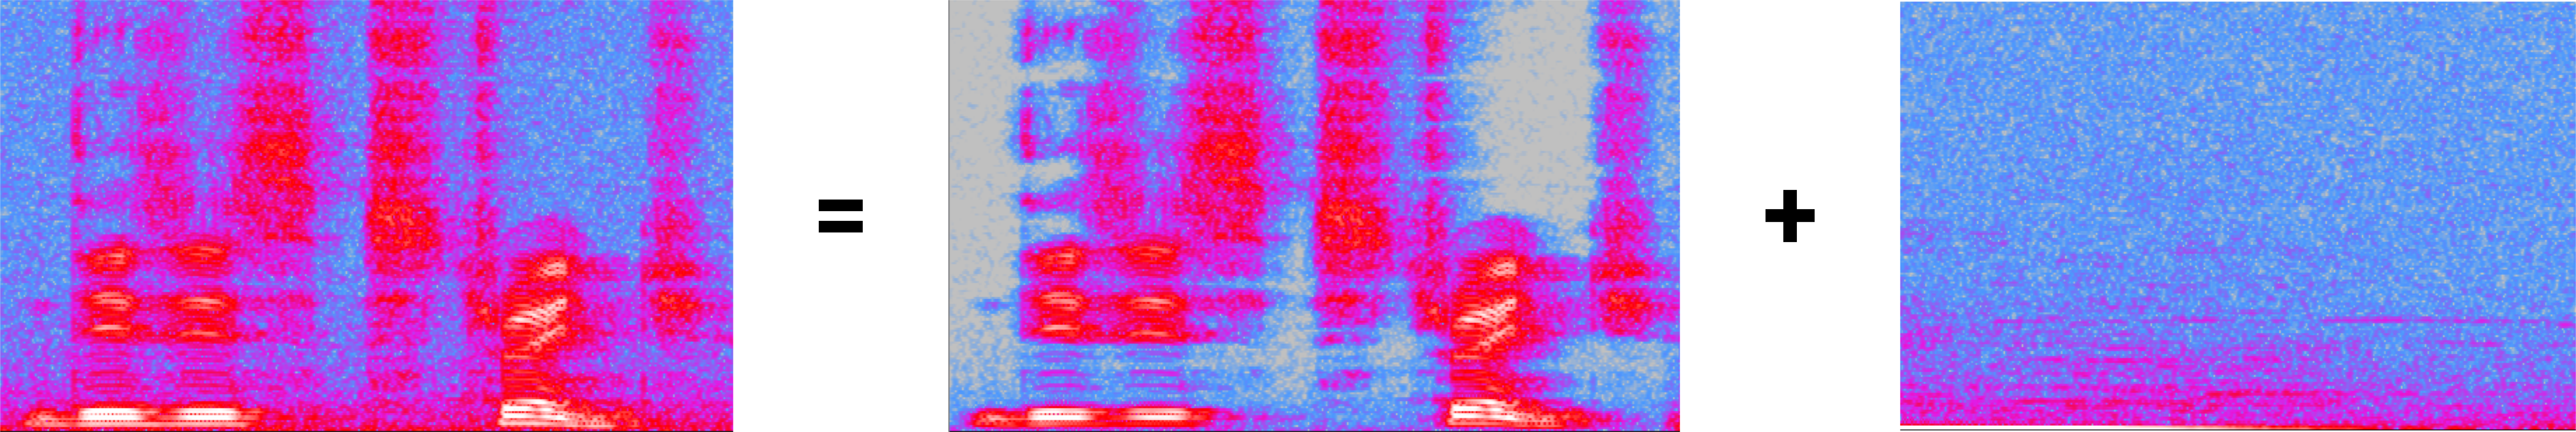
\includegraphics[width=0.8\textwidth]{images/spectrogram.png}
\end{figure}
\vspace{-1mm}
\begin{equation*}
{\color{red}\underbrace{\mathbf{s}}_{\text{Clean speech}}} \quad\qquad+\quad\qquad {\color{gray}\underbrace{\mathbf{b}}_{\text{Noise signal}}}  \quad\qquad=\quad\qquad {\color{green}\underbrace{\mathbf{x}}_{\text{Noisy mixture}}}
\end{equation*}
\end{frame}

%%%%%%%%%%%%%%%%%%%%%%%%%%%%%%%%%%%%%%%%%%%%%%%%%%%%%%%%%%%%%%%%%%%%%%%%%%%%
\begin{frame}{Representing audio: time \textit{vs}. frequency}
 Fourier domain decomposes the signal in frequencies:\\
 \begin{figure}
  \centering
  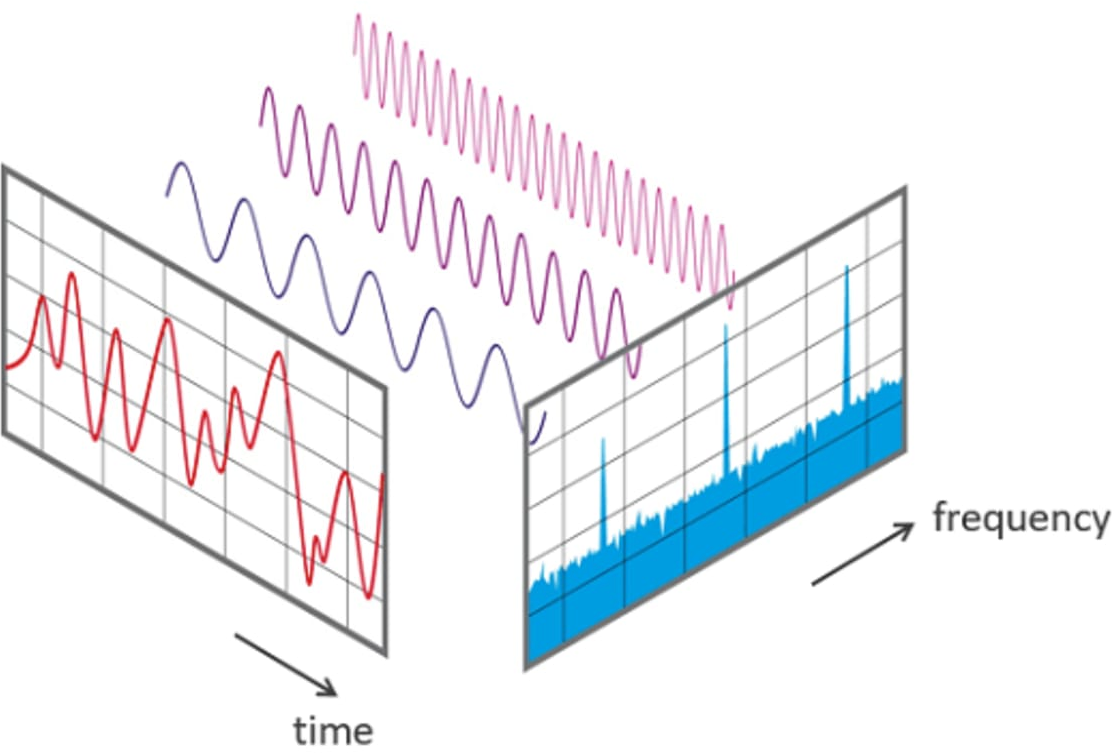
\includegraphics[width=0.6\textwidth]{images/fourierdomain.png}\vspace{-3mm}\\
  {\tiny [Image from \url{https://dev.to/trekhleb/}]}
 \end{figure}
 Problem: we have to choose either time \textbf{or} frequency.
\end{frame}

%%%%%%%%%%%%%%%%%%%%%%%%%%%%%%%%%%%%%%%%%%%%%%%%%%%%%%%%%%%%%%%%%%%%%%%%%%%%
\begin{frame}{The short-time Fourier transform (STFT)}
 STFT: segment the input signal, and apply DFT to each segment.
\begin{figure}
\centering
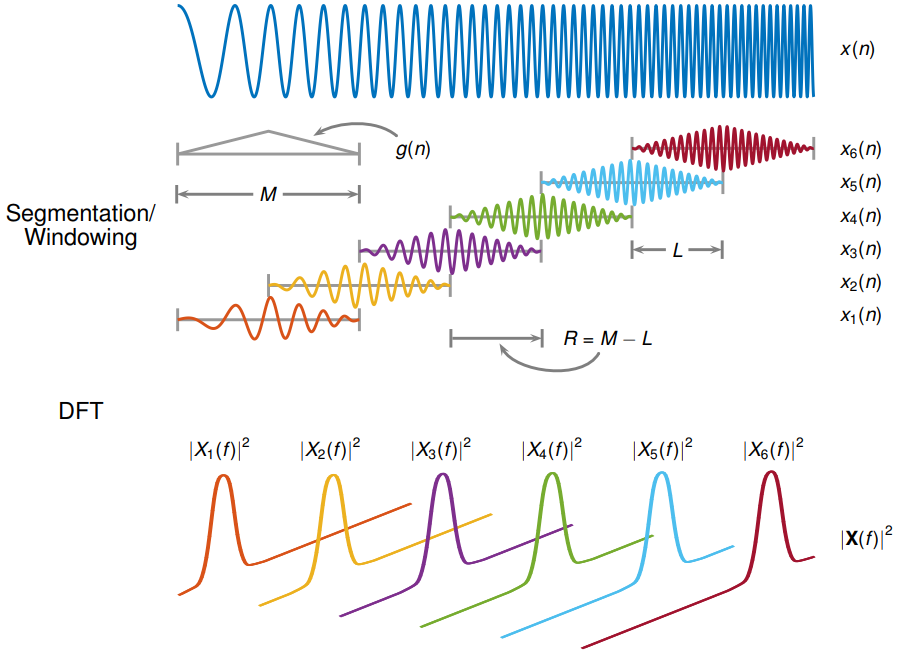
\includegraphics[width=0.55\textwidth]{images/stft.png}\vspace{-3mm}\\
  {\tiny [Image from Mathworks]}
\end{figure}
\end{frame}

%%%%%%%%%%%%%%%%%%%%%%%%%%%%%%%%%%%%%%%%%%%%%%%%%%%%%%%%%%%%%%%%%%%%%%%%%%%%
\begin{frame}{Let's see it!}
\begin{itemize}
 \item Sine frequency sweep (pure sine of increasing frequency).
 \item Leyenda (piano, harmonics).
 \item O mio babbino caro (opera, vibrato).
 \item A few good men (speech, separation).
 \item ...
\end{itemize}
\end{frame}

%%%%%%%%%%%%%%%%%%%%%%%%%%%%%%%%%%%%%%%%%%%%%%%%%%%%%%%%%%%%%%%%%%%%%%%%%%%%
\begin{frame}{Unsupervised Probabilistic SE: paradigm}
\begin{figure}
\centering
\only<1>{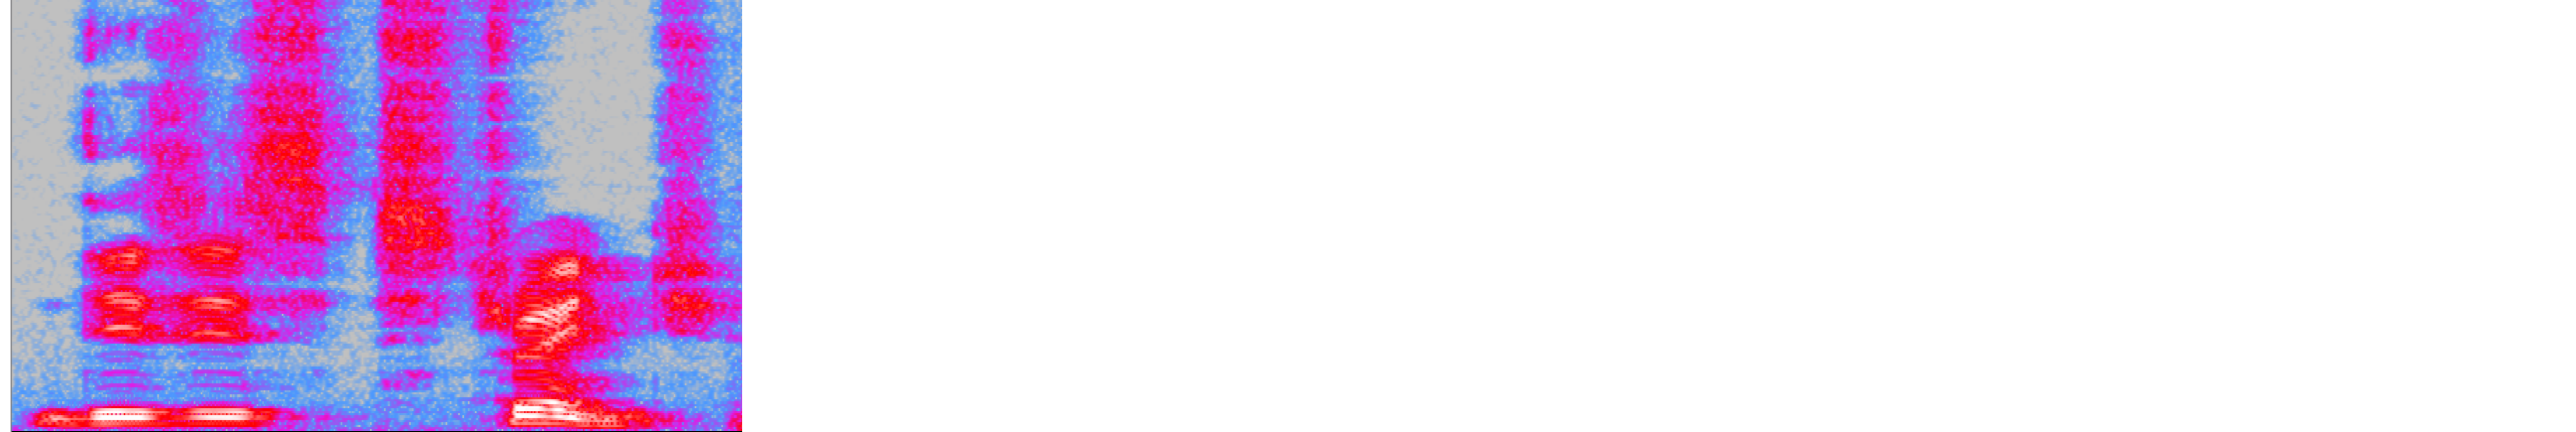
\includegraphics[width=0.8\textwidth]{images/spectrogram_cut.png}}%
\only<2>{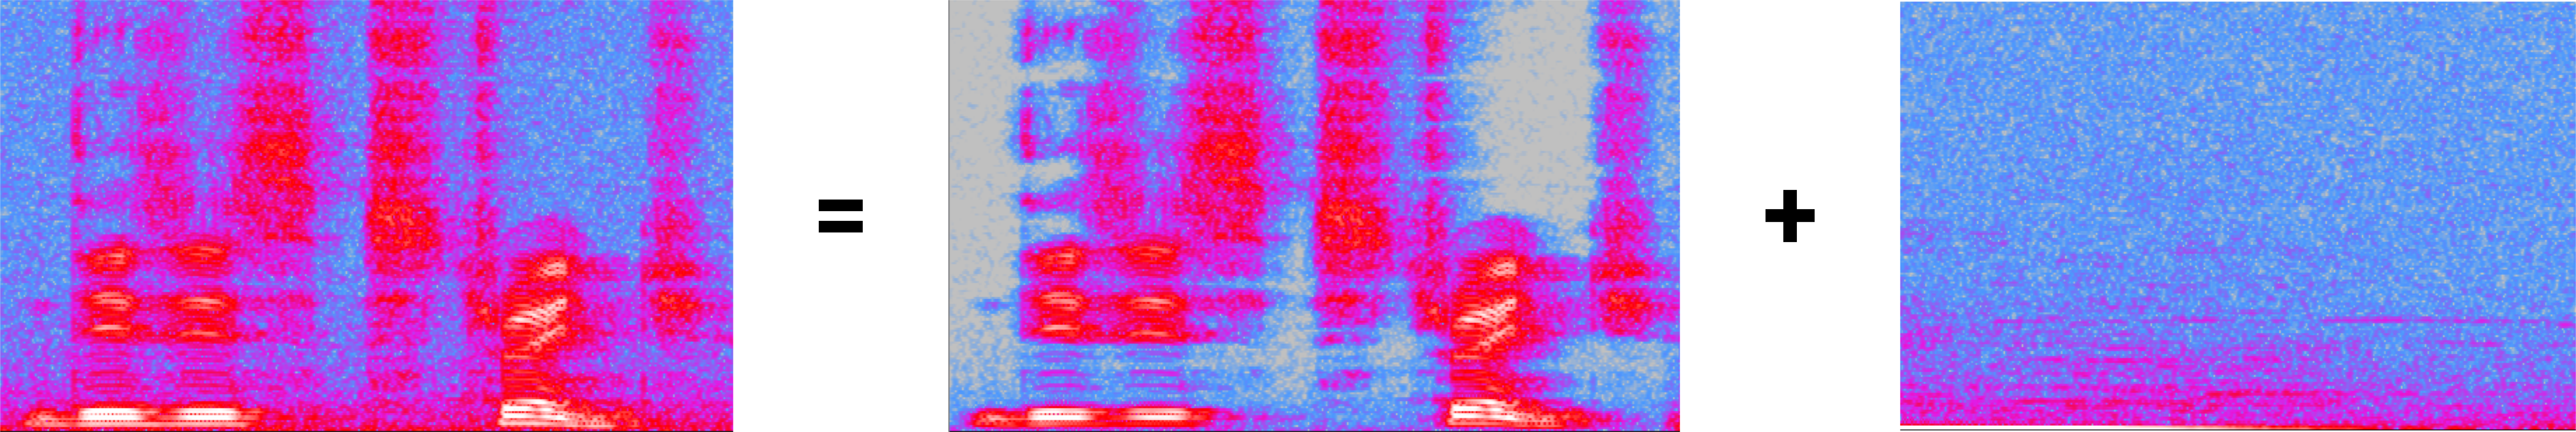
\includegraphics[width=0.8\textwidth]{images/spectrogram.png}}
\end{figure}
\vspace{-6mm}
\begin{equation*}
\only<1>{{\color{green}\underbrace{\mathbf{s}}_{\text{Clean speech}}} {\color{white}\quad\qquad+\quad\qquad \underbrace{\mathbf{b}}_{\text{Noise signal}}  \quad\qquad=\quad\qquad {\underbrace{\mathbf{x}}_{\text{Noisy mixture}}}}}
\only<2>{{\color{red}\underbrace{\mathbf{s}}_{\text{Clean speech}}} \quad\qquad+\quad\qquad {\color{gray}\underbrace{\mathbf{b}}_{\text{Noise signal}}}  \quad\qquad=\quad\qquad {\color{green}\underbrace{\mathbf{x}}_{\text{Noisy mixture}}}}
\end{equation*}

\begin{columns}
 \begin{column}{0.5\textwidth}
  \alert<1>{\textbf{Train}} -- Model for \textcolor<1>{green}{clean data}: $\{{\only<1>{\color{green}}\bs{s}_i}\}_{i=1}^N$.
    \begin{center}
    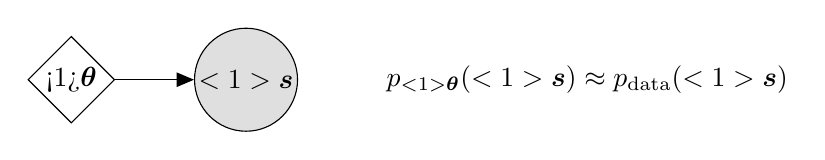
\begin{tikzpicture}
            \node[det] (theta) {\alert<1>{$\bs{\theta}$}};
            \node[obs,right=of theta] (s) {$\only<1>{\color{green}}\bs{s}$};
            \node[right=of s] (disc) {$p_{\alert<1>{\bs{\theta}}}({\only<1>{\color{green}}\bs{s}})\approx p_{\text{data}}({\only<1>{\color{green}}\bs{s}})$};
            \edge{theta} {s};
    \end{tikzpicture}
    \end{center}
    Then freeze $\alert<1>{\bs{\theta}}$ at test/adaptation time.
 \end{column}\pause
 \begin{column}{0.5\textwidth}
  \textbf{Test} -- learn the \alert{noise parameters} from {\color{green} noisy samples $\mathbf{x}$} and estimate the {\color{red} clean speech $\hat{\bs{s}}$}:
    \begin{center}
    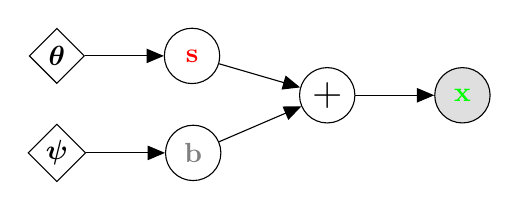
\begin{tikzpicture}
            \node[det] (theta) {$\bs{\theta}$};
            \node[latent,right=of theta] (s) {$\color{red}\mathbf{s}$};
            \node[det,below=of theta,yshift=5mm] (eta) {$\alert{\bs{\psi}}$};
            \node[latent,right=of eta] (b) {$\color{gray}\mathbf{b}$};
            \node[latent,right=of s,yshift=-5mm] (plus) {\Large$+$};
            \node[obs,right=of plus] (x) {$\color{green}\mathbf{x}$};
            \edge{theta} {s};
            \edge{eta} {b};
            \edge{s,b} {plus};
            \edge{plus} {x};
    \end{tikzpicture}
    \end{center}
 \end{column}
\end{columns}

% \textbf{Note}: at test time, $\bs{\theta}$ is frozen, and $\mathbf{s}$ becomes a latent variable.
\end{frame}

%%%%%%%%%%%%%%%%%%%%%%%%%%%%%%%%%%%%%%%%%%%%%%%%%%%%%%%%%%%%%%%%%%%%%%%%%%%%
\begin{frame}{Audio-visual Speech Enhancement (AV-SE)}
\begin{itemize}
	\item Visual data (lip motion) provide \alert{complementary information} about the unknown speech.
	\item For \alert{highly noisy audio recordings}, visual information can be very helpful.
\end{itemize}

\begin{center}
	\begin{figure}
		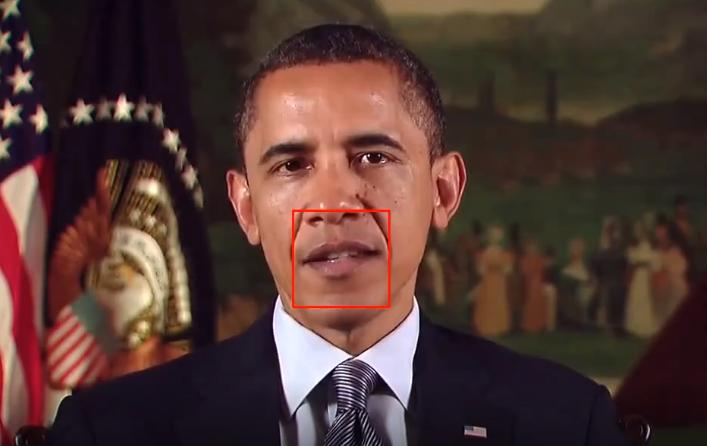
\includegraphics[scale=0.2]{images/obama.png}
	\end{figure}
\end{center}
%\pause
{\small \begin{mybox2}{}
		\centering
		\emph{\small We investigate the VAE framework to fuse audio and visual data for speech enhancement.}
\end{mybox2}}
\end{frame}

%%%%%%%%%%%%%%%%%%%%%%%%%%%%%%%%%%%%%%%%%%%%%%%%%%%%%%%%%%%%%%%%%%%%%%%%%%%%
\begin{frame}{Mono-modal VAEs: the baselines}
\textbf{Audio-only}:\footnote{Leglaive, S., \textit{et. al.}, (2018), IEEE MLSP.}\vspace{-1mm}
\begin{columns}
 \begin{column}{0.5\textwidth}
 \resizebox{\textwidth}{!}{\input{tikz/a_vae.tex}}
%  \includegraphics[width=\textwidth]{images/a_vae_new.pdf}
 \end{column}
 \begin{column}{0.4\textwidth}
 \small
  $p_{\bs{\theta}}(\bs{\myos}_n | \bs{\mylz}_n)= \mathcal{N}_c\Big(\boldsymbol{0}, \text{diag}(\bs{\sigma}_{\myos}(\bs{\mylz}_n))\Big)$\\
  $q_{\bs{\phi}}(\bs{\mylz}_n|\bs{\myos}_n)= \mathcal{N}\Big(\bs{\mu}_{\bs{\mylz}}^a(\bs{\myos}_n), \text{diag}(\bs{\sigma}_{\bs{\mylz}}^a(\bs{\myos}_n))\Big)$
 \end{column}
\end{columns}
\pause
\textbf{Video-only}:
\vspace{-1mm}
\begin{columns}
 \begin{column}{0.5\textwidth}
  \resizebox{\textwidth}{!}{\renewcommand\drawNodes[2]{
  % #1 (str): namespace
  % #2 (list[list[str]]): list of labels to print in the node of each neuron
  \foreach \neurons [count=\lyrIdx] in #2 {
    \StrCount{\neurons}{,}[\lyrLength] % use xstring package to save each layer size into \lyrLength macro

    \ifthenelse{\equal{#1}{encoder}}{
        \ifnumequal{\lyrIdx}{1}
        {% True case
        \foreach \n [count=\nIdx] in \neurons
            \node[neuron,fill=green,fill opacity=0.2] (#1-\lyrIdx-\nIdx) at (0.7*\lyrIdx, \lyrLength/3.6-0.5*\nIdx) {\n};
        }
        {% False case
        \foreach \n [count=\nIdx] in \neurons
            \node[neuron] (#1-\lyrIdx-\nIdx) at (0.7*\lyrIdx, \lyrLength/3.6-0.5*\nIdx) {\n};
        }
    }{
        \ifnumequal{\lyrIdx}{2}
        {% True case
        \foreach \n [count=\nIdx] in \neurons
            \node[neuron,fill=green,fill opacity=0.2] (#1-\lyrIdx-\nIdx) at (0.7*\lyrIdx, \lyrLength/3.6-0.5*\nIdx) {\n};
        }
        {% False case
        \foreach \n [count=\nIdx] in \neurons
            \node[neuron] (#1-\lyrIdx-\nIdx) at (0.7*\lyrIdx, \lyrLength/3.6-0.5*\nIdx) {\n};
        }
    }
  }
}

\renewcommand\denselyConnectNodes[2]{
  % #1 (str): namespace
  % #2 (list[int]): number of nodes in each layer
  \foreach \n [count=\lyrIdx, remember=\lyrIdx as \previdx, remember=\n as \prevn] in #2 {
    \foreach \y in {1,...,\n} {
      \ifnum \lyrIdx > 1
        \foreach \x in {1,...,\prevn}
          \draw[-] (#1-\previdx-\x) -- (#1-\lyrIdx-\y);
      \fi
    }
  }
}

\begin{tikzpicture}[
    shorten >=1pt, shorten <=1pt,
    neuron/.style={circle, draw, minimum size=2ex, thick},
    legend/.style={font=\large\bfseries},
  ]

  % encoder
  \drawNodes{encoder}{{{,,,}, {,,}}}
  \denselyConnectNodes{encoder}{{4, 3}}

  % decoder
  \begin{scope}[xshift=3.7cm]
    \drawNodes{decoder}{{{,,}, {,,,}}}
    \denselyConnectNodes{decoder}{{3, 4}}
  \end{scope}
  
  \node[inner sep=0pt,left of=encoder-1-1,xshift=-0.5cm,yshift=-0.8cm] (input) {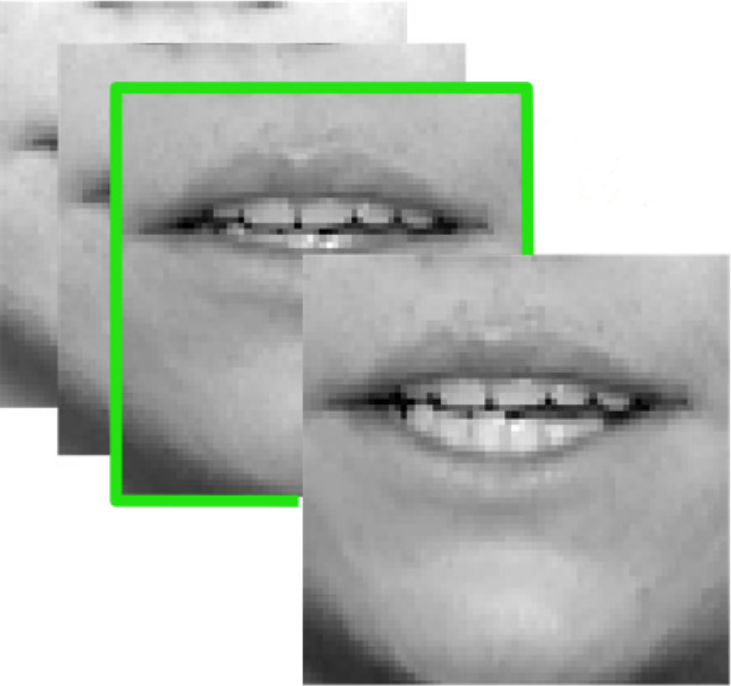
\includegraphics[width=.25\textwidth]{tikz/lips}};
  \node[inner sep=0pt,right of=decoder-2-1,xshift=0.5cm,yshift=-0.8cm] (output) {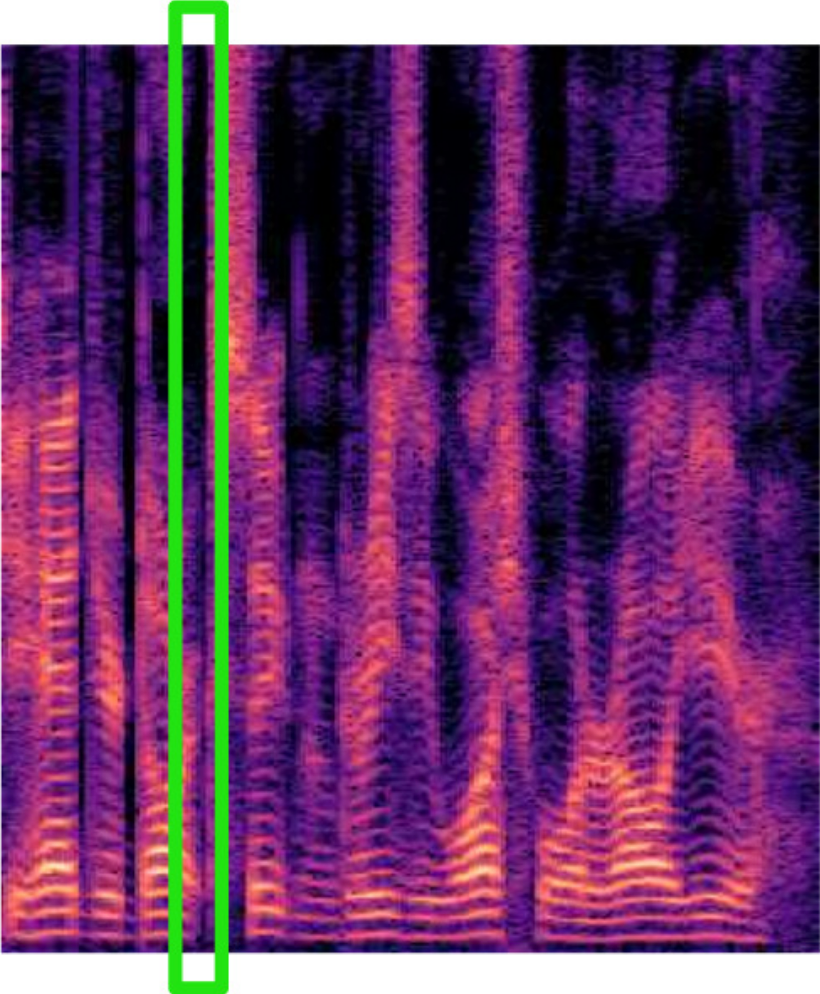
\includegraphics[width=.25\textwidth]{tikz/spectrogram}};
  
  % mu, sigma, sample nodes
  \foreach \idx in {1,...,3} {
      \coordinate[neuron, right=2 of encoder-2-2, xshift=-1.4cm, yshift=0.5*\idx cm-0.15cm, fill=red, fill opacity=0.2] (mu-\idx);
      \coordinate[neuron, right=2 of encoder-2-2, xshift=-1.4cm, yshift=-0.5*\idx cm+0.15cm, fill=red, fill opacity=0.2] (sigma-\idx);
      \coordinate[neuron, right=4 of encoder-2-2, xshift=-2.2cm, yshift=0.5*\idx cm-1cm, fill=red, fill opacity=0.2] (sample-\idx);
    }

  % mu, sigma, sample boxes
  \node [label={above right:$\bs{\mu}^v_{\bs{\mylz}}(\bs{\myov}_n)$}, fit=(mu-1) (mu-3), draw] (mu) {};
  \node [label={below right:$\bs{\sigma}^v_{\bs{\mylz}}(\bs{\myov}_n)$}, fit=(sigma-1) (sigma-3), draw] (sigma) {};
  \node [fit=(sample-1) (sample-3), draw] (sample) {};

  % mu, sigma, sample connections
  \draw[dashed] (mu.east) edge (sample.west) (sigma.east) -- (sample.west);
  \foreach \a in {1,2,3}
  \foreach \b in {1,2,3} {
      \draw[-] (encoder-2-\a) -- (mu-\b);
      \draw[-] (encoder-2-\a) -- (sigma-\b);
      \draw[-] (sample-\a) -- (decoder-1-\b);
    }

  % input + output labels
%   \foreach \idx in {1,...,4} {
%       \node[left=0 of encoder-1-\idx] {$x_\idx$};
%       \node[right=0 of decoder-2-\idx] {$\hat x_\idx$};
%     }
  \node[above=0.1 of encoder-1-1] {$\bs{\myov}_n$};
  \node[above=0.1 of decoder-2-1] {$\hat{\bs{\myos}}_n$};

\end{tikzpicture}
}
%   \includegraphics[width=\textwidth]{images/v_vae_new.pdf}
 \end{column}
 \begin{column}{0.4\textwidth}
 \small
  $p_{\bs{\theta}}(\bs{\myos}_n | \bs{\mylz}_n)= \mathcal{N}_c\Big(\boldsymbol{0}, \text{diag}(\bs{\sigma}_{\myos}(\bs{\mylz}_n))\Big)$\\
  $q_{\bs{\phi}}(\bs{\mylz}_n|\bs{\myov}_n)= \mathcal{N}\Big(\bs{\mu}_{\bs{\mylz}}^v(\bs{\myov}_n), \text{diag}(\bs{\sigma}_{\bs{\mylz}}^v(\bs{\myov}_n))\Big)$
 \end{column}
\end{columns}
\end{frame}

%%%%%%%%%%%%%%%%%%%%%%%%%%%%%%%%%%%%%%%%%%%%%%%%%%%%%%%%%%%%%%%%%%%%%%%%%%%%
\begin{frame}{Audio-visual Conditional VAE\footnote{Sadeghi, M., \textit{et. al.}, (2020), IEEE TASLP.}}
% VAE conditioned with visual frames:\vspace{2mm}
\begin{columns}
 \begin{column}{0.6\textwidth}
 \centering
%  Encoder-Decoder
   \resizebox{\textwidth}{!}{\renewcommand\drawNodes[2]{
  % #1 (str): namespace
  % #2 (list[list[str]]): list of labels to print in the node of each neuron
  \foreach \neurons [count=\lyrIdx] in #2 {
    \StrCount{\neurons}{,}[\lyrLength] % use xstring package to save each layer size into \lyrLength macro

    \ifthenelse{\equal{#1}{encoder}}{
        \ifnumequal{\lyrIdx}{1}
        {% True case
        \foreach \n [count=\nIdx] in \neurons
            \node[neuron,fill=green,fill opacity=0.2] (#1-\lyrIdx-\nIdx) at (0.7*\lyrIdx, \lyrLength/3.6-0.5*\nIdx) {\n};
        }
        {% False case
        \foreach \n [count=\nIdx] in \neurons
            \node[neuron] (#1-\lyrIdx-\nIdx) at (0.7*\lyrIdx, \lyrLength/3.6-0.5*\nIdx) {\n};
        }
    }{
        \ifnumequal{\lyrIdx}{2}
        {% True case
        \foreach \n [count=\nIdx] in \neurons
            \node[neuron,fill=green,fill opacity=0.2] (#1-\lyrIdx-\nIdx) at (0.7*\lyrIdx, \lyrLength/3.6-0.5*\nIdx) {\n};
        }
        {% False case
        \foreach \n [count=\nIdx] in \neurons
            \node[neuron] (#1-\lyrIdx-\nIdx) at (0.7*\lyrIdx, \lyrLength/3.6-0.5*\nIdx) {\n};
        }
    }
  }
}

\renewcommand\denselyConnectNodes[2]{
  % #1 (str): namespace
  % #2 (list[int]): number of nodes in each layer
  \foreach \n [count=\lyrIdx, remember=\lyrIdx as \previdx, remember=\n as \prevn] in #2 {
    \foreach \y in {1,...,\n} {
      \ifnum \lyrIdx > 1
        \foreach \x in {1,...,\prevn}
          \draw[-] (#1-\previdx-\x) -- (#1-\lyrIdx-\y);
      \fi
    }
  }
}

\begin{tikzpicture}[
    shorten >=1pt, shorten <=1pt,
    neuron/.style={circle, draw, minimum size=2ex, thick},
    legend/.style={font=\large\bfseries},
  ]

  % encoder
  \drawNodes{encoder}{{{,,,,,}, {,,}}}
  \denselyConnectNodes{encoder}{{6, 3}}

  % decoder
  \begin{scope}[xshift=3.7cm]
    \drawNodes{decoder}{{{,,}, {,,,}}}
    \denselyConnectNodes{decoder}{{3, 4}}
  \end{scope}
  
  \node[inner sep=0pt,left of=encoder-1-1,xshift=-0.5cm,yshift=-0.2cm] (input) {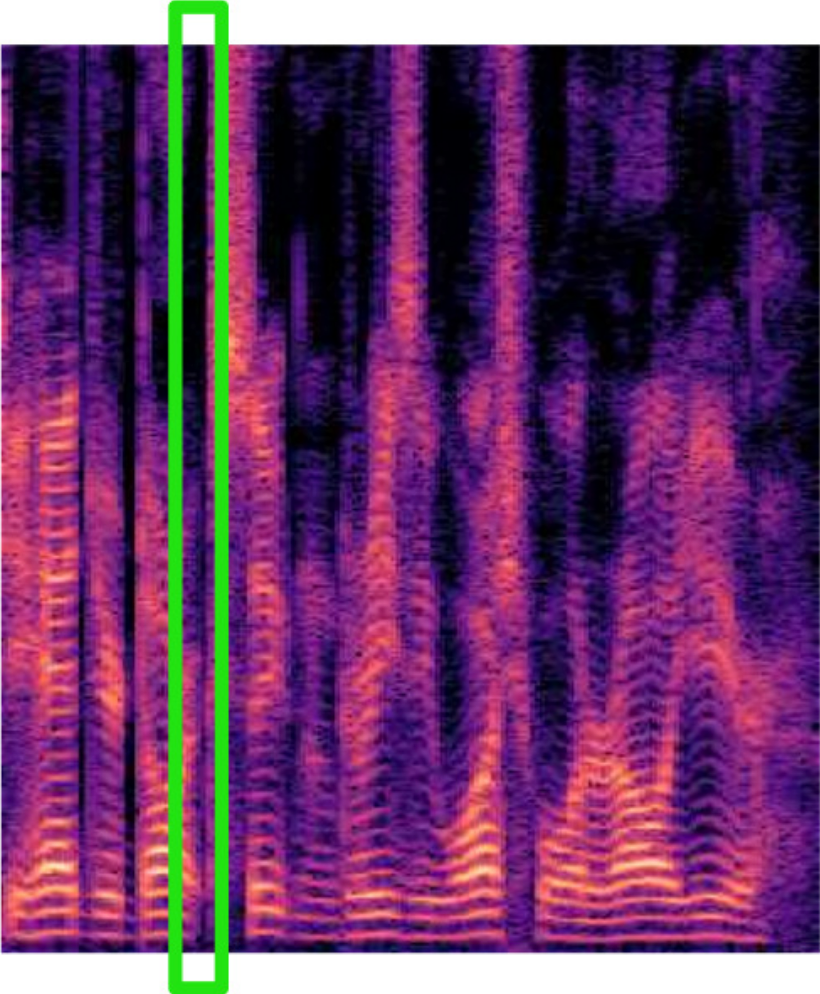
\includegraphics[width=.25\textwidth]{tikz/spectrogram}};
  \node[inner sep=0pt,left of=encoder-1-1,xshift=-0.5cm,yshift=-2.4cm] (input2) {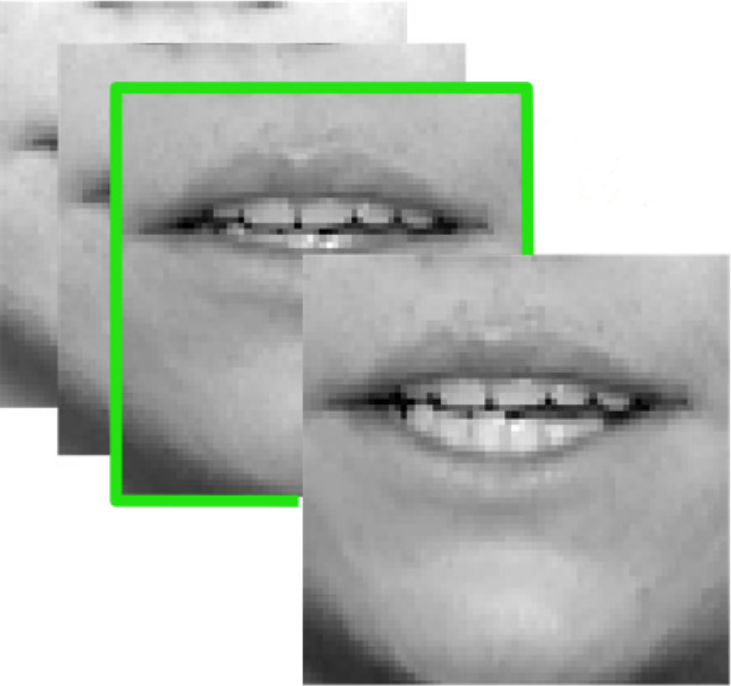
\includegraphics[width=.25\textwidth]{tikz/lips}};
  \node[inner sep=0pt,right of=decoder-2-1,xshift=0.5cm,yshift=-0.8cm] (output) {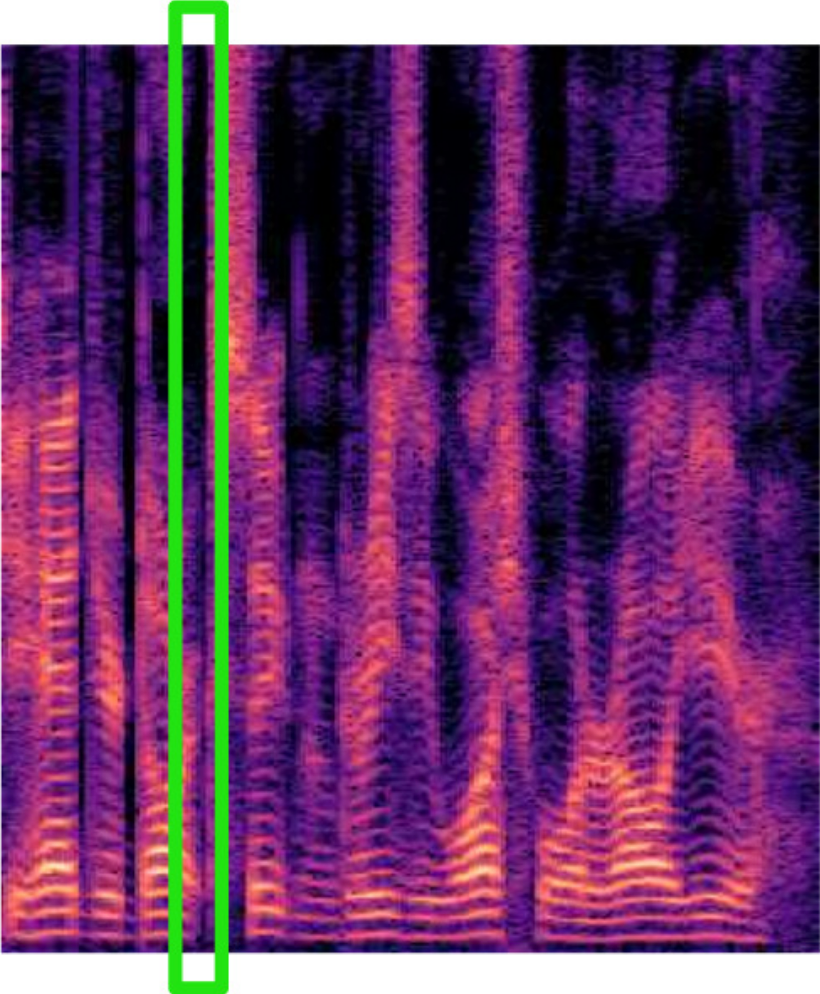
\includegraphics[width=.25\textwidth]{tikz/spectrogram}};
  
  % mu, sigma, sample nodes, conditioning
  \foreach \idx in {1,...,3} {
      \coordinate[neuron, right=2 of encoder-2-2, xshift=-1.4cm, yshift=0.5*\idx cm-0.15cm, fill=red, fill opacity=0.2] (mu-\idx);
      \coordinate[neuron, right=2 of encoder-2-2, xshift=-1.4cm, yshift=-0.5*\idx cm+0.15cm, fill=red, fill opacity=0.2] (sigma-\idx);
      \coordinate[neuron, right=4 of encoder-2-2, xshift=-2.2cm, yshift=0.5*\idx cm-.15cm, fill=red, fill opacity=0.2] (sample-\idx);
      \coordinate[neuron, right=4 of encoder-2-2, xshift=-2.2cm, yshift=0.5*\idx cm-1.85cm, fill=green, fill opacity=0.2] (cond-\idx);
    }
    
  \node[inner sep=0pt,below of=cond-1,xshift=0.2cm,yshift=0.2cm] (cond) {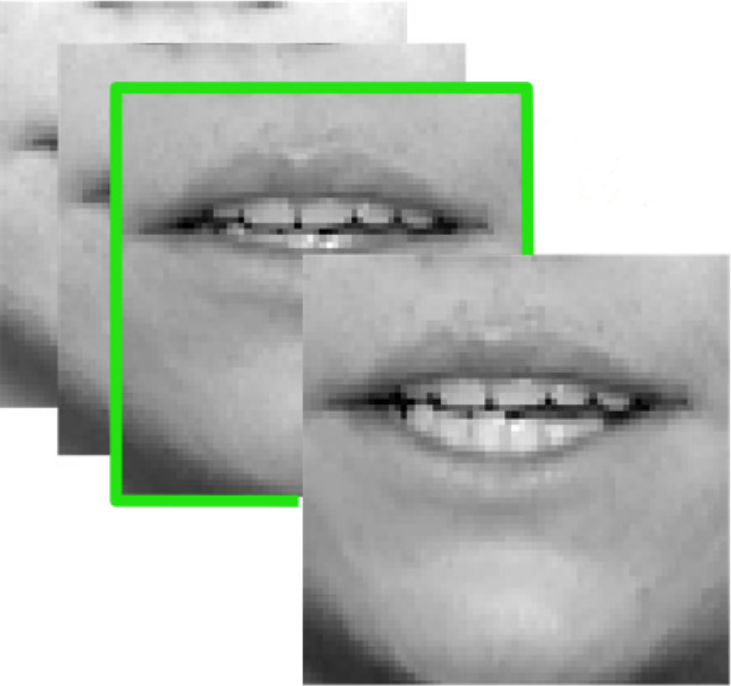
\includegraphics[width=.1\textwidth]{tikz/lips}};

  % mu, sigma, sample boxes
  \node [label={above:$\bs{\mu}^{av}_{\bs{\mylz}}(\bs{\myos}_n,\bs{\myov}_n)$}, fit=(mu-1) (mu-3), draw] (mu) {};
  \node [label={below:$\bs{\sigma}^{av}_{\bs{\mylz}}(\bs{\myos}_n,\bs{\myov}_n)$}, fit=(sigma-1) (sigma-3), draw] (sigma) {};
  \node [fit=(sample-1) (sample-3), draw] (sample) {};

  % mu, sigma, sample connections
  \draw[dashed] (mu.east) edge (sample.west) (sigma.east) -- (sample.west);
  \foreach \a in {1,2,3}
  \foreach \b in {1,2,3} {
      \draw[-] (encoder-2-\a) -- (mu-\b);
      \draw[-] (encoder-2-\a) -- (sigma-\b);
      \draw[-] (sample-\a) -- (decoder-1-\b);
      \draw[-] (cond-\a) -- (decoder-1-\b);
    }

  % input + output labels
%   \foreach \idx in {1,...,4} {
%       \node[left=0 of encoder-1-\idx] {$x_\idx$};
%       \node[right=0 of decoder-2-\idx] {$\hat x_\idx$};
%     }
  \node[above=0.1 of encoder-1-1] {$\bs{\myos}_n$};
  \node[below=0.1 of encoder-1-6] {$\bs{\myov}_n$};
  \node[above=0.1 of decoder-2-1] {$\hat{\bs{\myos}}_n$};

\end{tikzpicture}
}\vspace{2mm}
%   \includegraphics[width=\textwidth]{images/av_vae_new.pdf}
{\small
  $p_{\bs{\theta}}(\bs{\myos}_n | \bs{\mylz}_n,\bs{\myov}_n)= \mathcal{N}_c\Big(\boldsymbol{0}, \text{diag}(\bs{\sigma}_{\myos}(\bs{\mylz}_n,\bs{\myov}_n))\Big)$\vspace{3mm}\\
  $q_{\bs{\phi}}(\bs{\mylz}_n|\bs{\myov}_n,\bs{\myos}_n)= \mathcal{N}\Big(\bs{\mu}_{\bs{\mylz}}^{av}(\bs{\myov}_n,\bs{\myos}_n), \text{diag}(\bs{\sigma}_{\bs{\mylz}}^{av}(\bs{\myov}_n,\bs{\myos}_n))\Big)$}
 \end{column}
 \begin{column}{0.4\textwidth}
 \centering
 \only<2-3>{\alert{\Large What will this learn?}\vspace{2mm}\\}
 \only<3>{\Large To ignore the video!}
\only<4>{Visual Prior
 \resizebox{\textwidth}{!}{\input{tikz/v_prior_vae.tex}}
% \includegraphics[width=\textwidth]{images/prior_av_vae.pdf}
 {\small
  $p_{\bs{\theta}}(\bs{\mylz}_n|\bs{\myov}_n)= \mathcal{N}\Big(\bs{\mu}_{\bs{\mylz}}^v(\bs{\myov}_n), \text{diag}(\bs{\sigma}_{\bs{\mylz}}^v(\bs{\myov}_n))\Big)$}}
 \end{column}
\end{columns}
\end{frame}

%%%%%%%%%%%%%%%%%%%%%%%%%%%%%%%%%%%%%%%%%%%%%%%%%%%%%%%%%%%%%%%%%%%%%%%%%%%%
\begin{frame}{Learning AV Conditional VAE}
 On top of adding a video-only prior, we optimize a modified ELBO:
\begin{align*}
\hspace{-5mm}\mathcal{L}\left(\bs{\theta}, \bs{\phi} \right) =\sum_{n}  &{\alert{(1-\alpha)}}\Big(\E_{q_{\bs{\phi}}(\bs{z}_n|\bs{s}_n,\bs{v}_n;)}\Big[ \ln p_{\bs{\theta}}\left(\bs{s}_n | \bs{z}_n,\bs{v}_n \right) \Big]-D_{\text{KL}}\Big(q_{\bs{\phi}}\left(\bs{z}_n | \bs{s}_n,\bs{v}_n \right) \parallel p_{\bs{\theta}}(\bs{z}_n| \bs{v}_n)\Big)\Big)\\
\hspace{-5mm}& {+\alert{\alpha\,\E_{p_{\bs{\theta}}(\bs{z}_n| \bs{v}_n)}\Big[ \ln p_{\bs{\theta}}\left(\bs{s}_n | \bs{z}_n,\bs{v}_n \right) \Big]}}
\end{align*}

{$\Rightarrow \alpha>0 $ gives some reconstruction power to the visual prior!}

{This provides the parameters of the clean speech model $\bs{\theta}$. Let's enhance!}

\end{frame}


%%%%%%%%%%%%%%%%%%%%%%%%%%%%%%%%%%%%%%%%%%%%%%%%%%%%%%%%%%%%%%%%%%%%%%%%%%%
\begin{frame}{AV Conditional VAE for Speech Enhancement}
\begin{figure}
\centering
\only<1>{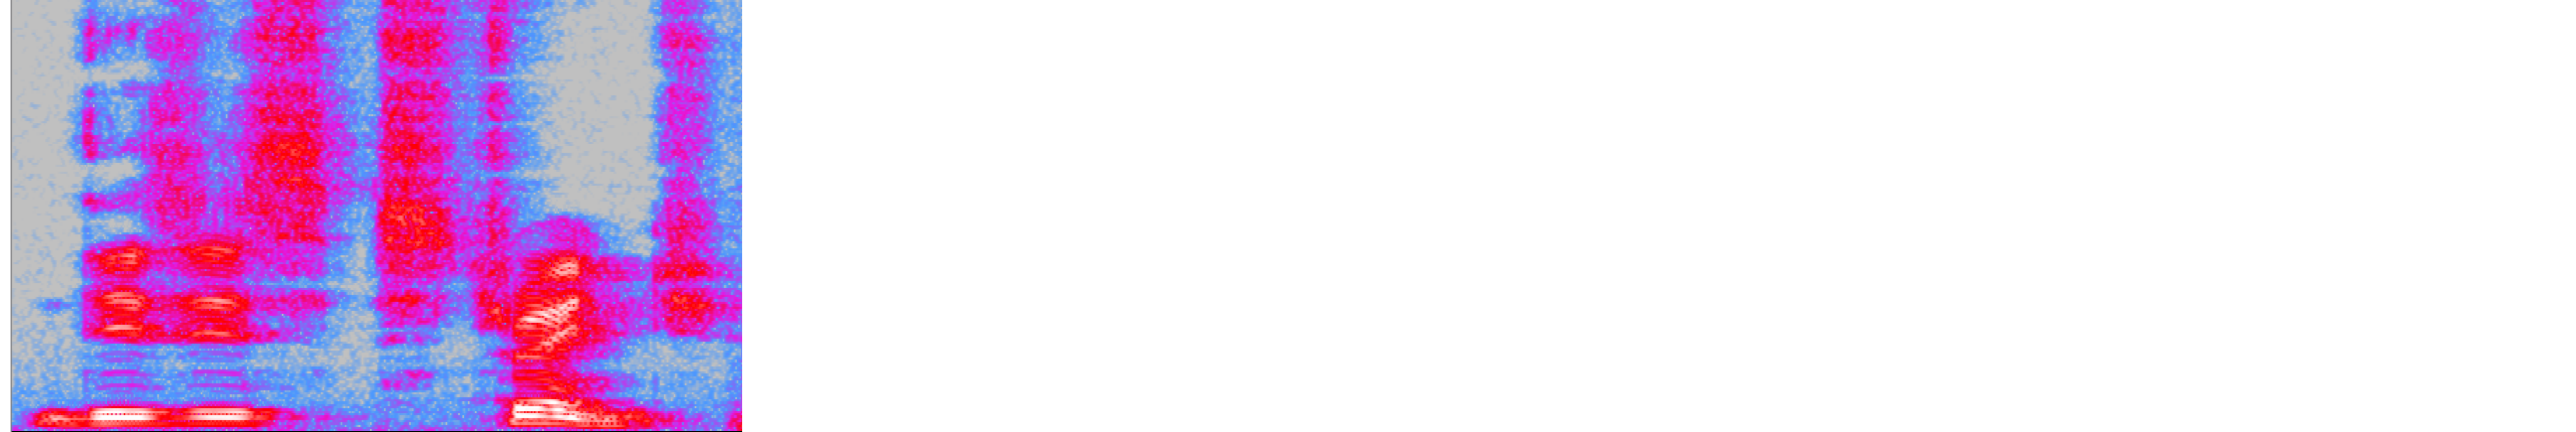
\includegraphics[width=0.8\textwidth]{images/spectrogram_cut.png}}%
\only<2->{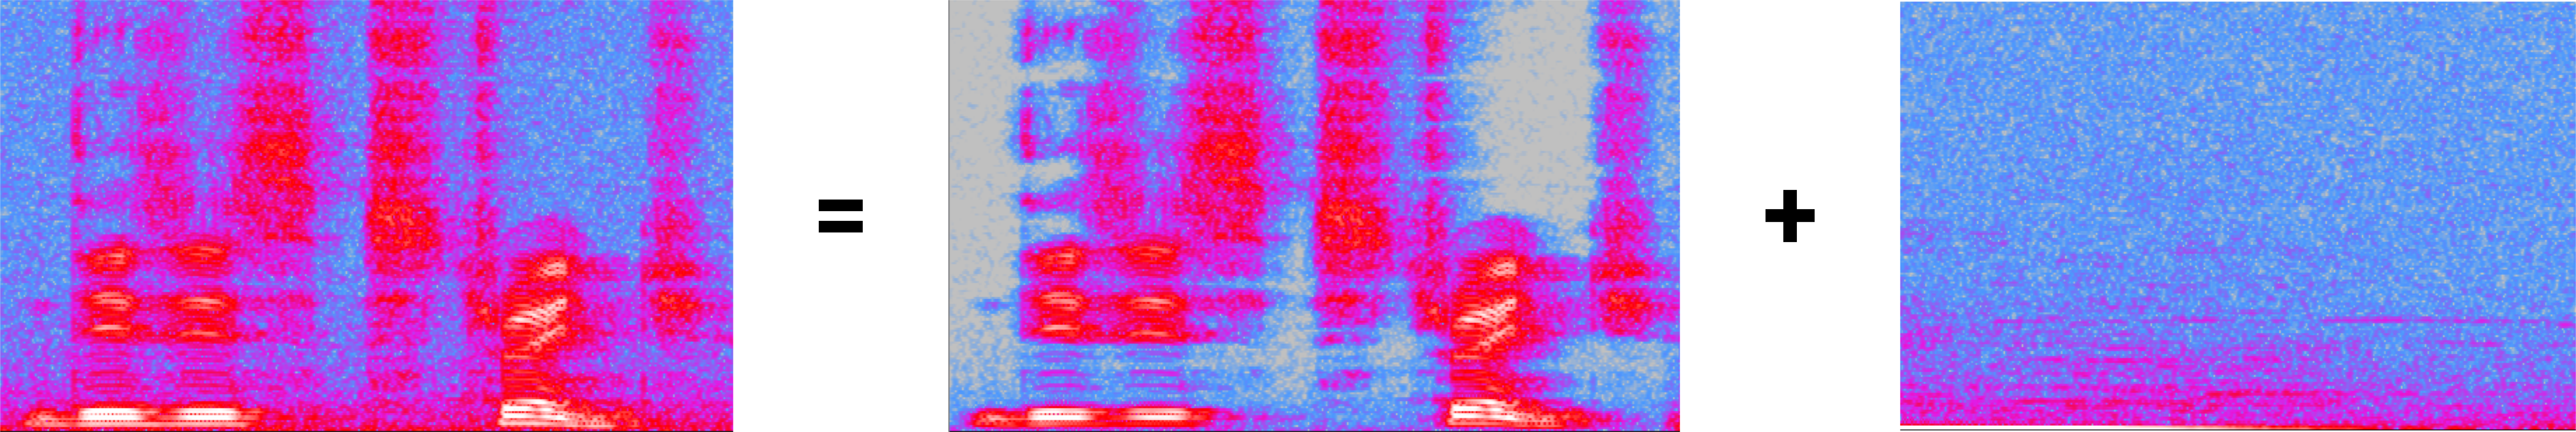
\includegraphics[width=0.8\textwidth]{images/spectrogram.png}}
\end{figure}
\vspace{-6mm}
\begin{equation*}
\only<1>{{\color{green}\underbrace{\mathbf{s}}_{\text{Clean speech}}} {\color{white}\quad\qquad+\quad\qquad \underbrace{\mathbf{b}}_{\text{Noise signal}}  \quad\qquad=\quad\qquad {\underbrace{\mathbf{x}}_{\text{Noisy mixture}}}}}
\only<2->{{\color{red}\underbrace{\mathbf{s}}_{\text{Clean speech}}} \quad\qquad+\quad\qquad {\color{gray}\underbrace{\mathbf{b}}_{\text{Noise signal}}}  \quad\qquad=\quad\qquad {\color{green}\underbrace{\mathbf{x}}_{\text{Noisy mixture}}}}
\end{equation*}

\begin{columns}
 \begin{column}{0.5\textwidth}
  \only<1>{\alert<1>{\textbf{Train}} -- Model for \textcolor<1>{green}{clean data}: $\{{\only<1>{\color{green}}\bs{s}_i}\}_{i=1}^N$.
    \begin{center}
    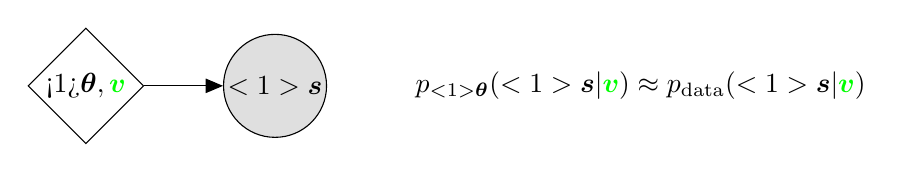
\begin{tikzpicture}
            \node[det] (theta) {\alert<1>{$\bs{\theta},\bs{\myov}$}};
            \node[obs,right=of theta] (s) {$\only<1>{\color{green}}\bs{s}$};
            \node[right=of s] (disc) {$p_{\alert<1>{\bs{\theta}}}({\only<1>{\color{green}}\bs{s}}|\bs{\myov})\approx p_{\text{data}}({\only<1>{\color{green}}\bs{s}}|\bs{\myov})$};
            \edge{theta} {s};
    \end{tikzpicture}
    \end{center}
    Then freeze $\alert<1>{\bs{\theta}}$ at test/adaptation time.}%
    \only<3>{\alert{\textbf{Speech Enhancement}}:\\
    {\small(Sample $\bs{\mylz}$ from $p(\bs{\mylz}|\bs{\myox}_n,\bs{\myov}_n)$)}
    \[\hat{\bs{\myls}}_{n} = \left(\frac{1}{R}\sum_{r=1}^R  \frac{ \bs{\sigma}_{\myls}(\mathbf{\mylz}^{(r)},\bs{\myov}_n)}{\bs{\sigma}_{\myls}(\mathbf{\mylz}^{(r)},\bs{\myov}_n) + \alert{\boldsymbol{\psi}}^\ast_n}\right) \bs{\myox}_{n}.\]
    Wiener-like filter!}
 \end{column}\pause
 \begin{column}{0.5\textwidth}
  \textbf{Test} -- learn the \alert{noise parameters} from {\color{green} noisy samples $\mathbf{x}$} and estimate the {\color{red} clean speech $\hat{\bs{s}}$}:
    \begin{center}
    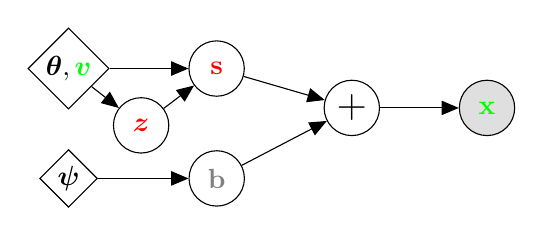
\begin{tikzpicture}
            \node[det] (theta) {$\bs{\theta},\bs{\myov}$};
            \only<3>{\node[latent,below right=of theta,xshift=-3mm,yshift=5mm] (z) {$\bs{\mylz}$};}
            \node[latent,right=of theta] (s) {$\color{red}\mathbf{s}$};
            \node[det,below=of theta,yshift=5mm] (eta) {$\alert{\bs{\psi}}$};
            \node[latent,right=of eta,xshift=1.5mm] (b) {$\color{gray}\mathbf{b}$};
            \node[latent,right=of s,yshift=-5mm] (plus) {\Large$+$};
            \node[obs,right=of plus] (x) {$\color{green}\mathbf{x}$};
            \edge{theta} {s};
            \edge{eta} {b};
            \edge{s,b} {plus};
            \edge{plus} {x};
            \only<3>{\edge{theta} {z}; \edge{z} {s};}
    \end{tikzpicture}
    \end{center}
 \end{column}
\end{columns}

% \textbf{Note}: at test time, $\bs{\theta}$ is frozen, and $\mathbf{s}$ becomes a latent variable.
\end{frame}

%%%%%%%%%%%%%%%%%%%%%%%%%%%%%%%%%%%%%%%%%%%%%%%%%%%%%%%%%%%%%%%%%%%%%%%%%%%%
\begin{frame}{But how do we learn $\bs{\psi}^*$?}
We opt for an EM-like solution. Given an initial value of the parameters $\bs{\psi}^0$:
\[Q(\alert{\bs{\psi}},\alert{\bs{\psi}}^0) = \sum_n\mathbb{E}_{p(\myls_n,\mylz_n|\myox_n,\myov_n;\alert{\bs{\psi}}^0,\bs{\theta})}[\log p(\myox_n,\myls_n,\mylz_n|\myov_n;\alert{\bs{\psi}},\bs{\theta})].\]\pause
Stop! There is an \textit{easier} way: $p(\myox_n,\mylz_n|\myov_n;\alert{\bs{\psi}})=\int p(\myox_n,\myls_n,\mylz_n|\myov_n;\alert{\bs{\psi}})\textrm{d}\myls_n $

Approximate $\mathcal{Q}$ via Monte-Carlo sampling:
\begin{itemize}
	\item \textbf{E-Step}: \hspace{.5cm} $ Q(\alert{\bs{\psi}}; \alert{\bs{\psi}}^0) \approx \sum_{n=1}^N \frac{1}{R} \sum_{r=1}^{R} \ln p(\myox_n, \mylz_n^{(r)} | \myov_n ; \alert{\bs{\psi}})$\\
{\small The samples $\left\{\mylz_n^{(r)}\right\}_{r=1,...,R}$ are i.i.d. and drawn from $p(\mylz_n | \myox_n, \myov_n ; \alert{\bs{\psi}}^0)$.}\vspace{3mm}
%
% \vspace*{0.5cm}
% $\triangleright$ {\small Note:~$ \ln p(\mathbf{x}, {\mathbf{z}^{(r)}}, \mathbf{v} ; \bs{\psi})= \ln p(\mathbf{x}| {\mathbf{z}^{(r)}}, \mathbf{v} ; \bs{\psi}) + \ln p({\mathbf{z}^{(r)}}| \mathbf{v})$}
%
%	\pause
% 	\vspace*{0.5cm}
	\item \textbf{M-Step}: \hspace{.5cm} $\alert{\bs{\psi}}^1 \leftarrow \argmax_{\alert{\bs{\psi}}} \, Q(\alert{\bs{\psi}}; \alert{\bs{\psi}}^0)\Rightarrow$  multiplicative update rules.\\
	{\small Standard formulae for NMF, not detailed here.}
\end{itemize}
\end{frame}

%%%%%%%%%%%%%%%%%%%%%%%%%%%%%%%%%%%%%%%%%%%%%%%%%%%%%%%%%%%%%%%%%%%%%%%%%%%%
\begin{frame}{Results}

{\small Performance measures (the higher, the better) -- improvement w.r.t.\ the noisy mixture:
	\begin{itemize}[]
		\item Perceptual evaluation of speech quality (PESQ).
		\item Signal-to-distortion ratio (SDR).
		\item Short-time objective intelligibility (STOI).
\end{itemize}}
\vspace*{-0.5cm}
{\small \begin{figure}[t]
		\centering
		\subfloat[{PESQ}]{{\includegraphics[width=3cm]{images/ALLAlgs_PESQ.pdf} }}\vspace{-1mm}
		\subfloat[{SDR}]{{\includegraphics[width=3cm]{images/ALLAlgs_SDR.pdf} }}\vspace{-1mm}
		\subfloat[{STOI}]{{\includegraphics[width=3cm]{images/ALLAlgs_STOI.pdf} }}
\end{figure}	}\vspace{3mm}


% {\footnotesize \textcolor{blue}{Audio Examples}: \url{https://team.inria.fr/perception/research/av-vae-se/}}

\end{frame}

%%%%%%%%%%%%%%%%%%%%%%%%%%%%%%%%%%%%%%%%%%%%%%%%%%%%%%%%%%%%%%%%%%%%%%%%%%%%
\begin{frame}{Limitations: systematic AV fusion}
 From the model design:\vspace{3mm}
 \begin{columns}
 \centering
  \begin{column}{0.6\textwidth}
    \resizebox{\textwidth}{!}{\renewcommand\drawNodes[2]{
  % #1 (str): namespace
  % #2 (list[list[str]]): list of labels to print in the node of each neuron
  \foreach \neurons [count=\lyrIdx] in #2 {
    \StrCount{\neurons}{,}[\lyrLength] % use xstring package to save each layer size into \lyrLength macro

    \ifthenelse{\equal{#1}{encoder}}{
        \ifnumequal{\lyrIdx}{1}
        {% True case
        \foreach \n [count=\nIdx] in \neurons
            \node[neuron,fill=green,fill opacity=0.2] (#1-\lyrIdx-\nIdx) at (0.7*\lyrIdx, \lyrLength/3.6-0.5*\nIdx) {\n};
        }
        {% False case
        \foreach \n [count=\nIdx] in \neurons
            \node[neuron] (#1-\lyrIdx-\nIdx) at (0.7*\lyrIdx, \lyrLength/3.6-0.5*\nIdx) {\n};
        }
    }{
        \ifnumequal{\lyrIdx}{2}
        {% True case
        \foreach \n [count=\nIdx] in \neurons
            \node[neuron,fill=green,fill opacity=0.2] (#1-\lyrIdx-\nIdx) at (0.7*\lyrIdx, \lyrLength/3.6-0.5*\nIdx) {\n};
        }
        {% False case
        \foreach \n [count=\nIdx] in \neurons
            \node[neuron] (#1-\lyrIdx-\nIdx) at (0.7*\lyrIdx, \lyrLength/3.6-0.5*\nIdx) {\n};
        }
    }
  }
}

\renewcommand\denselyConnectNodes[2]{
  % #1 (str): namespace
  % #2 (list[int]): number of nodes in each layer
  \foreach \n [count=\lyrIdx, remember=\lyrIdx as \previdx, remember=\n as \prevn] in #2 {
    \foreach \y in {1,...,\n} {
      \ifnum \lyrIdx > 1
        \foreach \x in {1,...,\prevn}
          \draw[-] (#1-\previdx-\x) -- (#1-\lyrIdx-\y);
      \fi
    }
  }
}

\begin{tikzpicture}[
    shorten >=1pt, shorten <=1pt,
    neuron/.style={circle, draw, minimum size=2ex, thick},
    legend/.style={font=\large\bfseries},
  ]

  % encoder
  \drawNodes{encoder}{{{,,,,,}, {,,}}}
  \denselyConnectNodes{encoder}{{6, 3}}

  % decoder
  \begin{scope}[xshift=3.7cm]
    \drawNodes{decoder}{{{,,}, {,,,}}}
    \denselyConnectNodes{decoder}{{3, 4}}
  \end{scope}
  
  \node[inner sep=0pt,left of=encoder-1-1,xshift=-0.5cm,yshift=-0.2cm] (input) {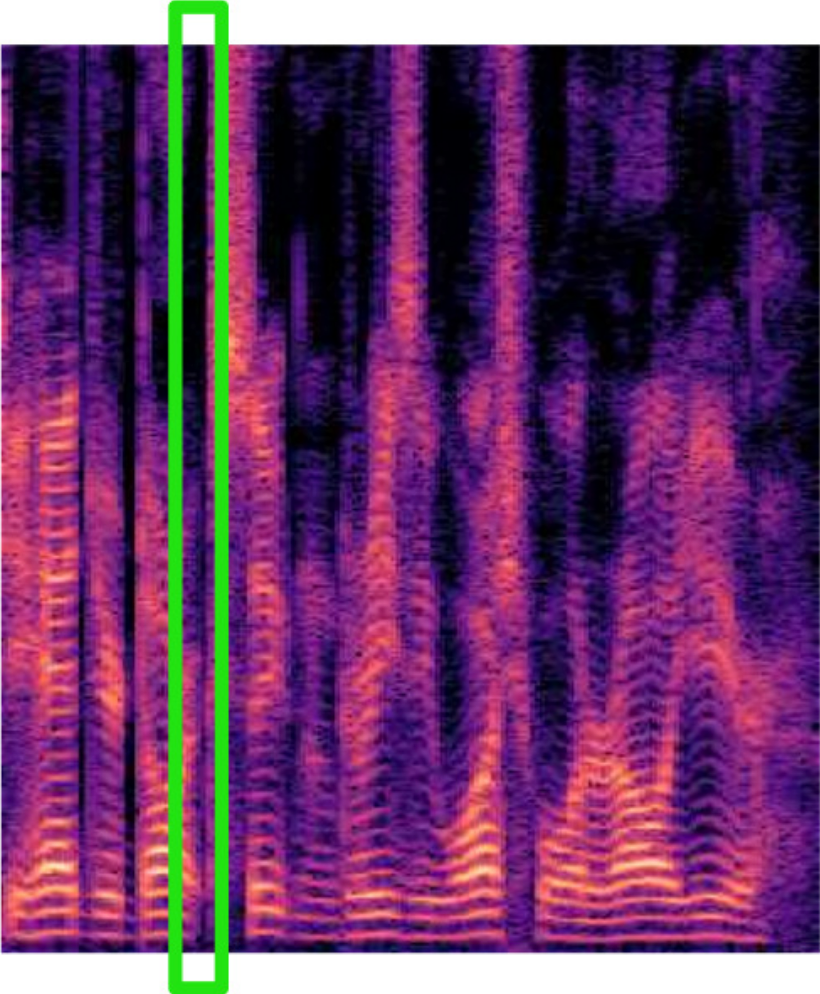
\includegraphics[width=.25\textwidth]{tikz/spectrogram}};
  \node[inner sep=0pt,left of=encoder-1-1,xshift=-0.5cm,yshift=-2.4cm] (input2) {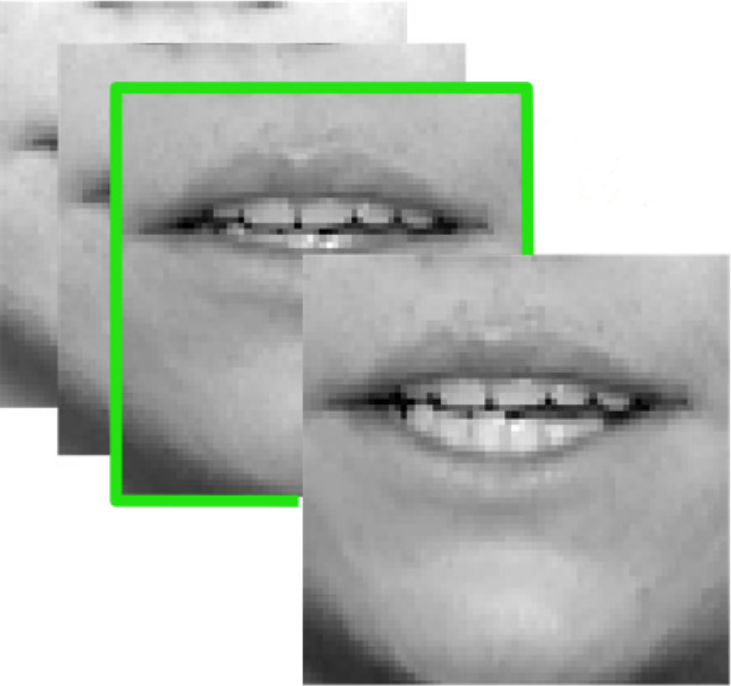
\includegraphics[width=.25\textwidth]{tikz/lips}};
  \node[inner sep=0pt,right of=decoder-2-1,xshift=0.5cm,yshift=-0.8cm] (output) {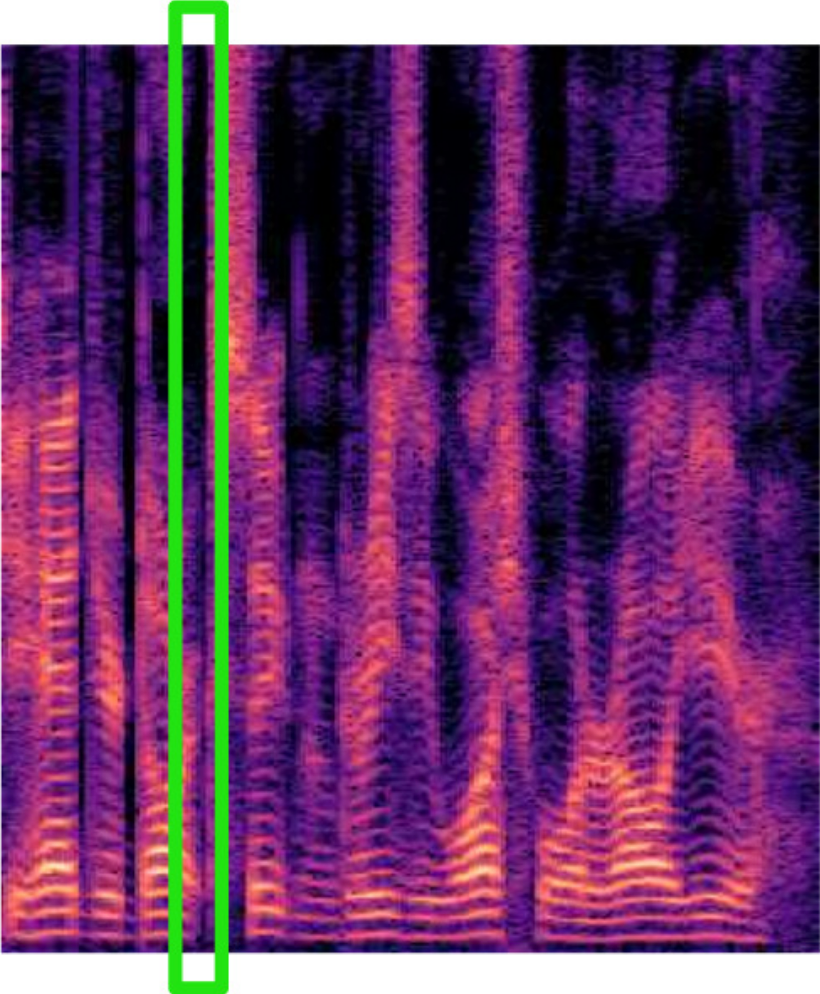
\includegraphics[width=.25\textwidth]{tikz/spectrogram}};
  
  % mu, sigma, sample nodes, conditioning
  \foreach \idx in {1,...,3} {
      \coordinate[neuron, right=2 of encoder-2-2, xshift=-1.4cm, yshift=0.5*\idx cm-0.15cm, fill=red, fill opacity=0.2] (mu-\idx);
      \coordinate[neuron, right=2 of encoder-2-2, xshift=-1.4cm, yshift=-0.5*\idx cm+0.15cm, fill=red, fill opacity=0.2] (sigma-\idx);
      \coordinate[neuron, right=4 of encoder-2-2, xshift=-2.2cm, yshift=0.5*\idx cm-.15cm, fill=red, fill opacity=0.2] (sample-\idx);
      \coordinate[neuron, right=4 of encoder-2-2, xshift=-2.2cm, yshift=0.5*\idx cm-1.85cm, fill=green, fill opacity=0.2] (cond-\idx);
    }
    
  \node[inner sep=0pt,below of=cond-1,xshift=0.2cm,yshift=0.2cm] (cond) {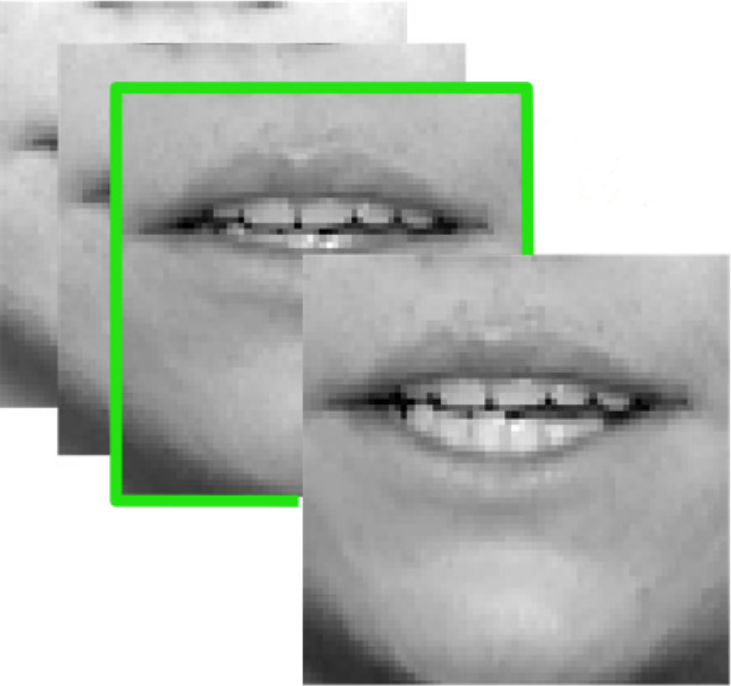
\includegraphics[width=.1\textwidth]{tikz/lips}};

  % mu, sigma, sample boxes
  \node [label={above:$\bs{\mu}^{av}_{\bs{\mylz}}(\bs{\myos}_n,\bs{\myov}_n)$}, fit=(mu-1) (mu-3), draw] (mu) {};
  \node [label={below:$\bs{\sigma}^{av}_{\bs{\mylz}}(\bs{\myos}_n,\bs{\myov}_n)$}, fit=(sigma-1) (sigma-3), draw] (sigma) {};
  \node [fit=(sample-1) (sample-3), draw] (sample) {};

  % mu, sigma, sample connections
  \draw[dashed] (mu.east) edge (sample.west) (sigma.east) -- (sample.west);
  \foreach \a in {1,2,3}
  \foreach \b in {1,2,3} {
      \draw[-] (encoder-2-\a) -- (mu-\b);
      \draw[-] (encoder-2-\a) -- (sigma-\b);
      \draw[-] (sample-\a) -- (decoder-1-\b);
      \draw[-] (cond-\a) -- (decoder-1-\b);
    }

  % input + output labels
%   \foreach \idx in {1,...,4} {
%       \node[left=0 of encoder-1-\idx] {$x_\idx$};
%       \node[right=0 of decoder-2-\idx] {$\hat x_\idx$};
%     }
  \node[above=0.1 of encoder-1-1] {$\bs{\myos}_n$};
  \node[below=0.1 of encoder-1-6] {$\bs{\myov}_n$};
  \node[above=0.1 of decoder-2-1] {$\hat{\bs{\myos}}_n$};

\end{tikzpicture}
}
  \end{column}
  \begin{column}{0.18\textwidth}
   \includegraphics<2->[width=\textwidth]{images/visual_clutter.png}
  \end{column}
 \end{columns}\vspace{3mm}
 . \only<2->{\alert{What about clutter?}}
\end{frame}


%%%%%%%%%%%%%%%%%%%%%%%%%%%%%%%%%%%%%%%%%%%%%%%%%%%%%%%%%%%%%%%%%%%%%%%%%%%%
\begin{frame}{VAE Mixture Model\footnote{Sadeghi, M., \textit{et. al.}, (2021), IEEE ICASSP.}}
  \begin{columns}
 \centering
  \begin{column}{0.6\textwidth}
    \resizebox{\textwidth}{!}{\renewcommand\drawNodes[2]{
  % #1 (str): namespace
  % #2 (list[list[str]]): list of labels to print in the node of each neuron
  \foreach \neurons [count=\lyrIdx] in #2 {
    \StrCount{\neurons}{,}[\lyrLength] % use xstring package to save each layer size into \lyrLength macro

    \ifthenelse{\equal{#1}{encoder}}{
        \ifnumequal{\lyrIdx}{1}
        {% True case
        \foreach \n [count=\nIdx] in \neurons
            \node[neuron,fill=green,fill opacity=0.2] (#1-\lyrIdx-\nIdx) at (0.7*\lyrIdx, \lyrLength/3.6-0.5*\nIdx) {\n};
        }
        {% False case
        \foreach \n [count=\nIdx] in \neurons
            \node[neuron] (#1-\lyrIdx-\nIdx) at (0.7*\lyrIdx, \lyrLength/3.6-0.5*\nIdx) {\n};
        }
    }{
        \ifnumequal{\lyrIdx}{2}
        {% True case
        \foreach \n [count=\nIdx] in \neurons
            \node[neuron,fill=green,fill opacity=0.2] (#1-\lyrIdx-\nIdx) at (0.7*\lyrIdx, \lyrLength/3.6-0.5*\nIdx) {\n};
        }
        {% False case
        \foreach \n [count=\nIdx] in \neurons
            \node[neuron] (#1-\lyrIdx-\nIdx) at (0.7*\lyrIdx, \lyrLength/3.6-0.5*\nIdx) {\n};
        }
    }
  }
}

\renewcommand\denselyConnectNodes[2]{
  % #1 (str): namespace
  % #2 (list[int]): number of nodes in each layer
  \foreach \n [count=\lyrIdx, remember=\lyrIdx as \previdx, remember=\n as \prevn] in #2 {
    \foreach \y in {1,...,\n} {
      \ifnum \lyrIdx > 1
        \foreach \x in {1,...,\prevn}
          \draw[-] (#1-\previdx-\x) -- (#1-\lyrIdx-\y);
      \fi
    }
  }
}

\begin{tikzpicture}[
    shorten >=1pt, shorten <=1pt,
    neuron/.style={circle, draw, minimum size=2ex, thick},
    legend/.style={font=\large\bfseries},
  ]

  % decoder-a
  \drawNodes{decoder-a}{{{,,}, {,,,}}}
  \denselyConnectNodes{decoder-a}{{3, 4}}

  % decoder-av
  \begin{scope}[yshift=-3.5cm]
    \drawNodes{decoder-av}{{{,,}, {,,,}}}
    \denselyConnectNodes{decoder-av}{{3, 4}}
  \end{scope}
  
%   \node[inner sep=0pt,left of=encoder-1-1,xshift=-0.5cm,yshift=-0.2cm] (input) {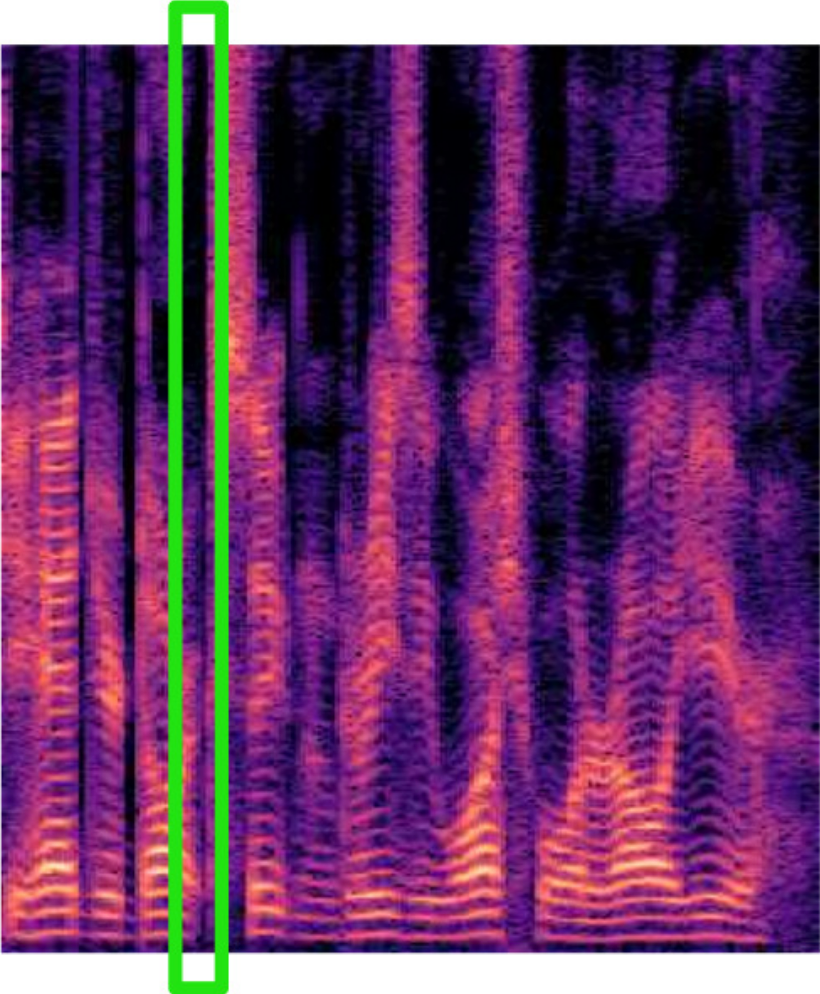
\includegraphics[width=.25\textwidth]{tikz/spectrogram}};
%   \node[inner sep=0pt,left of=encoder-1-1,xshift=-0.5cm,yshift=-2.4cm] (input2) {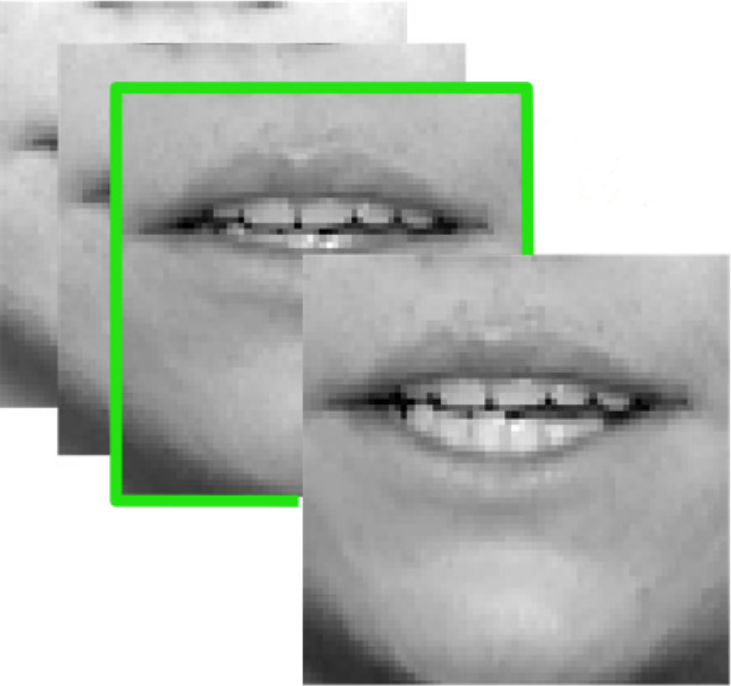
\includegraphics[width=.25\textwidth]{tikz/lips}};
  
  % mu, sigma, sample nodes, conditioning
  \foreach \idx in {1,...,3} {
%       \coordinate[neuron, right=2 of encoder-2-2, xshift=-1.4cm, yshift=0.5*\idx cm-0.15cm, fill=red, fill opacity=0.2] (mu-\idx);
%       \coordinate[neuron, right=2 of encoder-2-2, xshift=-1.4cm, yshift=-0.5*\idx cm+0.15cm, fill=red, fill opacity=0.2] (sigma-\idx);
      \coordinate[neuron, left=of decoder-a-1-\idx, xshift=6mm, fill=red, fill opacity=0.2] (sample-a-\idx);
      \coordinate[neuron, left=of decoder-av-1-1, xshift=6mm, yshift=0.5*\idx cm-0.4cm, fill=red, fill opacity=0.2] (sample-av-\idx);
      \coordinate[neuron, left=of decoder-av-1-1, xshift=6mm,yshift=0.5*\idx cm-2.3cm, fill=green, fill opacity=0.2] (cond-av-\idx);
    }
    
  \node[left=of sample-a-1,xshift=6mm,yshift=-2mm] (post-a) {\textcolor{blue}{Audio-only VAE}};
  \node[below=of post-a,yshift=1cm] {$q^a_{\bs{\phi}}(\bs{\mylz}_n|\bs{\myos}_n,\bs{\myov}_n)$};
  
  \node[left=of sample-av-3,xshift=6mm,yshift=-2mm] (post-av) {\textcolor{magenta}{Audio-Visual VAE}};
  \node[below=of post-av,yshift=1cm] {$q^{av}_{\bs{\phi}}(\bs{\mylz}_n|\bs{\myos}_n,\bs{\myov}_n)$};  
    
  \node[inner sep=0pt,left of=cond-av-1,xshift=-.5cm,yshift=5mm] (cond) {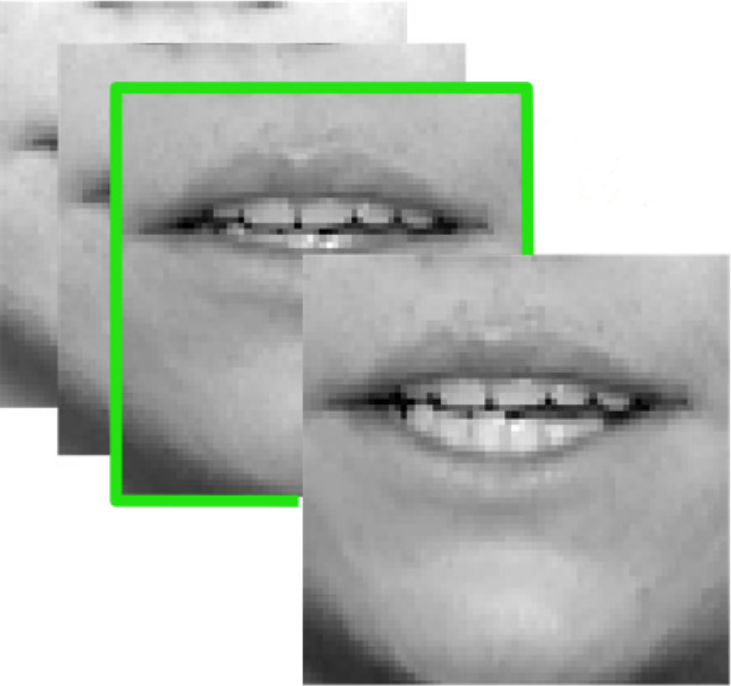
\includegraphics[width=.15\textwidth]{tikz/lips}};

  % mu, sigma, sample boxes
%   \node [label={above:$\bs{\mu}^{av}_{\bs{\mylz}}(\bs{\myos}_n,\bs{\myov}_n)$}, fit=(mu-1) (mu-3), draw] (mu) {};
%   \node [label={below:$\bs{\sigma}^{av}_{\bs{\mylz}}(\bs{\myos}_n,\bs{\myov}_n)$}, fit=(sigma-1) (sigma-3), draw] (sigma) {};
%   \node [fit=(sample-av-1) (sample-av-3), draw] (sample-av) {};
%   \node [fit=(sample-a-1) (sample-a-3), draw] (sample-a) {};

  \node [fit=(decoder-a-2-1) (decoder-a-2-4), draw] (decoder-a-2) {};
  \node [fit=(decoder-av-2-1) (decoder-av-2-4), draw] (decoder-av-2) {};
  \node [fit=(post-av) (sample-av-3) (cond-av-1) (decoder-av-2), draw=magenta, very thick] (vae-av) {};
  \node [fit=(post-a) (decoder-a-2), draw=blue, very thick] (vae-a) {};
  
  \node[circle,draw,below right=of decoder-a-2,yshift=9mm] (alpha) {$\bs{\alpha}_n$};
  \draw[->,blue] (vae-a.east) -- node[above,xshift=8mm] {$p_{\bs{\theta}}(\bs{\myos}_n|\bs{\mylz}^{a}_n)$} ++ (alpha);
  \draw[->,magenta] (vae-av.east) -- node[below,xshift=10mm] {$p_{\bs{\theta}}(\bs{\myos}_n|\bs{\mylz}^{av}_n,\bs{\myov}_n)$} ++ (alpha);
  % mu, sigma, sample connections
%   \draw[dashed] (mu.east) edge (sample.west) (sigma.east) -- (sample.west);
  \foreach \a in {1,2,3}
  \foreach \b in {1,2,3} {
%       \draw[-] (encoder-2-\a) -- (mu-\b);
      \draw[-] (sample-a-\a) -- (decoder-a-1-\b);
      \draw[-] (sample-av-\a) -- (decoder-av-1-\b);
      \draw[-] (cond-av-\a) -- (decoder-av-1-\b);
    }

    \node[inner sep=0pt,right of=alpha,xshift=1.5cm] (output) {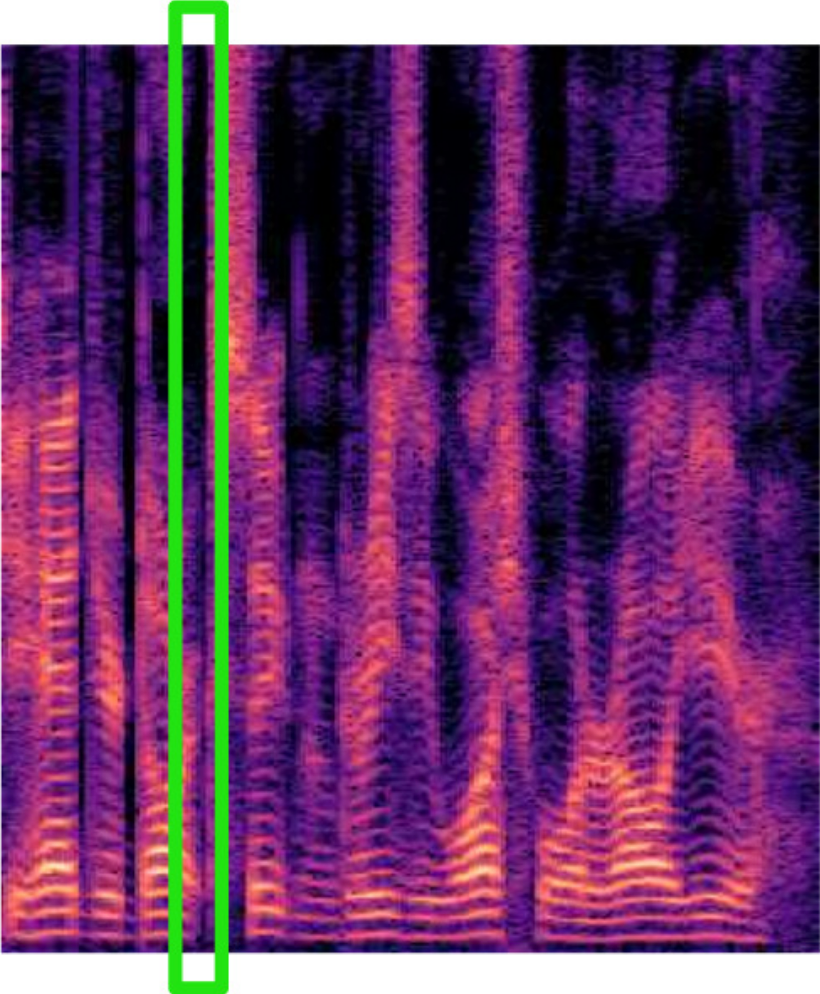
\includegraphics[width=.25\textwidth]{tikz/spectrogram}};
    \draw[->] (alpha) -- (output);
    
  % input + output labels
%   \foreach \idx in {1,...,4} {
%       \node[left=0 of encoder-1-\idx] {$x_\idx$};
%       \node[right=0 of decoder-2-\idx] {$\hat x_\idx$};
%     }
%   \node[above=0.1 of encoder-1-1] {$\bs{\myos}_n$};
%   \node[below=0.1 of encoder-1-6] {$\bs{\myov}_n$};
%   \node[above=0.1 of decoder-a-2-1] {$\hat{\bs{\myos}}_n$};
%   \node[below=0.1 of decoder-av-2-4] {$\hat{\bs{\myos}}_n$};

\end{tikzpicture}
}
  \end{column}
  \begin{column}{0.4\textwidth}
    $\bs{\alpha}_n$ is the ``mixing'' latent variable.\vspace{-2mm}
    \[\begin{cases}
       \bs{\alpha}_n=1 \leftrightarrow \text{\color{blue}Audio-only}\\
       \bs{\alpha}_n=0 \leftrightarrow \text{\color{magenta}Audio-Visual}
      \end{cases}\vspace{-2mm}
    \]
    Prior: $p(\alpha_n) = \textcolor{blue}{\pi}^{\alpha_n} (\textcolor{magenta}{1-\pi})^{1-\alpha_n}.$\vspace{8mm}\\
    The \textcolor{blue}{Audio-only} and the \textcolor{magenta}{Audio-Visual} VAE are \textbf{\alert{mixed without supervision}}.
  \end{column}
 \end{columns}
\end{frame}

%%%%%%%%%%%%%%%%%%%%%%%%%%%%%%%%%%%%%%%%%%%%%%%%%%%%%%%%%%%%%%%%%%%%%%%%%%%%
\begin{frame}{Train, adaptation \& speech enhancement}
\begin{columns}
\begin{column}{0.35\textwidth}
\begin{center}
\begin{tikzpicture}
% Audio-only (blue)
\node[det,draw=blue] (theta-a) {${\color{blue}\bs{\theta}^{a}}$};
\node[latent,below right=of theta-a,xshift=-1.5mm,yshift=5mm,draw=blue] (z-a) {$\bs{\mylz}^{\color{blue}a}$};
\node[latent,right=of theta-a,draw=blue,xshift=3mm] (s-a) {$\bs{\only<1>{\myos}\only<2->{\myls}}^{\color{blue}a}$};
\node[fit=(theta-a) (s-a) (z-a),draw=blue] (a-vae) {};
\edge[draw=blue]{theta-a} {s-a};
\edge[draw=blue] {theta-a} {z-a}; \edge[draw=blue]{z-a} {s-a};
% Audio-visual (magenta)
\node[det,below=of theta-a,draw=magenta,yshift=-1mm] (theta-av) {${\color{magenta}\bs{\theta}^{av}},\bs{\myov}$};
\node[latent,below right=of theta-av,xshift=-3mm,yshift=5mm,draw=magenta] (z-av) {$\bs{\mylz}^{\color{magenta}av}$};
\node[latent,right=of theta-av,draw=magenta] (s-av) {$\bs{\only<1>{\myos}\only<2->{\myls}}^{\color{magenta}av}$};
\node[fit=(theta-av) (s-av) (z-av),draw=magenta] (av-vae) {};
\edge[draw=magenta]{theta-av} {s-av};
\edge[draw=magenta] {theta-av} {z-av}; \edge[draw=magenta]{z-av} {s-av};
% Mixing variable
\only<2->{\node[latent,below right=of s-a,yshift=2mm] (s) {$\myls$};
\node[latent,above=of s,yshift=2mm] (alpha) {$\bs{\color{red}\alpha}$};
\edge[->]{s-a,s-av,alpha} {s};}
% Noise
\only<3->{\node[det,below=of theta-av] (eta) {$\alert{\bs{\psi}}$};
\node[latent,right=of eta,xshift=3mm] (b) {$\color{gray}\mathbf{b}$};
\node[fit=(eta) (b),draw] (a-vae) {};
\edge{eta} {b};}
% Combining
\only<4->{\node[latent,below=of s] (plus) {\Large$+$};
\node[obs,below=of plus] (x) {$\color{green}\mathbf{x}$};
\edge{s,b} {plus};
\edge{plus} {x};}

\end{tikzpicture}
\end{center}
\end{column}%
\begin{column}{0.7\textwidth}
 \begin{itemize}
  \item Train \textcolor{blue}{A-VAE} (with $\bs{\myos}$) and \textcolor{magenta}{AV-VAE} (with $(\bs{\myos},\bs{\myov})$).
  \item<2-> The clean speeh is now \textcolor{red}{latent} ($\bs{\myls}^{\color{blue}a}, \bs{\myls}^{\color{magenta}av}$), add the\\ \textcolor{red}{mixing latent} variable ($\bs{\color{red}\alpha}$).
  \item<3-> We also consider the noise variable and params.
  \item<4-> Learn $\alert{\bs{\psi}}^\ast$ and estimate the clean speech. \only<4->{By defining\\
  {\small$\bs{\gamma}_{n}(\bs{\mylz}_n,\bs{\myov}_n) = \left( {\color{blue}\pi_n} ({\color{blue}\bs{\sigma}^a_{s}(\bs{\mylz}_n)})^{-1} + ({\color{magenta}1-\pi_n})({\color{magenta}\bs{\sigma}^{av}_{s}(\bs{\mylz}_n,\bs{\myov}_n)})^{-1}\right)^{-1}$}}\only<5->{:
  \begin{align*}
\label{source_estimate}
\hat{\bs{s}}_{n}
&= \frac{1}{R}\sum_{r=1}^R  \frac{ \bs{\gamma}_{n}(\bs{\mylz}_n^{(r)},\bs{\myov}_n)}{
	\bs{\gamma}_{n}(\bs{\mylz}_n^{(r)},\bs{\myov}_n) + \bs{\alert{\psi}}^\ast_n}\,\bs{\myox}_{n}
\end{align*}}
 \end{itemize}
\end{column}
\end{columns}
\end{frame}

\begin{frame}{Learning the noise parameters with VAE-MM}
 \textbf{Ideally}:
\[Q(\bs{\psi},\bs{\psi}^0) = \sum_{n=1}^N\E_{\alert{p(\bs{s}_n, \bs{z}_n, \alpha_n|\mathbf{x}_n,\bs{v}_n;\bs{\psi}^0)}} [\log p(\mathbf{x}_n,\bs{s}_n, \bs{z}_n, \alpha_n|\bs{v}_n;\bs{\psi})]\]
We need to approximate this posterior:
\[p(\bs{s}_n, \bs{z}_n, \alpha_n|\mathbf{x}_n,\bs{v}_n;\bs{\psi}^0) \approx q(\bs{s}_n, \bs{z}_n, \alpha_n) = q_{\bs{s}}(\bs{s}_n)\; q_{\bs{z}}(\bs{z}_n)\; q_{\alpha}(\alpha_n).\]
Of course we will need to sample from $q_{\bs{z}}$, but in that case:
\begin{enumerate}
 \item $q_{\alpha}$ is a Bernoulli distribution.
 \item $q_{\bs{s}}$ is a complex Gaussian distribution.
\end{enumerate}

\end{frame}

%%%%%%%%%%%%%%%%%%%%%%%%%%%%%%%%%%%%%%%%%%%%%%%%%%%%%%%%%%%%%%%%%%%%%%%%%%%%
\begin{frame}{Settings \& Results}

\begin{itemize}
\item \textbf{Noisy+clean speech}: NTCD-TIMIT database {\footnotesize [Abdelaziz, 2017]}
\item \textbf{VAE models}: Pre-trained A-VAE and AV-VAE {\footnotesize [Sadeghi et al., 2019]}
\item \textbf{Setup}: Very similar than in the previous experiments. \alert{Clean and noisy} lips region visual information ($\sim$ one-third of total video frames per sample).
\end{itemize}

Improvement with respect to the input:\vspace{-3mm}
\setcounter{subfigure}{0}% Reset subfigure counter
\begin{figure}[t]
\centering
{\small\subfloat[{PESQ \textcolor{green}{(clean)}}]{{\includegraphics[height=2.9cm]{images/New3_mix_a_av_PESQ.pdf} }}\vspace{-2mm}
\subfloat[{SDR \textcolor{green}{(clean)}}]{{\includegraphics[height=2.9cm]{images/New3_mix_a_av_SDR.pdf} }}
\subfloat[{PESQ \textcolor{red}{(noisy)}}]{{\includegraphics[height=2.9cm]{images/randOCC20_New3_mix_a_av_PESQ.pdf} }}
\subfloat[{SDR \textcolor{red}{(noisy)}}]{{\includegraphics[height=2.9cm]{images/randOCC20_New3_mix_a_av_SDR.pdf} }}}
\vspace{-2.5mm}
\end{figure}

\end{frame}


%%%%%%%%%%%%%%%%%%%%%%%%%%%%%%%%%%%%%%%%%%%%%%%%%%%%%%%%%%%%%%%%%%%%%%%%%%%%
\begin{frame}{Conditional VAE, VAE-MM and Mixture of Inference Networks VAE}
\vspace{-3mm}
\begin{columns}
  \begin{column}{0.5\textwidth}
   \centering\includegraphics[width=.9\textwidth]{images/av_vae_new.pdf}
  \end{column}
  \begin{column}{0.5\textwidth}\small
   Conditional VAE:\vspace{-2mm}
   \begin{itemize}
    \item Training VAE via SGD.\vspace{-2mm}
    \item Systematic AV fusion.\vspace{-2mm}
    \item Enhancement via MECM.
%     \item Appeared at IEEE TASLP in 2020.
   \end{itemize}
  \end{column}
 \end{columns}\vspace{1mm}\hrule\vspace{1mm}
 \begin{columns}
  \begin{column}{0.5\textwidth}
   \centering\includegraphics[width=.5\textwidth]{images/mix_a_av.pdf}
  \end{column}
  \begin{column}{0.5\textwidth}\small
   VAE-MM:\vspace{-2mm}
   \begin{itemize}
    \item Training two VAEs via SGD.\vspace{-2mm}
    \item Mixing (AV fusion) via two speech models.\vspace{-2mm}
    \item Enhancement via VEM + sampling.
%     \item Appeared at IEEE ICASSP in 2021.
   \end{itemize}
  \end{column}
 \end{columns}\vspace{1mm}\hrule\vspace{1mm}
 \begin{columns}
  \begin{column}{0.5\textwidth}
   \centering\includegraphics[width=.9\textwidth]{images/mix_ave.pdf}
  \end{column}
  \begin{column}{0.5\textwidth}\small
   MIN-VAE:\vspace{-2mm}
   \begin{itemize}
    \item Training all 3 networks via VEM+SGD.\vspace{-2mm}
    \item Mixing (AV fusion) via a single speech model.\vspace{-2mm}
    \item Enhancement via VEM + sampling.
%     \item Appeared at IEEE TSP in 2021.
   \end{itemize}
  \end{column}
 \end{columns}\vspace{-8mm}
\end{frame}

%%%%%%%%%%%%%%%%%%%%%%%%%%%%%%%%%%%%%%%%%%%%%%%%%%%%%%%%%%%%%%%%%%%%%%%%%%%%
\begin{frame}{Strong limitation of VAEs: frame modeled independently.}
\begin{center}
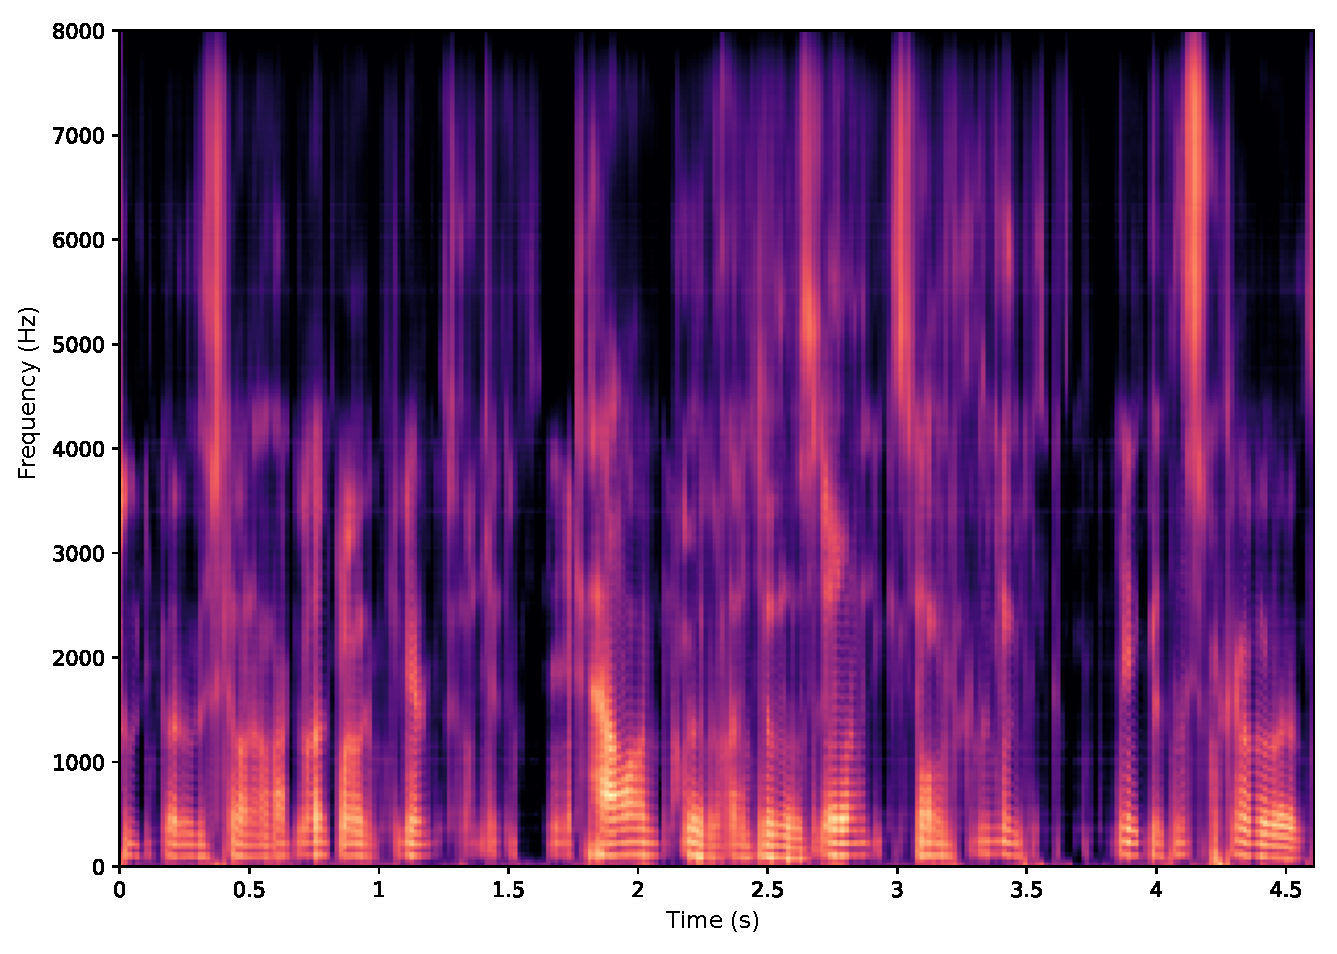
\includegraphics[height=0.3\textwidth]{images/generated_SRNN.pdf}\hspace{2mm}
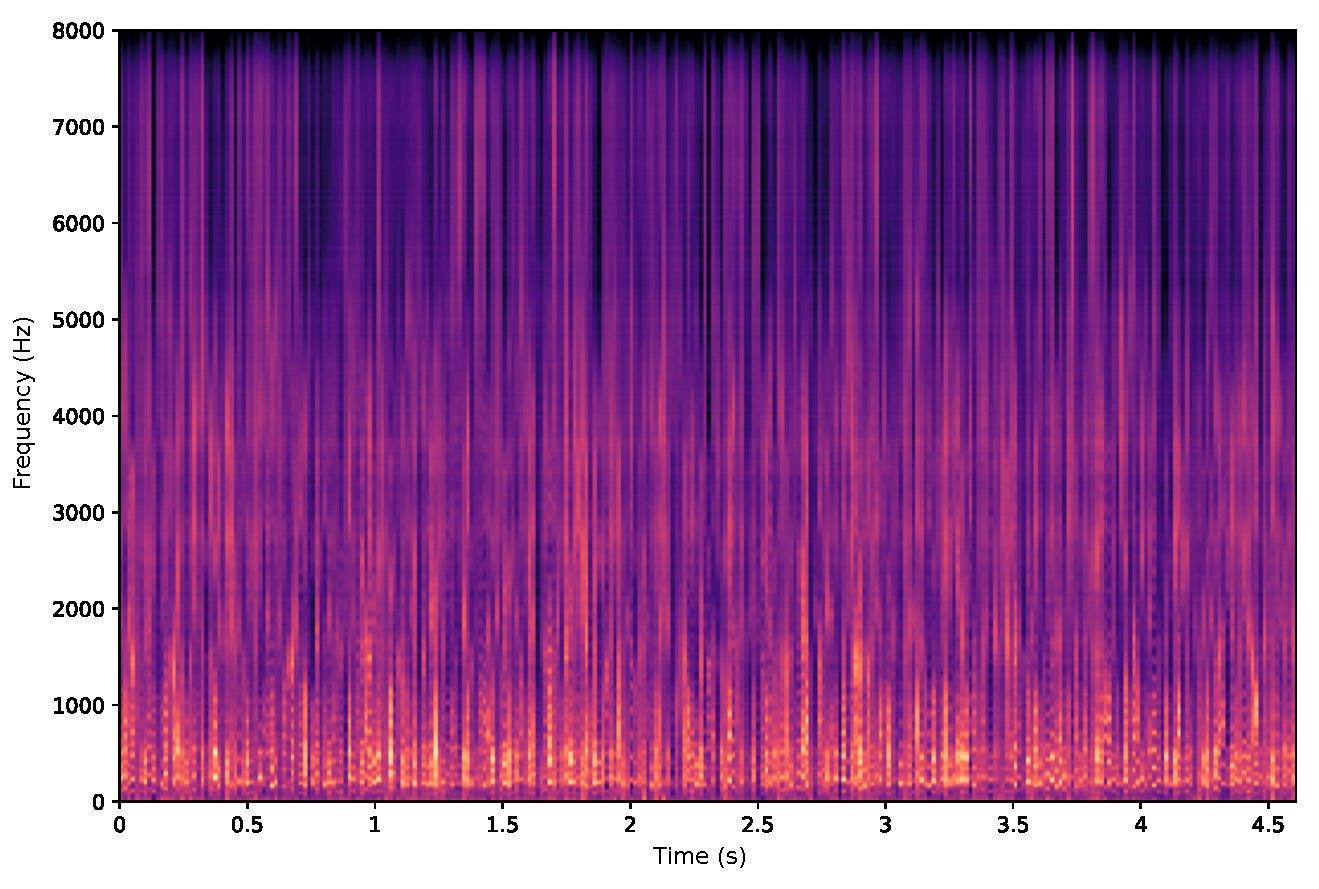
\includegraphics[height=0.3\textwidth]{images/generated_VAE.pdf}\\
Frames are modeled independently, we need time/sequential modeling!
\end{center}
\end{frame}

{\setbeamercolor{background canvas}{bg=mDarkTeal}
\setbeamercolor{background canvas}{fg=white}
\begin{frame}%{Restricted to RNN?}
  \color{white}\large\bf
  $\blacktriangleright$ \alert{Dynamical} VAE (\alert{\bf DVAE}\footnote{\color{white}Girin, L., \textit{et. al.}, (2021), FnT Machine Learning -- \texttt{Warning $\sim$ 150 pages}!!}) -- ``VAE for sequential modeling''\vspace{3mm}\\ (family of methods including existing literature)
  \vspace{1cm}
\begin{columns}
 \begin{column}{3cm}
    \centering
    \includegraphics[width=.66\textwidth]{people/xiaoyu.png}\\
    \color{white}Xiaoyu Bie
 \end{column}
 \begin{column}{3cm}
    \centering
    \includegraphics[width=.66\textwidth]{people/laurent.png}\\
    \color{white}Laurent Girin
 \end{column}
 \begin{column}{3cm}
    \centering
    \includegraphics[width=.66\textwidth]{people/simon.png}\\
    \color{white}Simon Leglaive
 \end{column}
  \begin{column}{3.4cm}
    \centering
    \includegraphics[width=.6\textwidth]{people/thomas.png}\\
    \color{white}Thomas Hueber
 \end{column}
 \begin{column}{3cm}
    \centering
    \includegraphics[width=.66\textwidth]{people/julien.png}\\
    \color{white}Julien Diard
 \end{column}
\end{columns}
\end{frame}
}


%%%%%%%%%%%%%%%%%%%%%%%%%%%%%%%%%%%%%%%%%%%%%%%%%%%%%%%%%%%%%%%%%%%%%%%%%%%%
\begin{frame}{Probabilistic Sequential Modeling (decoder network)}
We would like to model sequences of observations ($\bs{x}_{1:T}$) and latent variables ($\bs{z}_{1:T})$:
\[p^{\textrm{DVAE}}_{\bs{\theta}}(\bs{x}_{1:T}, \bs{z}_{1:T}) \alert{\neq}  \prod_{t=1}^T p_{\bs{\theta}}(\bs{x}_t,\bs{z}_t) = p^{\textrm{VAE}}_{\bs{\theta}}(\bs{x}_{1:T}, \bs{z}_{1:T}).\]
\vspace{-10mm}
\begin{columns}
 \begin{column}{0.3\textwidth}
 $ $\vspace{15mm}\\
  \foreach \index in {1, ..., 7}
{%
  \only<\index>{\includegraphics[width=\textwidth]{images/BN_\index.png}}\par%
}%
 \end{column}
 \begin{column}{0.7\textwidth}
\only<7>{\[ p_{\bs{\theta}}(\bs{x}_{1:T}, \bs{z}_{1:T} ) = \prod_{t=1}^T  p_{\bs{\theta}}(\bs{z}_t | \bs{x}_{1:t-1}, \bs{z}_{1:t-1} ) p_{\bs{\theta}}(\bs{x}_t | \bs{x}_{1:t-1}, \bs{z}_{1:t} )\]
 The \textit{prior} distribution $p_{\bs{\theta}}(\bs{z}_{t+1}|\bs{z}_{1:t},\bs{x}_{1:t})$ is now conditional, parametric, and might be auto-regressive (AR).\vspace{3mm}\\

  $p_{\bs{\theta}}(\bs{x}_{t+1}|\bs{z}_{1:t+1},\bs{x}_{1:t})$ might be AR as well.}
 \end{column}
\end{columns}
\end{frame}

%%%%%%%%%%%%%%%%%%%%%%%%%%%%%%%%%%%%%%%%%%%%%%%%%%%%%%%%%%%%%%%%%%%%%%%%%%%%
\begin{frame}{Probabilistic Sequential Inference (encoder network)}
 As in the VAE, we need to approximate the posterior distribution:
 \[ p_{\bs{\theta}}(\bs{z}_{1:T}|\bs{x}_{1:T}) = q_{\bs{\phi}}(\bs{z}_{1:T}|\bs{x}_{1:T})\]\pause
 We can always use the Bayes theorem to write:
 \[q_{\bs{\phi}}(\bs{z}_{1:T}|\bs{x}_{1:T}) = \prod_{t=1}^T q_{\bs{\phi}}(\bs{z}_{t}|\bs{z}_{1:t-1},\bs{x}_{1:T})\]
 Can we simplify each of the terms further? It depends on generative model. Use \alert{D-separation}\footnote{Bishop, C. M., (2006).} to find out the true dependencies, then choose whether to keep them (e.g.\ to ensure causality).
\end{frame}

%%%%%%%%%%%%%%%%%%%%%%%%%%%%%%%%%%%%%%%%%%%%%%%%%%%%%%%%%%%%%%%%%%%%%%%%%%%%
\begin{frame}{Implementation (both decoder and encoder)}

Let's take the general DVAE decoder:
$$ p_{\bs{\theta}}({\color{green}\bs{x}_{1:T}}, {\color{red}\bs{z}_{1:T}} ) =  \prod_{t=1}^T  p_{\bs{\theta}_{\color{red}\bs{z}}}({\color{red}\bs{z}_t} | {\color{green}\bs{x}_{1:t-1}}, {\color{red}\bs{z}_{1:t-1}} ) p_{\bs{\theta}_{\color{green}\bs{x}}}({\color{green}\bs{x}_t} | {\color{green}\bs{x}_{1:t-1}}, {\color{red}\bs{z}_{1:t}} ).$$\vspace{-4mm}\pause

The generative distributions can be implemented with an RNN:

- ${\color{magenta}\bs{h}_{t}} = \sigma(\bs{W}_{xh} {\color{green}\bs{x}_{t-1}} + \bs{W}_{zh} {\color{red}\bs{z}_{t-1}}  + \bs{W}_{hh} {\color{magenta}\bs{h}_{t-1}} + \bs{b}_h),$

- $p_{\bs{\theta}_{\color{red}\bs{z}}}({\color{red}\bs{z}_t} | {\color{green}\bs{x}_{1:t-1}}, {\color{red}\bs{z}_{1:t-1}} ) = \mathcal{N}\Big({\color{red}\bs{z}_t}; \boldsymbol{\mu}_{\bs{\theta}_{\color{red}\bs{z}}}( {\color{magenta}\bs{h}_{t}} ), \text{diag}\{ \bs{v}_{\bs{\theta}_{\color{red}\bs{z}}}( {\color{magenta}\bs{h}_{t}}) \} \Big), $

- $ p_{\bs{\theta}_{\color{green}\bs{x}}}({\color{green}\bs{x}_t} | {\color{green}\bs{x}_{1:t-1}}, {\color{red}\bs{z}_{1:t}} ) = \mathcal{N}\Big({\color{green}\bs{x}_t}; \boldsymbol{\mu}_{\bs{\theta}_{\color{green}\bs{x}}}({\color{red}\bs{z}_t}, {\color{magenta}\bs{h}_{t}}), \text{diag}\{ \bs{v}_{\bs{\theta}_{\color{green}\bs{x}}}({\color{red}\bs{z}_t},  {\color{magenta}\bs{h}_{t}})\} \Big).$\vspace{4mm}\\

There are \alert{many possible} implementations\footnote{Several DVAEs @ \url{https://github.com/XiaoyuBIE1994/DVAE-speech}} for the same probabilistic dependencies!!!
\end{frame}

%%%%%%%%%%%%%%%%%%%%%%%%%%%%%%%%%%%%%%%%%%%%%%%%%%%%%%%%%%%%%%%%%%%%%%%%%%%%
\begin{frame}{Learning: ELBO}
The objective is build in the same way as VAEs, but looks different:
\begin{align*}
  \hspace{-2cm}\mathcal{L}(\bs{x}_{1:T}; \bs{\phi}, \bs{\theta}) \alert<1>{\stackrel{\only<1>{?}}{=}}&
  \sum_{t=1}^T \only<1>{\mathbb{E}_{q_{\bs{\phi}}(\bs{z}_{t} | \bs{x}_{1:T})}}\only<2->{\alert{\mathbb{E}_{q_{\bs{\phi}}(\bs{z}_{1:t} | \bs{x}_{1:T})}} [}\underbrace{\ln p_{\bs{\theta}_{\bs{x}}}(\bs{x}_{t} | \bs{x}_{1:t-1}, \bs{z}_{1:t})}_{\text{Reconstruction}}\only<2->{]}\\
  &- \sum_{t=1}^T \only<2->{\alert{\mathbb{E}_{q_{\bs{\phi}}(\bs{z}_{1:t-1} | \bs{x}_{1:T})}} \Bigg[} \underbrace{D_{\text{KL}}\Big(q_{\bs{\phi}}(\bs{z}_{t} | \bs{z}_{1:t-1}, \bs{x}_{1:T}) \,\Big\lVert\, p_{\bs{\theta}_{\bs{z}}}(\bs{z}_{t} | \bs{x}_{1:t-1},  \bs{z}_{1:t-1})\Big)}_{\text{Regularization}} \only<2->{\Bigg]}
\end{align*}\vspace{-3mm}
\begin{itemize}
 \item The reconstruction and regularisation terms are evaluated at every frame $t$.
 \item<2-> Because of the model, the KL term depends on previous latent variables $\Rightarrow$ sampling.
 \item<2-> The sampling occurs sequentially and cannot be paralelized!
\end{itemize}
\end{frame}

%%%%%%%%%%%%%%%%%%%%%%%%%%%%%%%%%%%%%%%%%%%%%%%%%%%%%%%
\begin{frame}{Application to Unsupervised Probabilistic SE (revisit)}

\begin{columns}
 \begin{column}{0.5\textwidth}
\begin{figure}
\centering
\only<1>{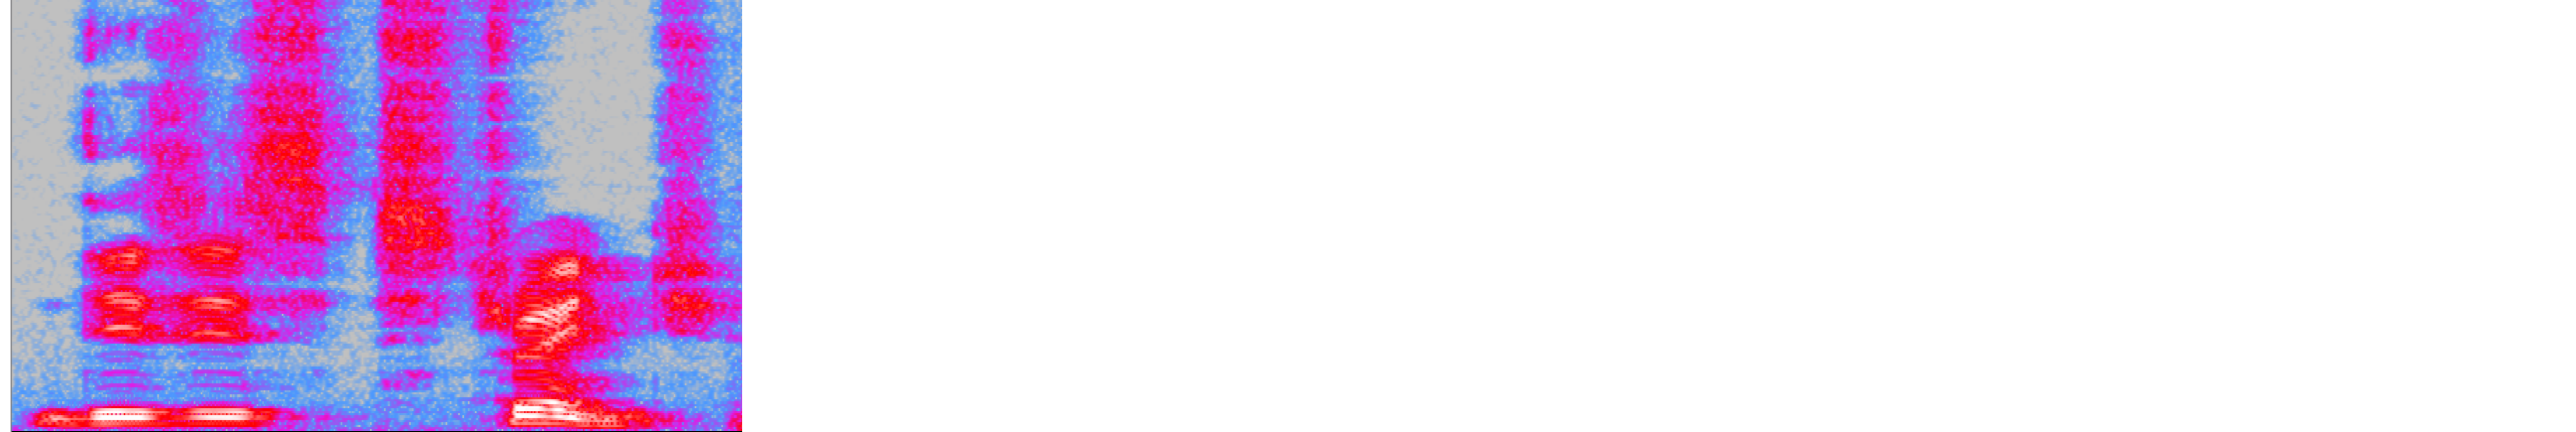
\includegraphics[width=0.8\textwidth]{images/spectrogram_cut.png}}%
\only<2>{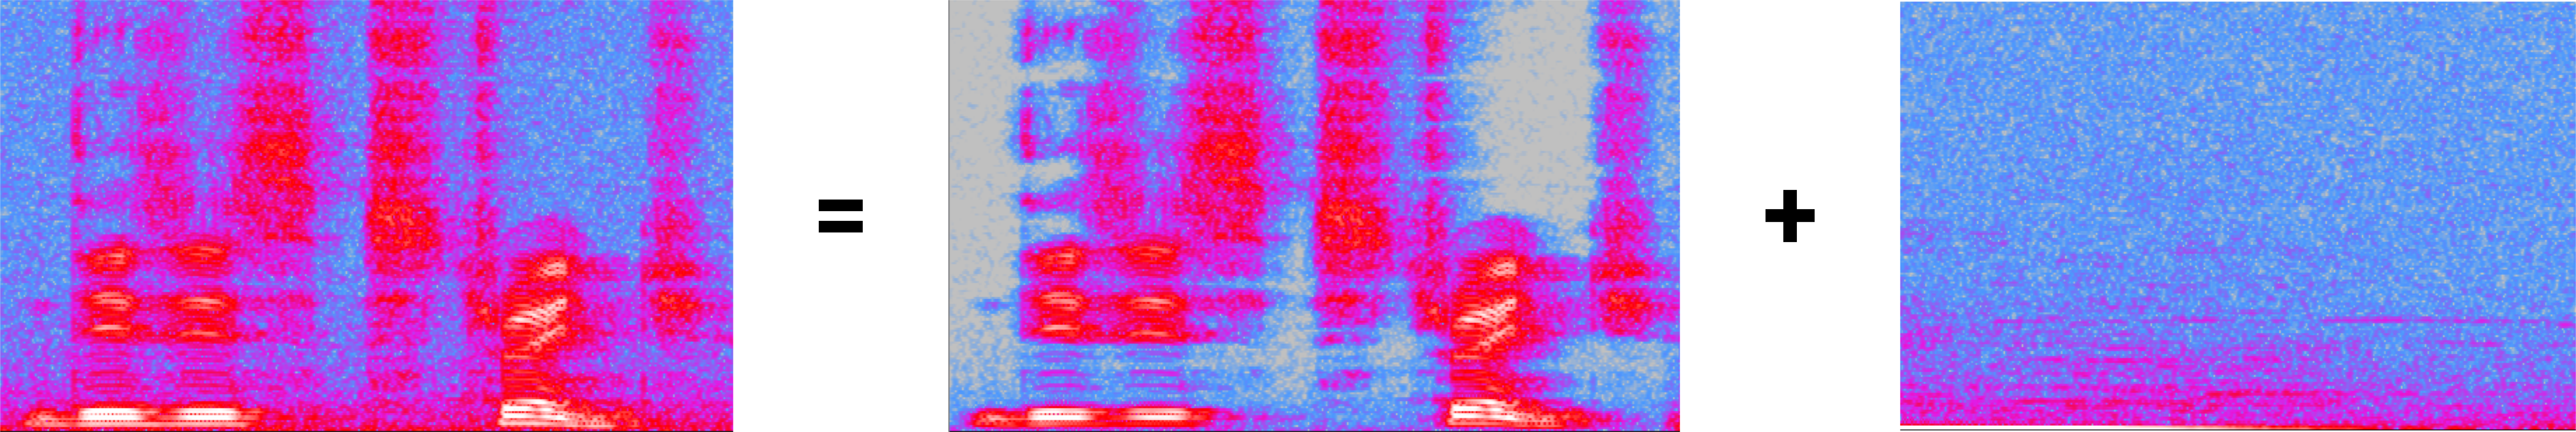
\includegraphics[width=0.8\textwidth]{images/spectrogram.png}}
\end{figure}
\vspace{-6mm}
\begin{equation*}
\only<1>{{\color{green}\underbrace{\mathbf{s}}_{\text{Clean speech}}} {\color{white}+\underbrace{\mathbf{b}}_{\text{Noise signal}}  = {\underbrace{\mathbf{x}}_{\text{Noisy mixture}}}}}
\only<2>{{\color{red}\underbrace{\mathbf{s}}_{\text{Clean speech}}} + {\color{gray}\underbrace{\mathbf{b}}_{\text{Noise signal}}}  ={\color{green}\underbrace{\mathbf{x}}_{\text{Noisy mixture}}}}
\end{equation*}


 \alert<1>{\textbf{Train}} -- Model $\alert<1>{\bs{\theta}}$ for \textcolor<1>{green}{clean data}: $\{{\only<1>{\color{green}}\bs{s}_{1:T}}\}$.
    \begin{center}
    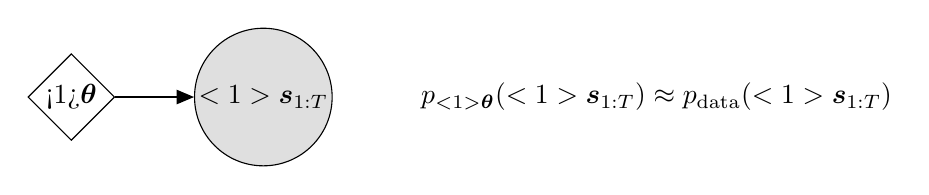
\begin{tikzpicture}
            \node[det] (theta) {\alert<1>{$\bs{\theta}$}};
            \node[obs,right=of theta] (s) {$\only<1>{\color{green}}\bs{s}_{1:T}$};
            \node[right=of s] (disc) {$p_{\alert<1>{\bs{\theta}}}({\only<1>{\color{green}}\bs{s}_{1:T}})\approx p_{\text{data}}({\only<1>{\color{green}}\bs{s}_{1:T}})$};
            \edge{theta} {s};
    \end{tikzpicture}\vspace{3mm}
    \includegraphics[width=0.5\textwidth]{images/NC-RVAE.png}\vspace{-3mm}
    \end{center}

 \end{column}\pause
 \begin{column}{0.5\textwidth}
  \textbf{Test} -- learn the \alert{noise parameters} from {\color{green} noisy samples $\mathbf{x}$} and estimate the {\color{red} clean speech $\hat{\bs{s}}_{1:T}$}:
    \begin{center}
    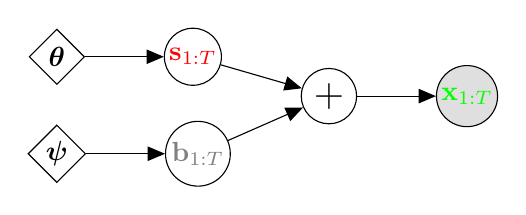
\begin{tikzpicture}
            \node[det] (theta) {$\bs{\theta}$};
            \node[latent,right=of theta] (s) {$\color{red}\mathbf{s}_{1:T}$};
            \node[det,below=of theta,yshift=5mm] (eta) {$\alert{\bs{\psi}}$};
            \node[latent,right=of eta] (b) {$\color{gray}\mathbf{b}_{1:T}$};
            \node[latent,right=of s,yshift=-5mm] (plus) {\Large$+$};
            \node[obs,right=of plus] (x) {$\color{green}\mathbf{x}_{1:T}$};
            \edge{theta} {s};
            \edge{eta} {b};
            \edge{s,b} {plus};
            \edge{plus} {x};
    \end{tikzpicture}\vspace{3mm}
      \includegraphics[width=0.5\textwidth]{images/NC-RVAE-test.png}\vspace{-3mm}
    \end{center}
 \end{column}
\end{columns}

% \textbf{Note}: at test time, $\bs{\theta}$ is frozen, and $\mathbf{s}$ becomes a latent variable.
\end{frame}

% %%%%%%%%%%%%%%%%%%%%%%%%%%%%%%%%%%%%%%%%%%%%%%%%%%%%%%%%%%%%%%%%%%%%%%%%%%%%
% \begin{frame}{Pre-training and Parameter Learning\footnote{Bie, X., \textit{et. al.}, (2022), IEEE TASLP.}}
%  \centering
%  \includegraphics[width=0.8\textwidth]{images/pre-training-dvae.png}\pause\vspace{2mm}
%  \hrule
%   \includegraphics[width=0.8\textwidth]{images/em-noise-dvae.png}
% \end{frame}

%%%%%%%%%%%%%%%%%%%%%%%%%%%%%%%%%%%%%%%%%%%%%%%%%%%%%%%%%%%%%%%%%%%%%%%%%%%%
\begin{frame}{Results on the Wall Street Journal (WSJ) and VoiceBank (VB)\footnote{Bie, X., \textit{et. al.}, (2022), IEEE TASLP.}}
% \includegraphics[width=0.5\textwidth]{images/speech-enhancement-same-dataset.png}\includegraphics[width=0.5\textwidth]{images/speech-enhancement-different-dataset.png}
% \textcolor{red}{Put colors!}
\centering
\scalebox{1.1}{
\setlength{\tabcolsep}{1.2mm}{\scriptsize%
\begin{tabular}{l cccc ccccc}
Method & Superv.& Test & Train & SI-SDR (dB) & Train & SI-SDR (dB) \\
\rowcolor{gray!40}
Noisy mixture & - &  & - & $-$2.6 & - & $-$2.6 \\
\rowcolor{green!40}
VAE-VEM~ (ICASSP'20) & None &  & & 5.0 \only<3->{& & 3.8} \\
% \rowcolor{green!40}Proposed DKF-VEM & UA & WSJ0-QUT & WSJ0 & 5.1 \only<3->{& VB & 3.5}\\
\rowcolor{green!40} RVAE-VEM (Proposed) & None & & & \textbf{5.8} \only<3->{&  & \textbf{4.3}} \\
% \rowcolor{green!40}Proposed SRNN-VEM & UA & WSJ0-QUT & WSJ0 & 5.2 \only<3->{& VB & \textbf{4.6}} \\
% \rowcolor{orange!40}MetricGAN-U (full)~ICASSP'22 & UD & WSJ0-QUT & WSJ0-QUT & N/A \only<3->{& VB-DMD & -2.3} \\
\rowcolor{orange!40}MetricGAN-U (ICASSP'22) & Partial & & &
N/A \only<3->{&  & -1.6} \\
% \hrule
\rowcolor{red!40}UMX*~2020 & Full &  & & \underline{5.7} \only<3->{&  & \underline{4.1}}\\
\rowcolor{red!40}MetricGAN+* (Interspeech'21) & Full & \multirow{-6}{*}{\rotatebox[origin=c]{90}{WSJ+QUT}} & \multirow{-5}{*}{\rotatebox[origin=c]{90}{Same}} &
3.6 \only<3->{& \multirow{-5}{*}{\rotatebox[origin=c]{90}{Different}} & 1.8} \\ \vspace{-2mm}\\
\rowcolor{gray!40}Noisy mixture & - \only<2->{& & - & 8.4 & - & 8.4} \\
\rowcolor{green!40}VAE-VEM (ICASSP'20) & None \only<2->{& & & 16.4 \only<4->{& & \underline{15.0}}} \\
% \rowcolor{green!40}Proposed DKF-VEM & UA \only<2->{& VB-DMD & VB & 16.9 \only<4->{& WSJ0 & 16.8}} \\
% Ours (RVAE-C) & \Checkmark & VB & VB-DMD &
% 16.4 & 3.22 & 2.46 & 3.15 & 0.81  \\
\rowcolor{green!40} RVAE-VEM (Proposed) & None \only<2->{& & & \underline{17.1} \only<4->{& & \textbf{17.3}}}  \\
% \rowcolor{green!40}Proposed SRNN-VEM & UA \only<2->{& VB-DMD & VB & 14.2 \only<4->{& WSJ0 & 16.8}} \\
\rowcolor{orange!40}NyTT~EUSIPCO'21 & Partial/Xtra \only<2->{& &  & \textbf{17.7} \only<4->{& & N/A}}\\
% \rowcolor{orange!40}NyTT~EUSIPCO'21 & UD \only<2->{& VB-DMD & VB-DMD & 12.1 \only<4->{& WSJ0-QUT & N/A}} \\
% \rowcolor{orange!40}MetricGAN-U (full)~ICASSP'22 & UD \only<2->{& VB-DMD  & VB-DMD & 6.5 \only<4->{& WSJ0-QUT & N/A}} \\
\rowcolor{orange!40}MetricGAN-U (half)~ICASSP'22 & Partial \only<2->{& & & 8.2 \only<4->{& & N/A}} \\
\rowcolor{red!40}UMX~2020  & Full \only<2->{& & &
14.0 \only<4->{& & 10.4}}  \\
\rowcolor{red!40}MetricGAN+ Interspeech'21 & Full \only<2->{& \multirow{-7}{*}{\rotatebox[origin=c]{90}{VB-DMD}}  & \multirow{-6}{*}{\rotatebox[origin=c]{90}{Same}} & 8.5 \only<4->{& \multirow{-6}{*}{\rotatebox[origin=c]{90}{Different}} & 3.9}} \\
\end{tabular}}}\vspace{2mm}

Results in dB: \textbf{best} and \underline{second best} per section.
\end{frame}

%%%%%%%%%%%%%%%%%%%%%%%%%%%%%%%%%%%%%%%%%%%%%%%%%%%%%%%%%%%%%%%%%%%%%%%%%%%%
{\setbeamercolor{background canvas}{bg=mDarkTeal}
\setbeamercolor{background canvas}{fg=white}
\begin{frame}%{Restricted to RNN?}
\begin{columns}
 \centering
 \begin{column}{0.7\textwidth}
  \color{white}\large\bf
   DVAEs are good (great!) at temporal modeling!\vspace{3mm}\\
   All implementations use RNN (or variants).\vspace{9mm}\\
   $\blacktriangleright$ What about transformers?
 \end{column}
\end{columns}\vspace{1cm}
\begin{columns}
 \begin{column}{3cm}
    \centering
    \includegraphics[width=.66\textwidth]{people/xiaoyu.png}\\
    \color{white}Xiaoyu Bie
 \end{column}
  \begin{column}{3cm}
    \centering
    \includegraphics[width=.66\textwidth]{people/wen.png}\\
    \color{white}Wen Guo
 \end{column}
  \begin{column}{3cm}
    \centering
    \includegraphics[width=.66\textwidth]{people/simon.png}\\
    \color{white}Simon Leglaive
 \end{column}
 \begin{column}{3cm}
    \centering
    \includegraphics[width=.66\textwidth]{people/francesc.png}\\
    \color{white}Francesc Moreno
 \end{column}
 \begin{column}{3cm}
    \centering
    \includegraphics[width=.66\textwidth]{people/laurent.png}\\
    \color{white}Laurent Girin
 \end{column}
\end{columns}\vspace{-2cm}
\end{frame}
}

%%%%%%%%%%%%%%%%%%%%%%%%%%%%%%%%%%%%%%%%%%%%%%%%%%%%%%%%%%%%%%%%%%%%%%%%%%%%
\begin{frame}{Introducing HIT-DVAE\footnote{Bie, X., \textit{et. al.}, (2023), Pre-print.}}
 Hierarchical Transformer DVAE -- two levels of latent variables: \textcolor{blue!50}{static $w$} and \textcolor{orange!70}{dynamic $z_{1:T}$}.
 \begin{figure}
  \includegraphics[width=\textwidth]{images/pipeline_hitdvae.png}\vspace{-3mm}
 \end{figure}
 \pause
 There is something \alert{odd} in the way Q, K, V are used...
\end{frame}

%%%%%%%%%%%%%%%%%%%%%%%%%%%%%%%%%%%%%%%%%%%%%%%%%%%%%%%%%%%%%%%%%%%%%%%%%%%%
\begin{frame}{HIT-DVAE: Modified transformer architecture}
   Task: human motion modeling/generation. Predicting $\bs{x}_{O+1}$ from $\bs{x}_{1:O}$ is very easy.\footnote{Guo., W., \textit{et. al.}, (2021), IEEE WACV.}\vspace{-6mm}
    \begin{figure}
     \centering
     \includegraphics[width=0.4\textwidth]{images/motion_generation}
    \end{figure}\vspace{-3mm}\pause%
   \begin{columns}
  \begin{column}{0.5\textwidth}
  \centering
    Standard query/residual connection:
     \includegraphics[width=0.7\textwidth]{images/transformer_arch_standard.png}
  \end{column}\pause%
  \begin{column}{0.5\textwidth}
  \centering
    HIT-DVAE query/residual connection:
     \includegraphics[width=0.7\textwidth]{images/transformer_arch_modified.png}
  \end{column}%
 \end{columns}
\end{frame}

%%%%%%%%%%%%%%%%%%%%%%%%%%%%%%%%%%%%%%%%%%%%%%%%%%%%%%%%%%%%%%%%%%%%%%%%%%%%
\begin{frame}{HIT-DVAE: Results}
\begin{figure}
 \centering
 \includegraphics[width=0.8\textwidth]{images/hitdvae_results}\vspace{-4mm}
\end{figure}
Good trade-off between diversity, quality and accuracy. Also useful for audio modeling.\footnote{Lin, X., \textit{et. al.}, (2023), IEEE ICASSP.}
\end{frame}

%%%%%%%%%%%%%%%%%%%%%%%%%%%%%%%%%%%%%%%%%%%%%%%%%%%%%%%%%%%%%%%%%%%%%%%%%%%%
{\setbeamercolor{background canvas}{bg=mDarkTeal}
\setbeamercolor{background canvas}{fg=white}
\begin{frame}%{Restricted to RNN?}
\begin{columns}
 \centering
 \begin{column}{0.7\textwidth}
  \color{white}\large\bf
   DVAEs can model mono-modal sequences.\vspace{9mm}\\
   $\blacktriangleright$ What about multiple modalities?
 \end{column}
\end{columns}\vspace{1cm}
\begin{columns}
 \begin{column}{3cm}
    \centering
    \includegraphics[width=.66\textwidth]{people/samir.png}\\
    \color{white}Samir Sadok
 \end{column}
  \begin{column}{3cm}
    \centering
    \includegraphics[width=.66\textwidth]{people/simon.png}\\
    \color{white}Simon Leglaive
 \end{column}
  \begin{column}{3cm}
    \centering
    \includegraphics[width=.66\textwidth]{people/renaud.png}\\
    \color{white}Renaud Séguier
 \end{column}
 \begin{column}{3cm}
    \centering
    \includegraphics[width=.66\textwidth]{people/laurent.png}\\
    \color{white}Laurent Girin
 \end{column}
\end{columns}\vspace{-2cm}
\end{frame}
}


%%%%%%%%%%%%%%%%%%%%%%%%%%%%%%%%%%%%%%%%%%%%%%%%%%%%%%%%%%%%%%%%%%%%%%%%%%%%
\begin{frame}{In other words:}
 \begin{figure}
  \centering
  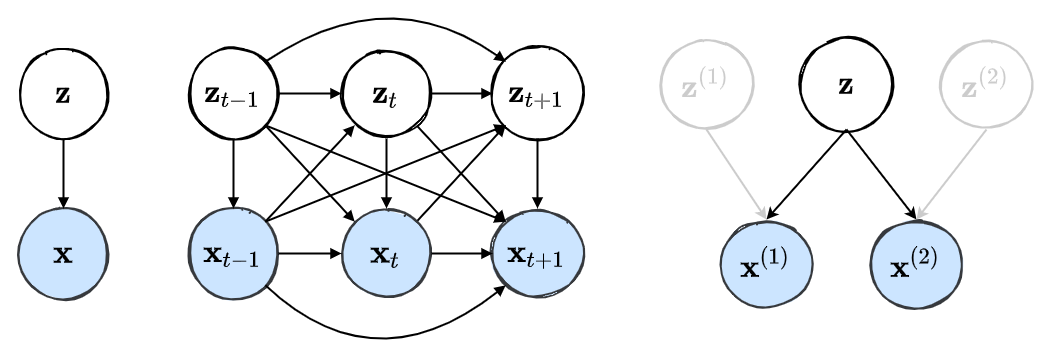
\includegraphics[width=0.7\textwidth]{images/BN_VAE_DVAE_MVAE-mod.png}
 \end{figure}
 VAEs (left) can be multi-modal\footnote{Sutter, T. M., \textit{et. al.}, (2021), ICLR.} (right). Can DVAEs (middle) be multi-modal too?
\end{frame}

%%%%%%%%%%%%%%%%%%%%%%%%%%%%%%%%%%%%%%%%%%%%%%%%%%%%%%%%%%%%%%%%%%%%%%%%%%%%
\begin{frame}{Task: emotional audio-visual speech modeling.\footnote{Wang, K., \textit{et. al.}, (2020), ECCV.}}
\begin{columns}
\centering
\begin{column}{0.6\textwidth}
  \includegraphics[width=\textwidth]{images/mead.png}
 \end{column}
 \hfill
  \begin{column}{0.28\textwidth}
    \small
    What should we model?
    \begin{itemize}
     \item Static AV\\ (ID, emotion)
     \item Dynamic AV\\ (lip-audio corr.)
     \item Dynamic A\\ (other audio features)
     \item Dynamic V\\ (eye AUs).
    \end{itemize}
  \end{column}
\end{columns}

\end{frame}

%%%%%%%%%%%%%%%%%%%%%%%%%%%%%%%%%%%%%%%%%%%%%%%%%%%%%%%%%%%%%%%%%%%%%%%%%%%%
\begin{frame}{Introducing MDVAEs\footnote{Sadok, S., \textit{et. al.}, (2024), Neural Networks.}}
%  \begin{figure}
%   \centering
%   \includegraphics[width=1\textwidth]{images/diagram_MDVAE}
%   \end{figure}
  \begin{columns}
\centering
\begin{column}{0.7\textwidth}
    \includegraphics[width=1\textwidth]{images/diagram_MDVAE}\end{column}
    \hfill
  \begin{column}{0.28\textwidth}
    \small
    What should we model?
    \begin{itemize}
     \item Static AV -- $\bs{w}$\\ (ID, emotion)
     \item Dynamic AV -- $\bs{z}^{av}$\\ (lip-audio corr.)
     \item Dynamic A -- $\bs{z}^{a}$\\ (other audio features)
     \item Dynamic V -- $\bs{z}^{v}$\\ (eye AUs).
    \end{itemize}
  \end{column}
\end{columns}

\end{frame}

%%%%%%%%%%%%%%%%%%%%%%%%%%%%%%%%%%%%%%%%%%%%%%%%%%%%%%%%%%%%%%%%%%%%%%%%%%%%
\begin{frame}{The VQ-MDVAE Architecture}
 \begin{figure}
  \centering
  \includegraphics[width=1\textwidth]{images/overview-VQMDVAE}
  \end{figure}
 (i) Quantize auditory and visual features. (ii) Use MDVAE to model the quantized features.
\end{frame}

%%%%%%%%%%%%%%%%%%%%%%%%%%%%%%%%%%%%%%%%%%%%%%%%%%%%%%%%%%%%%%%%%%%%%%%%%%%%
\begin{frame}{MDVAE: Some fun things}
Let's see a couple of videos on:\vspace{5mm}
\begin{itemize}
  \item latent variable transfer,\vspace{5mm}
  \item latent variable interpolation.
 \end{itemize}
\end{frame}
%
% %%%%%%%%%%%%%%%%%%%%%%%%%%%%%%%%%%%%%%%%%%%%%%%%%%%%%%%%%%%%%%%%%%%%%%%%%%%%
% \begin{frame}{MDVAE: Latent variable transfer}
% \begin{columns}
% \begin{column}{0.4\textwidth}
%  \centering
%  $\bs{z}^{av}$\vspace{2mm}\\
% \fbox{\movie[height = \textwidth, width = \textwidth, poster, showcontrols]{}{videos/mdvae_z_av.mp4}}\\
% Transfered lip and jaw movements.
%  \end{column}\pause
% \begin{column}{0.4\textwidth}
%  \centering
%  $\bs{z}^{v}$\vspace{2mm}\\
%  \fbox{\movie[height = \textwidth, width = \textwidth, poster, showcontrols]{}{videos/mdvae_z_visual.mp4}}\\
% Transfered head and eyelid.
% \end{column}
% \end{columns}
%
% \end{frame}
%
% %%%%%%%%%%%%%%%%%%%%%%%%%%%%%%%%%%%%%%%%%%%%%%%%%%%%%%%%%%%%%%%%%%%%%%%%%%%%
% \begin{frame}{MDVAE: Latent variable interpolation}
% \begin{columns}
% \begin{column}{0.4\textwidth}
%  \centering
% \fbox{\movie[height = \textwidth, width = \textwidth, poster, showcontrols]{}{videos/mdvae_identity_interpolation.mp4}}\\
% Same emotion, different ID.
%  \end{column}\pause
% \begin{column}{0.4\textwidth}
%  \centering
%  \fbox{\movie[height = \textwidth, width = \textwidth, poster, showcontrols]{}{videos/mdvae_emotions_interpolation.mp4}}\\
% Same ID, different emotion.
% \end{column}
% \end{columns}
% \end{frame}

%%%%%%%%%%%%%%%%%%%%%%%%%%%%%%%%%%%%%%%%%%%%%%%%%%%%%%%%%%%%%%%%%%%%%%%%%%%%
{\setbeamercolor{background canvas}{bg=mDarkTeal}
\setbeamercolor{background canvas}{fg=white}
\begin{frame}%{Restricted to RNN?}
\begin{columns}
 \centering
 \begin{column}{0.7\textwidth}
  \color{white}\large\bf
   Earlier, we combined (static) VAEs with \underline{mixing} latents.\vspace{9mm}\\
   $\blacktriangleright$ Is it possible/useful with DVAEs?
 \end{column}
\end{columns}\vspace{1cm}
\begin{columns}
 \begin{column}{3cm}
    \centering
    \includegraphics[width=.66\textwidth]{people/xiaoyulin.png}\\
    \color{white}Xiaoyu Lin
 \end{column}
 \begin{column}{3cm}
    \centering
    \includegraphics[width=.66\textwidth]{people/laurent.png}\\
    \color{white}Laurent Girin
 \end{column}
\end{columns}\vspace{-2cm}
\end{frame}
}

%%%%%%%%%%%%%%%%%%%%%%%%%%%%%%%%%%%%%%%%%%%%%%%%%%%%%%%%%%%%%%%%%%%%%%%%%%%%
\begin{frame}{Motivating application: unsupervised multiple object tracking}
\begin{columns}
 \begin{column}{3cm}
  \centering
  \includegraphics[width=\textwidth]{images/tracklets_mixdvae}
  Tracklets @ $t-1$
 \end{column}
 \begin{column}{3cm}
  \centering
  \includegraphics[width=.66\textwidth]{images/detections_mixdvae}
  Detections @ $t$
 \end{column}
 \begin{column}{3cm}
  \centering
  \includegraphics[width=.66\textwidth]{images/assignment_mixdvae}
  Desired result
 \end{column}
\end{columns}\vspace{1cm}
\textbf{Question}: Can we model the non-linear dynamics with a DVAE, and have an assignment mechanism within the same ML formulation?
\end{frame}

%%%%%%%%%%%%%%%%%%%%%%%%%%%%%%%%%%%%%%%%%%%%%%%%%%%%%%%%%%%%%%%%%%%%%%%%%%%%
\begin{frame}{Introducing MixDVAE\footnote{Lin, X., \textit{et. al.}, (2023), Under review.}}
 \begin{figure}
  \centering
  \only<1>{\includegraphics[width=\textwidth]{images/MixDVAE_algo_pretrain.pdf}}%
  \only<2>{\includegraphics[width=\textwidth]{images/MixDVAE_algo_input.pdf}}%
  \only<3>{\includegraphics[width=\textwidth]{images/MixDVAE_algo_prediction.pdf}}%
  \only<4>{\includegraphics[width=\textwidth]{images/MixDVAE_algo_algorithm.pdf}}%
  \only<5>{\includegraphics[width=\textwidth]{images/MixDVAE_algo_inference.pdf}}%
  \only<6>{\includegraphics[width=\textwidth]{images/MixDVAE_algo_learning.pdf}}%
 \end{figure}
\end{frame}

%%%%%%%%%%%%%%%%%%%%%%%%%%%%%%%%%%%%%%%%%%%%%%%%%%%%%%%%%%%%%%%%%%%%%%%%%%%%
\begin{frame}{Quick discussion \& results}
\begin{columns}
 \begin{column}{0.5\textwidth}
  \centering GMM update ($K$ observations):
  \[\bs{\mu}_n = \sum_{k} \underbrace{\eta_{kn}}_{\text{assign.}} \bs{o}_k\]
 \end{column}\pause
 \begin{column}{0.5\textwidth}
  \centering Kalman update (sequence of $T$ obs):
  \[\bs{s}_t = \underbrace{\bs{P}_t\bs{o}_t}_{\text{update}} + \underbrace{\bs{T}_t\bs{s}_{t-1}}_{\text{prediction}}\]
 \end{column}
\end{columns}\pause
%  Standard GMM (left) and Kalman filter (right) updates:
%  \[
%   n\text{-th center:}\quad \qquad \qquad \text{position @$t$:}\quad\bs{s}_t = \underbrace{\bs{P}_t\bs{o}_t}_{\text{update}} + \underbrace{\bs{T}_t\bs{s}_{t-1}}_{\text{prediction}}
%  \]\pause
 \[\text{MixDVAE update is a combination:}\quad \bs{s}_{tn} = \underbrace{\bs{P}_t\sum_{k} \eta_{kn}\bs{o}_{tk}}_{\text{assig. \& update}} + \underbrace{\bs{T}_t(\bs{s}_{1:t-1})}_{\text{non-lin. prediction}} \vspace{-3mm} \]\pause
\begin{itemize}
 \item Results in unsupervised MOT and in semi-blind source separation.
 \item Work in progress: fine-tuning, complexity, learning from noise, ...
\end{itemize}

\end{frame}

%%%%%%%%%%%%%%%%%%%%%%%%%%%%%%%%%%%%%%%%%%%%%%%%%%%%%%%%%%%%%%%%%%%%%%%%%%%%
{\setbeamercolor{background canvas}{bg=mDarkTeal}
\setbeamercolor{background canvas}{fg=white}
\begin{frame}{VAE/DVAE Summary}
\textcolor{white}{ \begin{tabular}{cccc}
 \toprule
  & \textbf{Mono-modal} & \textbf{Multi-modal} & \textbf{Mixtures} \\\midrule
 \textbf{Static} & \makecell{VAE [Kingma'14]\\ VQ-VAE [van den Oord'17]} & \only<2->{\makecell{CVAE [Sadeghi'20]\\ MVAE [Sutter'21]}} & \only<3->{\makecell{VAE-MM [Sadeghi'20]\\ MIN-VAE [Sadeghi'21]}}\\\midrule
 \textbf{Dynamic} & \only<4->{\makecell{DVAE [Girin'21]\\ Sw-VAE [Sadeghi'21]}} & \only<5->{VQ-MDVAE [Sadok'23]} & \only<6->{MixDVAE [Lin'23]}\\\bottomrule
 \end{tabular}}
\end{frame}}

%%%%%%%%%%%%%%%%%%%%%%%%%%%%%%%%%%%%%%%%%%%%%%%%%%%%%%%%%%%%%%%%%%%%%%%%%%%%
\begin{frame}{Limited to VAE? NO!}
 We started investigated unsupervised AVSE with diffusion models:
 \includegraphics[width=\textwidth]{images/AVDiffuse.png}
 Still need an EM algorithm at test time...
\end{frame}

\begin{frame}{What else is there to be done?}
 Plenty!!!
 \begin{itemize}
  \item Systematic AV for diffusion works.
  \item Can we design mixtures of diffusion models?
  \item What about latent diffusion?
  \item Can we have mixtures combined with latent diffusion?
  \item What about temporal diffusion models? And their mixtures?
  \item And beyond diffusion? e.g. flow matching?
 \end{itemize}
\end{frame}

%%%%%%%%%%%%%%%%%%%%%%%%%%%%%%%%%%%%%%%%%%%%%%%%%%%%%%%%%%%%%%%%%%%%%%%%%%%%
{\setbeamercolor{background canvas}{bg=mDarkTeal}
\setbeamercolor{background canvas}{fg=white}
\begin{frame}
 \color{white}\Large \bf Summary \& conclusions
\end{frame}}

\begin{frame}{Take-home messages}
 \begin{itemize}
  \item Latent variable modlings has endless possiblities.
  \item Auto-grad cannot save you.
  \item Analytic results can bring interpretability.
  \item Many possibilities are yet to be explored.\\
  \item Uncommon skills/knowledge (e.g. VI) can make your profile unique.
 \end{itemize}

\end{frame}

%%%%%%%%%%%%%%%%%%%%%%%%%%%%%%%%%%%%%%%%%%%%%%%%%%%%%%%%%%%%%%%%%%%%%%%%%%%%
\begin{frame}{Thanks...}
\centering
 \begin{columns}
  \begin{column}{0.5\textwidth}
   \includegraphics[width=\textwidth]{images/team}
  \end{column}
  \begin{column}{0.4\textwidth}
   for bearing with me!\vspace{3mm}\\
   to my colleagues \& collaborators!\vspace{3mm}\\
   for your challenging questions\\ \& interesting discussion.\vspace{8mm}\\
   We are also interested in meta- learning, reinforcement learning, domain adaptation, etc.\vspace{3mm}\\
   I am around until Thursday!
  \end{column}
 \end{columns}

\end{frame}


\end{document}
